\documentclass[12pt,twoside]{book}

%%%%%%%%%%%%%%%%%%%%%%%%%%%
%%%%%%%%%%%%%%%%%%%%%%%%%%%

\usepackage[toc,page]{appendix}
\usepackage[hyperfootnotes=false,colorlinks=false,backref=false]{hyperref}
\usepackage{bookmark}
\usepackage{hyphenat}
\usepackage[perpage,symbol*]{footmisc}	% Footnote counter reset per page

\usepackage{amsmath}			% See amsldoc.pdf for more information.
\usepackage{amsthm}			% See amsthdoc.pdf for more information.

\usepackage{geometry}                	% See geometry.pdf to learn the layout options.
\geometry{a4paper}                   		% ... or a4paper or a5paper or ... 
\geometry{inner = 3.4cm, outer = 3.4cm}
\geometry{top = 4cm, bottom = 4.6cm}
\setlength{\parskip}{0cm}

\usepackage[dutch,english]{babel}	% English default
\usepackage{pifont}
\usepackage{graphicx}
\usepackage{amssymb}
\usepackage{epstopdf}
\usepackage[usenames,dvipsnames]{color}
\DeclareGraphicsRule{.tif}{png}{.png}{`convert #1 `dirname #1`/`basename #1 .tif`.png}
\usepackage{mdwlist}			% Lists with paragraph spacing between items, use itemize*

\usepackage{xcolor,textpos}
\usepackage{verbatim}

\linespread{1.1}

%\widowpenalty=300
%\clubpenalty=300




%Declaration for the amsthm package
%-------------------------------------------------
\newtheorem{definition}{Definition}[chapter]
\newtheorem{theorem}{Theorem}[chapter]

\newcommand\real{\operatorname{Re}}
\newcommand\imag{\operatorname{Im}}


%Style chapters
%-------------------
\usepackage[PetersLenny]{fncychap}

%Style headers
%-------------------
\usepackage{fancyhdr}
\pagestyle{fancy}

%%%%%%%%%%%%%%%%%%%%%%%%%%%
%%%%%%%%%%%%%%%%%%%%%%%%%%%
\begin{document}


% ----------------------- Cover --------------------------------------
% Please fill in:
% - The department and section
% - The title and subtitle (if applicable)
% - Your name
% - Your (co)supervisor, mentor (if applicable)
% - Your master 
% - The academic year
% --------------------------------------------------------------------
\begin{titlepage}
\thispagestyle{empty}

\definecolor{gray}{rgb}{0.600,0.600,0.600}
\setlength{\TPHorizModule}{1mm}
\setlength{\TPVertModule}{1mm}

\topmargin -10mm
\textwidth 160truemm
%\textheight 240truemm
\oddsidemargin 0mm
%\evensidemargin 0mm

\begin{textblock}{160}(0,-32.5)
\vspace{-\parskip}
\begin{center}

\includegraphics[width=10.3mm]{sedes}
\end{center}
\end{textblock}
%
\begin{textblock}{140}(38.4,-7)
\colorbox{gray}{\hspace{15mm}\ \parbox[c][21.4truemm]{122mm}{
{\sffamily{\bf \fontsize{14}{16} \selectfont \sffamily \textcolor{white} {FACULTY OF SCIENCE}}\\
{\fontsize{12}{14} \selectfont \textcolor{white} {Department of Physics}}\\
{\fontsize{12}{14} \selectfont \textcolor{white} {Institute for Theoretical Physics}}
}}}
\end{textblock}
%
\begin{textblock}{70}(-31.6,-6.9)
\textblockcolour{}
\includegraphics*[width=70truemm]{kuleuven}
\end{textblock}
%
\begin{textblock}{160}(0,80)
\textblockcolour{}
\vspace{-\parskip}
\begin{center}
\fontsize{16}{18} \selectfont \sffamily\textbf{
The black hole entropy function in the presence of\\
a gauge Chern-Simons term in five dimensions}\vspace{3mm}

%\fontsize{14}{16} \textbf{Subtitle} \textit{(optional)}
\end{center}
\end{textblock}
%
\begin{textblock}{160}(0,120)
\textblockcolour{}
\vspace{-\parskip}
\begin{center}
\fontsize{12}{14}\selectfont \sffamily{by}
\end{center}
\end{textblock}
%
\begin{textblock}{160}(0,150)
\textblockcolour{}
\vspace{-\parskip}
\begin{center}
\fontsize{12}{14}\selectfont\sffamily{
Hendrik Jennen}
\end{center}
\end{textblock}
%
\begin{textblock}{160}(0,215)
\textblockcolour{}
\vspace{-\parskip}
\begin{tabular}{p{10cm}l}
 \sffamily{Supervisor: Dr.\ Jan Perz}  			& \sffamily{Dissertation presented in} \\
									& \sffamily{fulfillment of the requirements}\\
									& \sffamily{for the degree of Master in} \\
									& \sffamily{Theoretical Physics}
\end{tabular}
\end{textblock}
%
\begin{textblock}{160}(0,240)
\textblockcolour{}
\vspace{-\parskip}
\begin{center} \sffamily{Academic year 2009-2010} \end{center}
\end{textblock}
\vfill
\end{titlepage}
%----------------------------------------------

%%%%%%%%%%%%%%%%%%%%%%%%%%%
%%%%%%%%%%%%%%%%%%%%%%%%%%%
\newpage
\thispagestyle{empty}

%%%%%%%%%%%%%%%%%%%%%%%%%%%
%%%%%%%%%%%%%%%%%%%%%%%%%%%
\begin{titlepage}
\thispagestyle{empty}

\definecolor{gray}{rgb}{0.600,0.600,0.600}
\setlength{\TPHorizModule}{1mm}
\setlength{\TPVertModule}{1mm}

\topmargin -10mm
\textwidth 160truemm
%\textheight 240truemm
\oddsidemargin 0mm
%\evensidemargin 0mm

\begin{textblock}{160}(0,15)
\vspace{-\parskip}
\begin{center}

\includegraphics[width=17mm]{sedes}
\end{center}
\end{textblock}
%
%
\begin{textblock}{160}(0,80)
\textblockcolour{}
\vspace{-\parskip}
\begin{center}
\fontsize{16}{18} \selectfont \sffamily\textbf{
The black hole entropy function in the presence of\\
a gauge Chern-Simons term in five dimensions}\vspace{3mm}

%\fontsize{14}{16} \textbf{Subtitle} \textit{(optional)}
\end{center}
\end{textblock}
%
\begin{textblock}{160}(0,120)
\textblockcolour{}
\vspace{-\parskip}
\begin{center}
\fontsize{12}{14}\selectfont \sffamily{by}
\end{center}
\end{textblock}
%
\begin{textblock}{160}(0,150)
\textblockcolour{}
\vspace{-\parskip}
\begin{center}
\fontsize{12}{14}\selectfont\sffamily{
Hendrik Jennen}
\end{center}
\end{textblock}
%
\begin{textblock}{160}(0,215)
\textblockcolour{}
\vspace{-\parskip}
\begin{tabular}{p{10cm}l}
 \sffamily{Supervisor: Dr. Jan Perz}  			& \sffamily{Dissertation presented in} \\
									& \sffamily{fulfillment of the requirements}\\
									& \sffamily{for the degree of Master in} \\
									& \sffamily{Theoretical Physics}
\end{tabular}
\end{textblock}
%
\begin{textblock}{160}(0,240)
\textblockcolour{}
\vspace{-\parskip}
\begin{center} \sffamily{Academic year 2009-2010} \end{center}
\end{textblock}
\vfill
\end{titlepage}
%%%%%%%%%%%%%%%%%%%%%%%%%%%
%%%%%%%%%%%%%%%%%%%%%%%%%%%
\newpage
\thispagestyle{empty}




%%%%%%%%%%%%%%%%%%%%%%%%%%%
%%%%%%%%%%%%%%%%%%%%%%%%%%%
\frontmatter



%----------------------------------------------
%TABLE OF CONTENTS
%----------------------------------------------

%Head style table of contents
%---------------------------------
\renewcommand{\chaptermark}[1]{%
\markboth{\chaptername%
\ \thechapter.%
\ #1}{}}

\renewcommand{\sectionmark}[1]{%
\markright{
\thesection%
\ #1}{}}

\fancyhead{} % clear all header fields
\fancyhead[RO,LE]{\thepage}
\fancyhead[RE]{\nouppercase{\leftmark}}
\fancyhead[LO]{\nouppercase{\rightmark}}
\fancyfoot{} % clear all footer fields
\renewcommand{\headrulewidth}{0.4pt}

%---------------------------------

\tableofcontents
%----------------------------------------------
\selectlanguage{english}


%----------------------------------------------
%ACKNOWLEDGEMENTS
%----------------------------------------------
\newpage
\thispagestyle{empty}
\mbox{}
\vfill
\noindent
\begin{LARGE}\textbf{Acknowledgements}\end{LARGE}\\

\noindent
In the first place, I would like to thank Dr.\ Jan Perz for his stimulating guidance and useful advice in the course of our research and for his suggested corrections regarding earlier versions of this text. I also would like to express my appreciation towards Johannes Oberreuter for sharing his interesting thoughts and to the readers Prof.\ N.\ Severijns and Prof.\ A.\ Van Proeyen. To those closest to me, I am deeply grateful for really a lot of reasons.

\newpage
\thispagestyle{empty}
%%%%%%%%%%%%%%%%%%%%%%%%%%%
\mainmatter


%Head style main document
%------------------------------------
\renewcommand{\chaptermark}[1]{%
\markboth{\chaptername%
\ \thechapter.%
\ #1}{}}

\renewcommand{\sectionmark}[1]{%
\markright{
\thesection%
\ #1}{}}

\fancyhead{} % clear all header fields
\fancyhead[RO,LE]{\thepage}
\fancyhead[RE]{\leftmark}
\fancyhead[LO]{\rightmark}
\fancyfoot{} % clear all footer fields
\renewcommand{\headrulewidth}{0.4pt}



%%%%%%%%%%%%%%%%%%%%%%%%%%%
\begin{comment}
\addtolength{\headheight}{\baselineskip}

\renewcommand{\chaptermark}[1]{%
\markboth{\chaptername%
\ \thechapter.%
\ #1}{}}


\renewcommand{\sectionmark}[1]{%
\markright{
\thesection%
\ #1}{}}

\lhead{\slshape \leftmark \\%
\rightmark}

\rhead{\thepage}

\fancyfoot{}
\end{comment}
%%%%%%%%%%%%%%%%%%%%%%%%%%%

%----------------------------------------------
%----------------------------------------------
%-----------------
%CHAPTER
%-----------------
%----------------------------------------------
\chapter{Introduction and motivation}
\label{ch:intro&motiv}

One of the principles at heart of fundamental science is the so called scheme of unification. In this scheme, one tries to describe apparently different phenomena observed in nature through one underlying principle, written down in the language of mathematics. Already in the second half of the 17th century Newtonian mechanics and gravitation described the motion of planets and the falling of an apple through the same set of laws. About two centuries later, at the end of the 19th century, the phenomena related to electricity, magnetism and light were unified, as synthesized in Maxwell's equations of electromagnetism. This unification implied the existence of electromagnetic waves and that light was in fact a special kind of these waves, which travelled all at a definite fixed speed. Unifying Maxwell's equations, and especially the consequence of a constant speed of light, with the principle of relativity\footnote{This principle states that the laws of physics are the same to every inertial observer.} one is led to special relativity. Einstein's general theory of relativity then incorporates gravity as a curving of space-time.

One of the basic consequences of general relativity is the existence of black holes. These very dense concentrations of mass curve space-time so strongly that anything that comes too close, cannot go back.\footnote{These points of no return constitute the \emph{horizon} of the black hole.} This is also true for light, hence the name \emph{black} holes. Although they were regarded as a mathematical curiosity at their theoretical discovery, they are by now widely believed to be a good description of objects residing in our universe. This existence of black holes in nature is a good reason to investigate them. However, there are other aspects regarding black holes which make them interesting to do research at. A reason can be found in the scheme of unification. Classically black holes do not seem to exhibit thermodynamical behavior. Because nothing can escape from them, they cannot radiate and thus have a zero absolute temperature. However, when the quantization of matter is taken into account in the vicinity of a black hole, Hawking showed that it does have the thermodynamical spectrum of a black body. 
In this semi-classical approximation, entropy is found to be proportional to the area of the black hole event horizon. From general relativity it follows that the latter increases in any physical process and thus may be correctly interpreted as a macroscopic entropy. The exact numerical relation between the entropy of a black hole and its event horizon area is given by the Bekenstein-Hawking formula. Having a macroscopic entropy at hand, one then may wonder how this entropy may be accounted for from a statistical point of view, i.e.\ how can the microscopic entropy be calculated?

In the scheme of unification, the theories of quantum mechanics and general relativity turn out to be rather difficult to reconcile.
On one hand, far away from space-time curving black holes quantum field theory proves to be in excellent agreement with experiment at the smallest length scales presently observable in nature.
On the other hand, general relativity has emerged as a successful model in describing the large scale behavior of gravitation and cosmology.
As we have seen, black holes---fundamental in general relativity---show thermodynamic behavior only when quantum mechanics is taken into account. This suggests that black holes are of great importance in the quest for a consistent theory of quantum gravity. Indeed, from the quantum mechanical nature of black hole thermodynamics, it is suggested that a statistical interpretation of the Bekenstein-Hawking entropy should be done in a framework of quantum gravity. In such a microscopic interpretation, the entropy is calculated through a counting over microstates as described in the unified theory.
Once the microscopic entropy for a given black hole configuration is found, the result can be compared with the macroscopic Bekenstein-Hawking entropy. In this view, black holes are very interesting as they may teach us a great deal about a unified theory of quantum mechanics and gravity.

Superstring theory is a candidate for a quantum theory of gravity and it reduces to  supergravity in the low-energy limit. The bosonic sectors of four- and five-dimensional supergravity theories describe gravity coupled to a set of scalar and vector fields.
When considering black hole solutions in theories where there are a number of scalar fields, their macroscopic entropy will generically depend on the values of the scalar fields at the horizon. 
The possibility then exists that these scalar fields at the horizon depend on asymptotic boundary conditions. This would make it impossible to give the macroscopic Bekenstein-Hawking entropy a statistical interpretation, since the latter should depend only on local---residing in the black hole---information of microscopic states corresponding to the macroscopic description of the black hole. However, it turns out that for a specific subclass of black hole solutions there exists a mechanism which drives the scalar fields at the horizon to definite values, depending only on the charges characterizing the black hole. This mechanism goes by the name of the \emph{attractor mechanism}. It was first discovered for supersymmetric black holes and later found to be at work also for extremal black hole solutions. One way of understanding the attractor mechanism for static and spherically symmetric extremal black holes is through the effective black hole potential, which attracts the scalars to their fixed values at the horizon. This was done for black hole solutions where higher curvature corrections could be neglected.

Another way of deriving the attractor mechanism for extremal black holes is through the entropy function formalism. In this formalism the entropy function is defined as the Legendre transform with respect to the electric fields of the Lagrangian integrated over the black hole horizon. This function has two practical properties. The first is that extremization of the entropy function with respect to the near horizon fields is equivalent to solving the corresponding equations of motion for the near horizon values. Secondly, evaluating the entropy function for the on-shell near horizon fields gives the entropy of the black hole. Since this entropy is given only by near horizon information of the different fields appearing in the theory, this allows for a microscopic interpretation of it. Moreover, the derivation of these properties is based on Wald's formula, which gives one the macroscopic entropy of a black hole in the presence of higher curvature corrections and reduces to the Bekenstein-Hawking formula when these corrections are not present.
As such, the entropy function formalism naturally lends itself to the description of the attractor mechanism for spherically symmetric extremal black holes in theories of higher derivative gravity.

Unfortunately this formalism is only valid under some specific assumptions, and thus has its limitations. One of them is that the vector fields should not appear explicitly in the action describing the theory, i.e.\ the vector fields should appear only through their associated field strengths. This is not the case for five-dimensional supergravity theories where the action contains Chern-Simons terms. The question one can pose and which was a motivation for this thesis is then: how to define an entropy function for theories in five dimensions containing Chern-Simons terms? So far several attempts have been made to extend the formalism to these theories. One of them makes use of dimensional reduction by placing a five-dimensional black hole in a Taub-NUT geometry. Since this geometry has one compact direction---a circle---one can interpolate naturally between a five- and four-dimensional description of the black hole, by varying the modulus of the circle. In this way five-dimensional black holes are connected to four-dimensional ones and for the latter the entropy function is well-defined. Apart from this approach it was proposed that a direct five-dimensional procedure is possible, i.e.\ one can consistently define a formalism in the presence of Chern-Simons terms. This approach makes use of the observation that there are different possible choices of charge associated with the gauge fields. This charge ambiguity also pops up in defining an entropy function and it seems that the correct quantity to use is the Page charge. In this thesis we will review the two mentioned proposals for the specific case of five-dimensional static spherically symmetric extremal black holes, and compare the results. In doing so, the two approaches seem not to be equivalent and we try to reconcile the apparent differences between them.
Furthermore, we argue why Page charge is the natural quantity to use in a five-dimensional formalism.\newline

\noindent
To conclude this introductory chapter let us give a brief outline of the thesis.
\begin{itemize}
\item[$\diamond$]
In chapter \ref{ch:mathBack} we present some mathematical background, which will be of use for the remainder of the text. We review the concepts of manifolds (real, almost complex, complex and K\"ahler), fiber bundles and differential forms. These are some of the basic mathematical objects with which the physics of gravity coupled to a set of bosonic fields is described.

\item[$\diamond$]
Chapter \ref{ch:physBack} tries to give a survey of some physical concepts connected to black holes and their entropy. First we review Einstein-Maxwell theory and the Reissner-Nordstr\"om black hole solutions. These solutions do not have scalar fields, but they allow us to introduce the concept of extremality in the simplest case possible.
We also review the subject of black hole thermodynamics where the macroscopic Bekenstein-Hawking entropy is introduced. Thereafter the structure of the bosonic side of four-dimensional $N=2$ supergravity is presented and BPS black hole solutions to this theory are considered, since these are extremal. We also explain the attractor mechanism at play for these BPS solutions and extend the mechanism to non-supersymmetric extremal black holes, by use of the black hole potential. Then the bosonic sector of five-dimensional $N=2$ supergravity is recalled and we will see that they have Chern-Simons terms appearing in the action. To conclude we review the ideas behind Kaluza-Klein theory as this will establish a connection between five- and four-dimensional black hole solutions in chapter \ref{ch:entrFunc&CS}.

\item[$\diamond$]
The entropy function formalism is introduced in chapter \ref{ch:entrFunc}, which gives us another way of understanding the attractor mechanism for extremal black hole solutions. Also the limitations of the formalism are discussed, as they become relevant in five-dimensional theories with Chern-Simons terms.

\item[$\diamond$]
Chapter \ref{ch:entrFunc&CS} reviews and compares two proposals for defining an entropy function for a five-dimensional theory of gravity, vector fields and scalars in the presence of Chern-Simons terms. We also explain the ambiguity in charge, associated with the vector fields, in theories with Chern-Simons terms.
\end{itemize}

\newpage
\thispagestyle{empty}
%----------------------------------------------
%-----------------
%CHAPTER
%-----------------
%----------------------------------------------
\chapter{Mathematical background}
\label{ch:mathBack}

This chapter will follow basic textbooks about differential geometry, mainly \cite{isham:1999,vandoren,sternberg:1964,diffgeo-ccl,candelas,nakaharaGeo,wells:1980}.

%----------------------------------------------
%SECTION
%----------------------------------------------
\section{Real and complex manifolds}\label{manifolds}

\begin{definition}[Real manifold]
M is an m-dimensional $C^{\infty}$-differentiable manifold if
\begin{enumerate}
\item M is a topological space,
\item there exists an atlas of coordinate charts $\big(U_{i}, \phi_{i}\big)$ where $\cup_{i}U_{i}=M$ with $\phi_{i}$ homeomorphisms from $U_{i}$ onto a subset of $\mathbb{R}^{m}$, and
\item for each pair of charts for which $U_{i}\cap U_{j} \neq \emptyset$ the map $\phi_{i}\phi_{j}^{-1}$ is infinitely differentiable, i.e.\ $C^{\infty}$.
\end{enumerate}
\end{definition}

From the definition of a real manifold one constructs rather easily a \emph{complex} manifold. 
\begin{definition}[Complex manifold]\label{defCM}
A real manifold is complex if its atlas is holomorphic, i.e.\ the charts $\left(U_{i},z_{i}\right)$ are one to one maps of the corresponding $U_{i}$ to $\mathbb{C}^{n}$ such that for every non-empty intersection $U_{i}\cap U_{j}$ the maps $z_{i}z_{j}^{-1}$ are holomorphic.
\end{definition}

Notice that a manifold is a set of elements which we can label with coordinates but has further no internal structure. It is of course a perfectly legitimate mathematical object but because of its lack of structure it is rather reasonable to believe that it is insufficiently rich to represent a physical reality. One has to introduce further mathematical tools and objects on the manifold to enrich it so that it is possible to recognize properties in it as we experience them in the world around us. To this purpose, we skim the concept of fiber bundles in the next section and consider a widely used example of it in the one thereafter.

%----------------------------------------------
%SECTION
%----------------------------------------------
\section{Fiber bundles}

The general idea behind bundles on a manifold is to associate with each point $x$ of the manifold a \emph{fiber} $F_{x}$. These fibers have a-priori no specific structure except for the fact that the assignment of fibers should be sufficiently `smooth', i.e.\ the union of all fibers on the manifold should form a topological space in its own right. This means that locally the bundle looks like the ordinary product space $M \times F$, although globally the bundle may have a non-trivial topological structure. This can be understood intuitively considering the example of two different bundles $E_{1}$ and $E_{2}$, respectively the cylinder and the M\"obius strip. Both can be constructed by identifying two opposite edges of a rectangular piece of paper, but whereas the cylinder is obtained by a trivial identification of the edges, the M\"obius strip is constructed after a twist around the long axis of the paper. The important observation is that both spaces are locally the same, i.e.\ the direct product of a circle with a finite line element, although on a global level they are non-trivially related to each other.
\begin{definition}[Bundle]
A bundle is a quadruple $(E,\pi,M,F)$ where E and M are topological spaces and $\pi : E \rightarrow M$ is a continuous surjection. M is the base space of the bundle, E is the total space of the bundle and $\pi$ is referred to as the projection. The inverse image $\pi^{-1}(x)\equiv F$ is the fiber over $x\in M$. 
\end{definition}
Although the bundle is defined as a set of four elements it is often used to refer to the total space $E$ only.  Reconsidering the example of a cylinder, the base space $M$ is a circle $S^{1}$, the fibers are line elements, say $[-1,1]$, whereas $E$ is the cylinder itself. Now that the concept of a bundle is introduced, it is possible to define a \emph{cross-section} of the bundle. Cross-sections are important structures for physical theories because many physical objects are represented by them, e.g.\ tensor fields as will be made clear in the next section. They are constructed by assigning to each point of the base space an element of the corresponding fiber, thereby indeed taking a cross-section of the fiber bundle. Mathemathically this can be rephrased in terms of the following definition.
\begin{definition}[Cross-section]
A cross-section of a bundle $(E,\pi,M,F)$ is a map $s: M \rightarrow E$ such that the image of each point $x \in M$ is an element of the fiber $F \equiv \pi^{-1}(x)$. It follows that $\pi\circ s = \emph{id}_{M}$.
\end{definition}

%----------------------------------------------
%SECTION
%----------------------------------------------
\section{Tensor fields}

In this section the concepts of vectors and tensors are generalized to be implemented on manifolds. These will give us the opportunity to construct a more practical example of the above introduced fiber bundles. In this way we can define certain structures on the manifold which give it a richer existence than merely a set of points.

\subsection{The tangent bundle}

Let $M$ be a manifold parametrized by a set of coordinates $x^{m}$. A vector $\mathbf{v}$ is a differential operator which acts on functions on the manifold. At a point $p$ on the manifold a vector can be expanded in the local coordinate basis, hence be written as $\mathbf{v}=v^{m}(p)\partial_{m}$.\footnote{
The notation $\partial_{m}\equiv\partial /\partial x^{m}$ will be used throughout this text. Furthermore we use the Einstein summation convention.}
These vectors are called tangent to $M$ in $p$ and the linear space spanned by all tangent vectors in $p$ is the \emph{tangent space} $T_{p}M$. The space $T_{p}^{*}M$ dual to the tangent space is the \emph{cotangent space} at $p$ and it is here where the 1-forms $\mathbf{u}=u_{m}(p)dx^{m}$ live. A general $(r,s)$-type tensor space of $M$ at $p$ is then given by
\begin{equation}
T_{p}^{(r,s)}M \equiv \Big[\underset{r}{\otimes} T_{p}M\Big] \otimes \Big[\underset{s}{\otimes} T_{p}^{*}M\Big]
\end{equation} which accommodates the existence of $(r,s)$-type tensors
\begin{equation}
T=T^{m_{1}\dots m_{r}}_{n_{1}\dots n_{s}}(p)\partial_{m_{1}}\otimes\ldots\otimes\partial_{m_{r}}\otimes dx^{n_{1}}\otimes\ldots\otimes dx^{n_{s}}.
\end{equation}
If to each point $p$ a space $T_{p}^{(r,s)}M$ is assigned smoothly then the space of them all is called the $(r,s)$-type tensor bundle $T^{(r,s)}M$ on $M$. In the terminology of the last section the tensor bundle is a fiber bundle with fibers $T_{p}^{(r,s)}M$ whereas a tensor field on $M$ is a section of $T^{(r,s)}M$.

As a particular example we consider a symmetric (0,2)-tensor field $g$. This tensor field is called the metric and if a manifold $M$ is equipped with such an object the manifold is \emph{(pseudo-)Riemannian}. The metric tensor defines the concept of distance on $M$, and doing so the elements of $M$ gain a relation between each other instead of being totally disconnected.
%----------------------------------------------

\subsection{Differential forms}

A \emph{p-form} $\omega$ is a totally antisymmetric $(0,p)$-tensor field and the bundle $\Lambda^{p}(M)$ formed by them on a manifold is a subspace of the $(0,p)$-type tensor bundle. This $p$-form bundle is generated by the basis elements
\begin{equation}
dx^{m_{1}}\wedge dx^{m_{2}}\wedge\ldots\wedge dx^{m_{p}}\equiv\frac{1}{p!}\sum_{\sigma\in S(p)}(-1)^{\sigma}dx^{m_{\sigma(1)}}\otimes dx^{m_{\sigma(2)}}\otimes \ldots \otimes dx^{m_{\sigma(p)}}
\end{equation}
where $S(p)$ is the permutation group of the set of natural numbers $\{1,\ldots ,p\}$. It then follows that a general $p$-form can be expanded as
\begin{equation}
\omega = \frac{1}{p!}\omega_{m_{1}\ldots m_{p}}dx^{m_{1}}\wedge \ldots\wedge dx^{m_{p}}
\end{equation}
which automatically takes care of total antisymmetry in the indices of $\omega_{m_{1}\ldots m_{p}}$. We saw already that the cotangent bundle of the manifold is the space of 1-forms, and as a matter of convention the space of 0-forms is taken to be the scalars on $M$.

The \emph{exterior} or \emph{wedge product} of a $p$-form $\omega$ and a $q$-form $\eta$ is a $(p+q)$-form defined through
\begin{equation}
\omega\wedge\eta \equiv\frac{1}{p!q!}\omega_{m_{1}\ldots m_{p}}\eta_{n_{1}\ldots n_{q}} dx^{m_{1}}\wedge \ldots\wedge dx^{m_{p}}\wedge dx^{n_{1}}\wedge \ldots\wedge dx^{n_{q}}
\end{equation} which is indeed an element of $\Lambda^{p+q}(M)$.

We furthermore define \emph{exterior differentiation} which is a way of differentiating a $p$-form such that the outcome is a $(p+1)$-form. Indeed the form
\begin{equation}
d\omega \equiv \frac{1}{p!}\partial_{m}\omega_{m_{1}\ldots m_{p}}dx^{m}\wedge dx^{m_{1}}\wedge \ldots \wedge dx^{m_{p}}
\end{equation}
is an element of $\Lambda^{p+1}(M)$. 

The integral of any top-degree differential form, i.e.\ a $m$-form where $m$ is the dimension of the manifold, is invariant under general coordinate transformations. It is worthwhile to mention two important theorems about differential forms.
\begin{theorem}[Poincar\'e]
Let $\omega$ be a differential form, then $d(d\omega) = 0$.
\end{theorem}
\begin{theorem}[Stokes]\label{stokes}
Suppose $D$ is a region in an $m$-dimensional manifold $M$ and let $\partial D$ be its boundary. If $\omega$ is a $(m-1)$-form then
\begin{equation}
\int_{D}d\omega = \int_{\partial D}\omega.
\end{equation}
If $D$ has no boundary, i.e.\ $\partial D = 0$, the integrals vanish.
\end{theorem}

We conclude this section introducing the important concept of the \emph{Hodge-dual}, which defines an isomorphism between the spaces of $p$- and $q$-forms, where $p+q$ equals the dimension of the underlying manifold.
\begin{definition}[Hodge dual]
The hodge dual is a linear map
\begin{equation}
\star : \Lambda^{p}(M)\rightarrow\Lambda^{q}(M)
\end{equation}such that the transformations on the components is given by
\begin{equation}\label{def:covCompHodge}
(\star\omega)_{\mu_{1}\ldots\mu_{q}}=\frac{1}{p!}\sqrt{|g|}\epsilon_{\mu_{1}\ldots\mu_{q}\rho_{1}\ldots\rho_{p}}g^{\rho_{1}\nu_{1}}\ldots g^{\rho_{p}\nu_{p}}\omega_{\nu_{1}\dots\nu_{p}},
\end{equation}where $g$ is the determinant of the metric and $\epsilon$ is the totally antisymmetric Levi-Civita tensor density (see appendix \ref{App:LC-symbol}).
\end{definition}\noindent From this it follows that the integration of $\omega\wedge\star\omega$ is well defined, since the integrand is a top-degree form.
%----------------------------------------------

%----------------------------------------------
%SECTION
%----------------------------------------------
\section{More manifolds}

In this section a subclass of manifolds, the almost complex manifolds, are defined. Thereafter two examples of these manifolds will be considered, namely the complex and K\"ahler manifolds.

\subsection{Almost complex manifolds}

\begin{definition}[Almost complex manifold]
An almost complex manifold $M$ of real dimension m is a real manifold on which a (1,1)-tensor field $J$ is defined such that everywhere on the manifold
\begin{equation}\label{def-almostcompl}
J^{2}=-\emph{id} : TM \rightarrow TM,
\end{equation}where $J$ is called an almost complex structure.
\end{definition}

A direct consequence of this definition is that almost complex manifolds are necessarily of even real dimension. This can be seen by taking the determinant of both sides in \eqref{def-almostcompl} which gives $(\det J)^{2} = (-1)^{m}$. Because the components of $J$ are real numbers $m$ must be even, say $m=2n$.\\

We now consider the tangent bundle $TM$ over the complex field and denote the \emph{complexified} space $TM\otimes\mathbb{C}$ by $TM^{\mathbb{C}}$. This bundle has a complex dimension $m$ and a general element of it may be written as
\begin{equation}
Z=X+iY
\end{equation}where $X,Y\in TM$. From \eqref{def-almostcompl} it follows that the eigenvalues of $J$ are $\pm i$ and the corresponding eigenspaces are denoted by $TM^{\pm}$. It can be shown (see e.g.\ \cite{diffgeo-ccl}) that $TM^{\mathbb{C}} = TM^{+} \oplus TM^{-}$ and that these two subspaces are each others complex conjugate. Elements in $TM^{+}$ are called \emph{holomorphic}, whereas elements in $TM^{-}$ are \emph{anti-holomorphic}.
They have an equal dimension, namely $n=m/2$ and one can choose a \emph{coordinate basis} of holomorphic vectors $\partial/\partial z^{a}$ and anti-holomorphic vectors $\partial/\partial \bar{z}^{a}$ ($a=1\ldots n$) for $T_{p}M^{\mathbb{C}}$ such that in the point $p$ the almost complex structure can be expanded as
\begin{equation}\label{canonicalJ}
J=i\frac{\partial}{\partial z^{a}}\otimes dz^{a} -i\frac{\partial}{\partial \bar{z}^{a}}\otimes d\bar{z}^{a}.
\end{equation}We emphasize that in general the \emph{canonical} form \eqref{canonicalJ} for $J$ only holds pointwise on an almost complex manifold.
%----------------------------------------------

\subsection{Complex manifolds}

We refer to the aforementioned definition (\ref{defCM}) of a complex manifold. Because we can cover the manifold with a complex atlas it is possible to define a tensor \eqref{canonicalJ} on every chart $(U,z^{a})$. Furthermore, since coordinate transformations between two overlapping charts are holomorphic, this tensor is globally defined. Hence this tensor is a globally defined almost complex structure and one concludes that a complex manifold is automatically almost complex. This implies an even real dimension for a complex manifold.\\

On complex manifolds one can introduce complex differential forms. A complex $(r,s)$-\emph{form} $\omega$ is in a local coordinate system expanded as
\begin{equation}
\omega = \frac{1}{r!s!}\omega_{a_{1}\cdots a_{r}\bar{b}_{1}\cdots \bar{b}_{s}}dz^{a_{1}}\wedge \ldots\wedge dz^{a_{r}}
\wedge d\bar{z}^{b_{1}}\wedge \ldots \wedge d\bar{z}^{b_{s}}
\end{equation}
The bundle formed by the set of all $(r,s)$-forms on a manifold is denoted by $\Omega^{(r,s)}$. Exterior differentiation is the sum of the \emph{Dolbeault-operators} $\partial$ and $\bar{\partial}$
\begin{equation}
d = \partial + \bar{\partial},
\end{equation}
which are defined through
\begin{equation}
\partial \omega \equiv \frac{1}{r!s!} \partial_{c} \omega_{a_{1}\cdots a_{r}\bar{b}_{1}
\cdots \bar{b}_{s}} dz^{c} \wedge dz^{a_{1}}\wedge \ldots\wedge dz^{a_{r}}
\wedge d\bar{z}^{b_{1}}\wedge \ldots \wedge d\bar{z}^{b_{s}}
\end{equation}
and
\begin{equation}
\bar{\partial} \omega \equiv \frac{1}{r!s!} \partial_{\bar{c}} \omega_{a_{1}\cdots a_{r}\bar{b}_{1}\cdots \bar{b}_{s}}
d\bar{z}^{c}\wedge dz^{a_{1}}\wedge \ldots\wedge dz^{a_{r}} \wedge d\bar{z}^{b_{1}}\wedge \ldots \wedge d\bar{z}^{b_{s}},
\end{equation}
which are elements of respectively $\Omega^{(r+1,s)}$ and $\Omega^{(r,s+1)}$.\newline

An example of a complex manifold is the $m$-dimensional \emph{complex projective space} $\mathbb{C}P^{m}$, which is recovered from the complex space $\mathbb{C}^{m+1}-\{0\}$ with coordinates $(z^{0},z^{1},\ldots,z^{m})$ on which points which differ up to a complex scale factor are to be considered as equivalent, i.e.\
\begin{equation}
\mathbb{C}P^{m}\equiv (\mathbb{C}^{m+1}-\{0\})/\sim
\end{equation}where the equivalence relation $\sim$ is given by
\begin{equation}
(z^{0},z^{1},\ldots,z^{m})\sim\lambda(z^{0},z^{1},\ldots,z^{m})\text{ where } \lambda\in\mathbb{C} - \{0\}.
\end{equation}
This means that points in $\mathbb{C}P^{m}$ correspond to lines through the origin in $\mathbb{C}^{m+1}$. These points can be covered by $m+1$ charts $(U_{j},\zeta^{a}_{[j]})$ $(j=0\ldots m)$ where
\begin{equation}
U_{j}=\{z^{a};a=0\ldots m|z^{j}\neq 0\},\qquad \zeta^{a}_{[j]}\equiv \frac{z^{a}}{z^{j}}.
\end{equation}
The coordinates $z^{a}$ are called \emph{homogeneous} coordinates, whereas the $\zeta^{a}$ are referred to as \emph{inhomogeneous} coordinates.
%----------------------------------------------

\subsection{K\"ahler manifolds}

In this section a specific class of complex manifolds will be considered, namely the K\"ahler manifolds. To this purpose we first introduce the notion of a Hermitian metric.

\begin{definition}[Hermitian metric]
Let $M$ be a complex manifold, equipped with a Riemannian metric $g$ and complex structure $J$. If $g$ satisfies
\begin{equation}\label{defeq:hermMetr}
g(JX,JY)=g(X,Y)
\end{equation}
for any two vector fields $X$ and $Y$, it is a Hermitian metric. In that case, $(M,g)$ is called a Hermitian manifold.
\end{definition}
\noindent
Let us make the general form of the Hermitian metric $g$ explicit. From \eqref{defeq:hermMetr} it follows that $g_{ab} = g(\partial_{a}, \partial_{b}) = (J \partial_{a}, J \partial_{b}) = - g_{ab}$ and thus $g_{ab} = 0$. Analogously one finds that $g_{\bar{a} \bar{b}}$ vanishes such that
\begin{equation}
g = g_{a \bar{b}} dz^{a} \otimes d\bar{z}^{b} + g_{\bar{a} b} d\bar{z}^{a} \otimes dz^{b}.
\end{equation}

On the Hermitian manifold $(M,g)$ one then defines the \emph{fundamental 2-form}
\begin{equation}
\omega(X,Y)\equiv\frac{1}{2\pi}g(JX,Y),
\end{equation}which can be written in the local coordinate basis as \cite{nakaharaGeo}
\begin{equation}\label{fund-form-coor}
\omega=\frac{i}{2\pi}g_{a\bar{b}} dz^{a}\wedge d\bar{z}^{b}.
\end{equation}We now have the necessary tools at hand to define a K\"ahler manifold.

\begin{definition}[K\"ahler manifold]
A complex manifold $M$ with Hermitian metric $g$ for which the fundamental form $\omega$ is closed, i.e.\ $d\omega=0$, is a K\"ahler manifold. The fundamental form is referred to as the K\"ahler form.
\end{definition}
Applying this definition to the general fundamental form \eqref{fund-form-coor} one finds the following constraints on the metric $g$ for a K\"ahlerian manifold,
\begin{equation}
\partial_{c}g_{a\bar{b}}-\partial_{a}g_{c\bar{b}}=0,\quad \partial_{\bar{c}}g_{a\bar{b}}-\partial_{\bar{b}}g_{a\bar{c}}=0,
\end{equation}which implies that the metric can be written as $g = \partial \bar{\partial}K_{i}(z,\bar{z})$ on the patch $U_{i}(z)$, where $K_{i}$ is a function on $U_{i}$ referred to as the \emph{K\"ahler potential}. Notice that the function $K_{i}$ is not determined uniquely on the overlap of two patches $U_{i}\cap U_{j}$ because the functions related by a \emph{K\"ahler transformation} $K_{i}(z,\bar{z}) = K_{j}(\omega,\bar{\omega}) + f_{ij}(\omega)+\bar{f}_{ij}(\bar{\omega})$ will give the same metric.\\

To conclude this section about K\"ahler manifolds we introduce the concept of special K\"ahler geometry. The approach here will be very brief such as to have the basic terminology at hand for later use. The interested reader may want to take a look at \cite{strom:special1990,Craps:1997kx,Fre:1996qr}.\\

Take $M$ to be a K\"ahler manifold with K\"ahler form $\omega$ and consider a line bundle $L\overset{\pi}{\longrightarrow}M$ over the manifold, which is a holomorphic vector bundle of rank 1. The first Chern class for this line bundle is defined through
\begin{equation}
c_{1}(L)\equiv\frac{i}{2\pi}\Xi
\end{equation}where $\Xi$ is the curvature 2-form on $L$. We now define a Hodge-K\"ahler manifold.
\begin{definition}[Hodge-K\"ahler manifold]
A K\"ahler manifold $M$ is a Hodge-K\"ahler manifold if there exists a line bundle $L$ over $M$ such that
\begin{equation}
c_{1}(L)=[\omega].
\end{equation}\end{definition}

\noindent
Here $[\omega]$ refers to the cohomology class of the K\"ahler form, which is the space consisting of all 2-forms on $M$ which equal $\omega$ up to the exterior derivative of a 1-form, i.e.\ an exact form.
Let $SV$ be a holomorphic flat vector bundle over $M$ of rank $2n+2$ with structural group $Sp(2n+2,\mathbb{R})$. Consider now a tensor bundle $H = SV\otimes L$ and denote a section of this bundle by $\Omega$. By definition of $H$, $\Omega$ transforms under a coordinate transformation between two charts $U_{i,j}\subset M$ according to
\begin{equation}
\Omega_{i}=e^{f_{ij}}S_{ij}\Omega_{j},
\end{equation}where $f_{ij}$ are non-constant holomorphic maps from $U_{i}\cap U_{j}$ to $\mathbb{C}$ and the $S_{ij}$ are constant matrices in $Sp(2n+2,\mathbb{R})$. Consistency requires that these transition functions satisfy the cocycle condition on every overlap of three charts. A Hermitian metric $i\langle\,\,|\,\,\rangle$ on $H$ compatible with these notions can be defined as
\begin{equation}
i\langle\Omega|\bar{\Omega}\rangle = -i\Omega^{\mathrm{T}}
\begin{pmatrix}
0 & \mathbb{I}\\
-\mathbb{I} & 0
\end{pmatrix}\bar{\Omega}.
\end{equation}

\begin{definition}[Special K\"ahler manifold]\label{def:specialK}
A special K\"ahler manifold is an $n$-dimen\-sional Hodge-K\"ahler manifold $M$ for which there exist on every chart complex homogeneous coordinates $Z^{I}(z)$ $(I=0\ldots n)$, a holomorphic function $F(Z)$ that is homogeneous of second degree and a bundle $H$ of the type given above with a section $\Omega = \left(Z^{I},\partial_{J}F(Z)\right)^{T}$ such that the K\"ahler potential can be written as
\begin{equation}\label{eq:specialK}
K(z,\bar{z}) = -\log\left[i\langle\Omega | \bar{\Omega}\rangle\right]=-\log\left[i(\bar{Z}^{I}F_{I}-\bar{F}_{I}Z^{I})\right]
\end{equation}where $F_{J}\equiv\partial_{J}F$. The function $F$ is called the prepotential.
\end{definition}

\noindent
Since the K\"ahler potential for a special manifold is determined fully by the $F$ and because the metric of a K\"ahler manifold in general is given through the K\"ahler potential, the geometry of special K\"ahler manifolds is determined completely by one function, namely the prepotential.





\newpage
\thispagestyle{empty}
%----------------------------------------------
%-----------------
%CHAPTER
%-----------------
%----------------------------------------------
\chapter{Physical preliminaries}
\label{ch:physBack}

In this chapter we will review different topics regarding black holes and their thermodynamic entropy. In the first section we recall some facts about Einstein-Maxwell theory and Reissner-Nordstr\"om black hole solutions, which describe\linebreak[4] charged non-rotating black holes. The concept of extremality will be introduced, which is a property of black holes that have the maximal charge possible for a given mass. Thereafter we review the so-called laws of black hole mechanics and point out their resemblance to the laws of thermodynamics. This resemblance suggests to relate the macroscopic entropy of a black hole to the area of its horizon. We then focus somewhat more on the bosonic side of supergravity theories---generalizations of Einstein-Maxwell theory---and their possible covariance under electromagnetic duality transformations. These theories have black hole solutions which preserve some of the supersymmetries. We then discuss the attractor mechanism at work for these black holes and we will see that this mechanism implies that the entropy of the black holes does not depend on the values of the fields at spatial infinity. This result can by use of the black potential be extended to the more general class of extremal black holes. To conclude this chapter, Kaluza-Klein theory is reviewed as it will be used later in the text to link five-dimensional black holes to four-dimensional ones.

%----------------------------------------------
%SECTION
%----------------------------------------------
\section{Classical Einstein-Maxwell theory}
\label{EM-theory}

Einstein's general theory of relativity is the unification of Newton's theory of gravity and special relativity. In the latter, a classical and gravity-free world is described on a four-dimensional manifold, Minkowski space-time. Essential to this theory is that the speed of light is postulated to be the same for every observer, residing in an inertial frame of reference. As a consequence, space and time are no longer independent and absolute references, rather they depend on the relative velocity of inertial observers. This intertwining of Newton's space and time forces us to give up our intuitive notion about clocks and measures when we are confronted with phenomena approaching the highest speed attainable, i.e.\ the speed of light. In an attempt to consistently unify gravity with special relativity, in the sense that the latter should emerge as a gravity-free limit of the unified theory, Einstein developed general relativity, which may be called one of the greatest intellectual achievements in our history. In this theory, gravitation manifests itself by observing that energy, and thereby mass, curves our space-time and that all free particles follow paths of  shortest length on this manifold.  It turns out, that if there is a large enough amount of energy concentrated in a small enough region of space, there will be a certain surface---the event horizon---surrounding this mass distribution, through which one can only permeate in one direction, i.e.\ one can go from the outside to the inside of the enclosed region. Since it is impossible to go the other way around, even for massless particles, such as light, these concentrations of energy are called \emph{black holes}. One can also introduce classical electrodynamics onto the curved manifold, and consider charged black hole solutions. We will discuss such a type of black holes in the following subsection, namely the Reissner-Nordstr\"om black holes.


\subsection{The Reissner-Nordstr\"om black hole}
\label{subsec:RN-BH}

In this section, the Reissner-Nordstr\"om black holes are introduced. It is mainly devoted to establishing some notation and give a short survey of those things, which are useful for the rest of the thesis. A more complete treatment of this and other types of black hole solutions, can be found in the black hole sections of standard textbooks about general relativity (see e.g.\ \cite{bk:hobson,Ortin:gravity,Wald:1984rg}).\newline

We consider a four dimensional Einstein-Maxwell theory of gravity coupled to one vector field $A$. The action describing this theory is
\begin{equation}\label{EM-Action}
\mathcal{S}_{\mathrm{EM}} = \int \frac{1}{16\pi G_{4}}R \star 1 - \frac{1}{2}F\wedge \star F,
\end{equation}
where $F = dA$ is the field strength corresponding to $A$.
The first term is the usual Einstein-Hilbert term, whereas the second is the kinetic term for the gauge field $A$, which couples to gravity through the Hodge dual operation $\star$.
The equations of motion for the metric field are called Einstein's equations and are given by (see e.g.\ \cite{bk:hobson})
\begin{equation}
R_{\mu\nu} - \frac{1}{2} R g_{\mu\nu} = 8 \pi G_{4} T_{\mu\nu},
\end{equation}
where $R_{\mu\nu}$ is the Ricci tensor, $R \equiv R^{\mu}_{\ \mu}$ the Ricci scalar and $T_{\mu\nu}$ is the electromagnetic energy momentum tensor, representing the electromagnetic field.
Since these differential equations are non-linear in the metric field, solving them for a general solution in the presence of an arbitrary energy distribution, may be highly non-trivial. Usually one then anticipates solutions with a certain amount of symmetry, which are referred to as Ans\"atze. Substituting these Ans\"atze into the field equations considerably simplifies the problem, such that it is possible to determine the remaining degrees of freedom, left open in the Ansatz. Here, we are interested in a static spherically symmetric space-time, as it is curved by a non-rotating charged point of mass $(M)$ at the origin. Both electric ($q$) and magnetic ($p$) charge is considered. When the symmetry is taken into account, one is led to find the metric of a Reissner-Nordstr\"om black hole (see e.g.\ \cite{bk:hobson})
\begin{equation}\label{RN-metric}
ds^{2} =  -\left(1-r_{+}/r\right) \left(1-r_{-}/r\right) dt^{2} + \frac{dr^{2}}{(1-r_{+}/r)(1-r_{-}/r)}
+ r^{2}(d\theta^{2}+\sin^{2}\theta d\phi^{2})
\end{equation}where $r_{+}$ and $r_{-}$ are related to $q$, $p$ and $M$ through
\begin{equation}\label{relationHor}
r_{+}+r_{-} = 2G_{4}M,\qquad
r_{+}r_{-}=\frac{G_{4}}{4\pi}\left(q^{2}+p^{2}\right).
\end{equation}
The RN metric \eqref{RN-metric} has two coordinate singularities at $r=r_{\pm}$. If we choose $r_{+}>r_{-}$, the horizons at $r=r_{-}$ and $r=r_{+}$ are called respectively the inner and outer horizon of the black hole. Note that if we take the black hole to be uncharged, the Schwarzschild solution is recovered, which is the space-time of a neutral static and spherically symmetric black hole (see e.g.\ \cite{bk:hobson}). The full RN solution also specifies the values for the electromagnetic field strength with non-vanishing components
\begin{equation}\label{RN-fieldstrength}
F_{rt} = \frac{q}{4\pi r^{2}}, \qquad F_{\theta\phi} = \frac{p}{4 \pi}\sin\theta.
\end{equation}
From this result it follows that $q$ and $p$ are indeed the electric and magnetic charge of the black hole. We explain this conclusion. The gauge field equations of motion and Bianchi identities in empty space are given by respectively
\begin{equation}
d\star F = 0, \qquad dF = 0.
\end{equation}
These equations are invariant under the duality transformation $F \rightarrow \star F$. This symmetry\footnote{This duality symmetry is only a symmetry of the full set of Maxwell equations, not of the action \eqref{EM-Action}.} is broken when the gauge field $A$ is coupled to an electric current $j^{e}$ but can be restored when we define a magnetic current $j^{m}$ sourcing the Bianchi-identity, i.e.\
\begin{equation}\label{MEq-charges}
d\star F = \star j^{e}, \qquad dF = \star j^{m}
\end{equation}
such that the electric and magnetic currents transform into each other under a duality rotation.
The conserved charges associated with these currents are in four dimensions defined through
\begin{equation}
q \equiv \int_{S^{2}}\star F, \qquad p \equiv \int_{S^{2}}F
\end{equation}where $S^{2}$ is a two-sphere at spatial infinity\footnote{One could integrate along \emph{any} two-sphere surrounding \emph{all} charge since the left-hand sides of \eqref{MEq-charges} are zero for these regions in space-time.} and applying these definitions to the RN solution we indeed find that the parameters $q$ and $p$ in \eqref{RN-fieldstrength} are the physical charges of our black hole.


From \eqref{relationHor} it follows that if $M$ does not satisfy
\begin{equation}\label{boundMass}
M \geq \sqrt{ \frac{1}{4\pi G_{4}} \left( q^{2} + p^{2} \right) },
\end{equation}
$r_{\pm}$ are either negative or complex valued. Since this would mean that we have a naked physical singularity at the origin, these values for the mass are to be excluded as unphysical due to the cosmic censorship hypothesis.\footnote{Which states that no real singularities may be observed at asymptotic infinity.} Note that this also implies that we cannot take the limit $M\rightarrow 0$, which would give us a rather strange reality anyway, namely a charged object without mass. Indeed, since the electromagnetic field generated by the charge contributes energy and hence mass to our space-time, we would need to come up somehow with negative energy to account for a vanishing mass.
If the bound \eqref{boundMass} is saturated, which gives the maximal charge possible for a black hole with mass $M$, the inner and outer horizon coincide ($r_{+} = r_{-}$). For this configuration the black hole is called \emph{extremal}. Extremal solutions are interesting for us, since they may be supersymmetric, as we will see later. For this reason, we consider from now on the extremal solution. Note that if a Schwarzschild solution were considered $(q = p = 0)$, the extremal solution would correspond to a black hole with mass $M = 0$. One concludes that a Schwarzschild solution can never be extremal.

We take a closer look at the space-time in the neighborhood of the horizon of an extremal black hole, taking the \emph{near horizon} limit. To do this we first perform a coordinate transformation on $t \rightarrow r^{2}_{+}t/\lambda$ and $r \rightarrow \lambda r + r_{+}$ such that \eqref{RN-metric} is reexpressed as
\begin{equation}
ds^{2} = -\frac{r^{2} r_{+}^{4}}{\left(\lambda r + r_{+}\right)^{2}}dt^{2} +
\frac{\left(\lambda r + r_{+}\right)^{2}}{r^{2}}dr^{2}+ \left(\lambda r + r_{+}\right)^{2}(d\theta^{2}+\sin^{2}d\phi^{2}).
\end{equation}
From the radial transformation it is manifest that $\lambda \rightarrow 0$ corresponds to taking the near horizon limit, giving the near horizon geometry\footnote{Remember that for an extremal BH the two horizons coincide at $r_{+} = r_{-}$.}
\begin{equation}\label{BR-metric}
ds^{2} = r^{2}_{+}\left( -r^{2}dt^{2} + \frac{dr^{2}}{r^{2}} \right) + r^{2}_{+} (d\theta^{2}+\sin^{2}d\phi^{2}).
\end{equation}
This solution is called the Bertotti-Robinson (BR) metric, it is the product $AdS_{2} \times S^{2}$ of a two-dimensional anti-de Sitter space-time and the two-sphere with radius $r^{2}_{+}$. Hence the isometry group of the near horizon is $SO(2,1) \times SO(3)$. We see that the space-time interpolates between two vacua, i.e.\ Min\-kowski space-time at spatial infinity and the Bertotti-Robinson geometry near the horizon. We note that if the near horizon limit were taken for a Schwarzschild black hole (see e.g.\ \cite{Dabholkar:2006iu}), the near horizon geometry would be Minkowskian.

Now that the near horizon geometry is found, the near horizon electromagnetic field strength can be calculated in exactly the same way, i.e.\ performing the given coordinate transformation and considering $\lambda \rightarrow 0$ gives for the non-vanishing components
\begin{equation}
F_{rt} = \frac{q}{4\pi}, \qquad F_{\theta\phi} = \frac{p}{4 \pi}\sin\theta,
\end{equation}
which are radial constants (for the near horizon region).
\\

Before proceeding with the thermodynamical interpretation of these black holes, we discuss somewhat more the physical validity of extremal black holes. It is quite unlikely that extremal Reissner-Nordstr\"om black holes represent black holes, as they are believed to exist in our universe. The reason being that extremal black holes saturate the bound \eqref{boundMass}, which implies a huge charge for a macroscopic black hole. This would be rather unrealistic, since macroscopic black holes, as formed from the collapse of stars, are expected to be almost neutral due to the relatively strong electromagnetic force.

%----------------------------------------------

\subsection{Black hole thermodynamics}

An interesting observation about black holes is that quantities associated with these black holes behave as quantities describing a thermodynamical system. This can be seen when some mechanical laws about black holes are compared with the laws of thermodynamics. We gather these laws of black hole mechanics and their thermodynamical counterparts hereunder. It should be stressed however, that the black hole laws are derived completely in a classical general relativistic framework (see e.g.\ \cite{Wald:1984rg}), and have \emph{a-priori} no thermodynamical significance.
\begin{description}
\item[Zeroth law]
In thermal physics, the zeroth law states that the temperature is constant throughout a body in thermal equilibrium. Analogously, it can be shown that the surface gravity\footnote{The surface gravity is the acceleration, as measured by an observer at spatial infinity, a body at the horizon of the black hole needs to undergo, such that it does not fall behind the horizon.
}
$\kappa$ of a black hole is constant on its event horizon.
%
\item[First law]
Energy is conserved, i.e.\ $dE = T dS + \mu d q + \Omega dJ $. Correspondingly, one has for a black hole with mass $M$, charge $q$ and angular momentum $J$, $dM = \kappa / (8 \pi G_{N}) dA + \mu d q + \Omega dJ$. Here $A$ is the event horizon area and $\mu$ and $\Omega$ are the chemical potentials, associated with respectively $q$ and $J$.
%
\item[Second law]
In any physical process, the total entropy $S$ never decreases, i.e. $\Delta S \geq 0$. For black holes, one can prove that the total area of all the black holes in the universe never decreases. For example, merging two black holes with horizon area $A_{1}$ and $A_{2}$, will result in a black hole with area $A \geq A_{1} + A_{2}$.
\end{description}

It was Bekenstein who argued first, that this correspondence is more than a mere coincidence. He wondered what would happen thermodynamically, as observed by someone outside of the horizon, if a hot clump of metal was thrown into a black hole. First of all, conservation of energy would still be valid, since the mass of the black hole would have increased after the metal fell in. What is more intriguing, is what remains of the validity of the second law of thermodynamics in this process. When the clump of metal passes the event horizon, entropy will have decreased in the outside world.\footnote{Out of the event horizon.}
So if one wants the second law of thermodynamics to be valid for black holes, one has to associate an entropy with the black hole such as to compensate for the decreasing entropy outside of the horizon. And what is more, it should be measurable by a distant observer. It turns out that, in any physical process, the area of a black hole never decreases, and it was proposed by Bekenstein to associate the entropy of a black hole with its area \cite{Bekenstein:1973ur}. At first sight, the existence of a relation between the area and the entropy of a black hole might be hard to believe, because according to classical thermodynamics, an object with energy $E$ and entropy $S$, has a temperature $T = \partial E / \partial S$. It is a deep result of general relativity that nothing, originating inside the event horizon, can go out. Hence black holes cannot radiate and should have a zero temperature. However, when considering the quantization of matter in the vicinity of the horizon of a classical black hole, Hawking showed that black holes do radiate \cite{Hawking:1974rv}. Furthermore, Hawking derived the precise numerical relation between the entropy and the area, and between the temperature and the surface gravity $\kappa$ of a black hole
\begin{equation}
S = \frac{A}{4G_{4} \hbar}, \qquad T = \frac{\hbar \kappa}{2 \pi},
\end{equation}
where we wrote down $\hbar$ explicitly to emphasize the quantum mechanical origin of these quantities.\footnote{
The result derived in \cite{Hawking:1974rv} is semi-classical, since the black hole is considered as a classical background against which a relativistic quantum mechanical calculation of the creation-annihilation process of particle-antiparticle pairs was done.} In the remainder we take $\hbar = 1$.

These results can be used to calculate the entropy of the Reissner-Nordstr\"om black hole, discussed in the previous section. We find
\begin{equation}
S = \frac{\pi r_{+}^{2}}{G_{4}},
\end{equation}
where $r_{+} = G_{4} M + \sqrt{(G_{4} M)^{2} - (G_{4} / 4\pi) (q^{2} + p^{2})}$ is the radial coordinate corresponding to the outer event horizon of the black hole. From this it follows that the entropy of an extremal black hole is given by
\begin{equation}
S = \frac{1}{4}(q^{2} + p^{2}).
\end{equation}
Note that the entropy of an extremal black hole is fully determined by its electric and magnetic charges.

%----------------------------------------------


%----------------------------------------------
%SECTION
%----------------------------------------------
\section{Four-dimensional supergravity}

In this section we will discuss some properties of the bosonic sector\footnote{
We consider only the bosonic sector because we are interested in supersymmetric classical black hole solutions of these theories. Since we want classical solution, fermions are neglected. This is consistent for supersymmetric solutions, as will be explained later.
} of supergravity in four dimensions. Supergravity theories are described by actions which are invariant under supersymmetry transformations, where the transformation parameters are arbitrary functions of the space-time coordinates. The supersymmetry transformations are generated by a number $N$ of spinors, which together with the Poincar\'e generators span the supersymmetry algebra. The basic entities in supergravity theories are supermultiplets, wherein different boson and fermion fields are gathered. These supermultiplets are irreducible representations of the supersymmetry algebra, such that the different fields transform into each other, under the action of the algebra. In section \ref{sec:N2D4Sugra} we will focus somewhat more on the case when there are two supersymmetry generators in the theory. Before that, we mention some properties of general $N$ four-dimensional supergravity. We also recall some aspects of generalized electromagnetic duality rotations on the gauge field strengths. In these two sections, the pedagogical treatments given in \cite{Fre:1996qr,DAuria:uq,Mohaupt:2001kx} are followed. We refer to these works, for a more detailed discussion on the subjects.\\


The action describing the bosonic part of a general four-dimensional supergravity theory takes the following form (see e.g.\ \cite{DAuria:uq})
\begin{equation}\label{eq:actionNgenD4}
\mathcal{S}_{4} = \frac{1}{16 \pi G_{4}} \int R \star 1+ g_{IJ} d X^{I}  \wedge \star d X^{J} + \imag \mathcal{N}_{\Lambda\Sigma}  F^{\Lambda}\wedge\star F^{\Sigma}
+ \real \mathcal{N}_{\Lambda\Sigma}F^{\Lambda}\wedge F^{\Sigma},
\end{equation} where $R$ is the Ricci scalar and the 2-forms $F^{\Lambda}=dA^{\Lambda}$ are the field strengths corresponding to the gauge fields $A^{\Lambda}$.
The matrices $g_{IJ}$ and $\mathcal{N}_{\Lambda\Sigma}$ are symmetric and do not necessarily have the same dimension because the number of spinless fields\footnote{At this stage it is not needed to be specified if they are real or complex.} and gauge fields in the theory varies with the number $N$ of supersymmetry generators.\footnote{For an overview of this scalar and vector content depending on $N$, see e.g.\ \cite{Fre:1996qr}.} These matrices both depend on the scalar fields $X^{I}$ of the theory, hence the action contains a self-interaction between the scalars and a coupling between the gauge fields and the scalars.
According to the non-linear $\sigma$-model the scalar fields parametrize the scalar manifold $M_{\mathrm{scalar}}$ and the matrix $g_{IJ}$ is to be interpreted as the metric on this manifold. Although the specific form of $g_{IJ}$, and thereby the isometries of $M_{\mathrm{scalar}}$, and $\mathcal{N}_{\Lambda\Sigma}$ depend on $N$, it seems natural to anticipate a general relation between the scalar geometry and $\mathcal{N}_{\Lambda\Sigma}$, since the scalar and vector fields generically sit in the same supermultiplet and must transform coherently under symmetry transformations. The problem of finding such a relation is solved by generalizing the electromagnetic duality rotation of classical electrodynamics to a theory described in \eqref{eq:actionNgenD4} and enforcing covariance of the theory with respect to these duality rotations.
%----------------------------------------------

\subsection{Duality rotations}

The basic reference for the subject is the paper by Gaillard and Zumino \cite{Gaillard:1981rj}. We will consider only four-dimensional theories, following \cite{DAuria:uq}, which is a special case of the general treatment for $D=2n$, discussed in e.g.\ \cite{Fre:1996qr}.\\

Introducing self-dual and antiself-dual combinations of the field strength and its Hodge dual
\begin{equation}
F^{\pm}=\frac{1}{2}(F\mp i\star F),\qquad \star F^{\pm} = \pm F^{\pm},
\end{equation}
the vector part of the action \eqref{eq:actionNgenD4} can, with the help of the intermediate results (see appendix \ref{app:expl-calc})
\begin{equation}
\int  F\wedge\star F=\frac{1}{2}\int d^{4}x\sqrt{-g}F_{\mu\nu}F^{\mu\nu}\text{ and }\int F\wedge F = -\frac{1}{2}\int d^{4}x\sqrt{-g}F_{\mu\nu}\left(\star F\right)^{\mu\nu},
\end{equation}
be reexpressed as
\begin{equation}
\mathcal{S}_{\mathrm{vector}} = -\frac{i}{4}\int d^{4}x\sqrt{-g} \left( \mathcal{N}_{\Lambda\Sigma}F^{+\Lambda}_{\mu\nu}F^{+\mu\nu\Sigma} - \bar{\mathcal{N}}_{\Lambda\Sigma}F^{-\Lambda}_{\mu\nu}F^{-\mu\nu\Sigma}\right).
\end{equation}
The equations of motion for the gauge fields can be calculated from this action by demanding that the action is stationary with respect to small variations in the gauge fields. Doing so one finds
\begin{equation}\label{eomGaugeFields}
\partial_{\mu}\left(\imag \mathcal{N}_{\Lambda\Sigma}F^{\mu\nu\Sigma}-\real\mathcal{N}_{\Lambda\Sigma}(\star F)^{\mu\nu\Sigma}\right)=0.
\end{equation}
Defining a 2-form
\begin{equation}\label{defGdual}
G^{+\mu\nu}_{\Lambda}\equiv 2i\frac{\partial \mathcal{L}}{\partial F^{+\Lambda}_{\mu\nu}}=\mathcal{N}_{\Lambda\Sigma}F^{+\mu\nu\Sigma},
\end{equation}the equations of motion \eqref{eomGaugeFields} and Bianchi identities can be written compactly as respectively
\begin{equation}\label{dual:eom+bianchi}
\partial_{\mu}\imag G^{+\mu\nu \Lambda}=0,\qquad \partial^{\mu}\imag F^{+\Lambda}_{\mu\nu}=0.
\end{equation}
This suggests that we introduce a column vector $V=(F^{+},G^{+})^{T}$ because in this notation the equations \eqref{dual:eom+bianchi} are invariant under $GL(2n,\mathbb{R})$-transformations,\footnote{$n$ is the number of gauge fields $A^{\Lambda}$ in the theory.}
\begin{equation}\label{generalDuality}
\begin{pmatrix}
\tilde{F}^{+}\\ \tilde{G}^{+}\end{pmatrix}
=\begin{pmatrix}
A &B\\ C & D\end{pmatrix}
\begin{pmatrix}
F^{+}\\G^{+}\end{pmatrix}
\end{equation}
This group is known as the \emph{duality group}, since it mixes the different field equations and Bianchi identities, as analogous to the duality transformation in classical electrodynamics (see also section \ref{subsec:RN-BH}).

As mentioned already above, a transformation on the the gauge fields should have its counterpart on the scalar fields since they may sit in the same multiplet. This transformation on the scalar fields is governed by some diffeomorphism $\xi \in \text{Diff}(M_{\mathrm{scalar}})$, the group of diffeomorphisms of the scalar manifold. It is assumed that there is a homomorphism from $\text{Diff}(M_{\mathrm{scalar}})$ to the duality group which establishes the relation between duality rotations of the gauge fields and its counterpart acting on the scalar fields. Since the matrix $\mathcal{N}_{\Lambda\Sigma}$ depends on the scalar fields, it will change under a diffeomorphism of $M_{\mathrm{scalar}}$. In this view the transformation of the scalar fields, $\mathcal{N}_{\Lambda\Sigma}$ and the gauge fields under duality rotations are all governed by the simultaneous action of a diffeomorphism of the scalar manifold. We will see now that for consistency reasons the group of duality rotations needs to be restrained to the real symplectic transformations.

The equations of motion captured in \eqref{dual:eom+bianchi} must make sense after a transformation \eqref{generalDuality} so the defining relation \eqref{defGdual} has to hold after such a duality rotation. This means we define the transformation of $\mathcal{N}$ as
\begin{equation}\label{consistentDual}
\tilde{G}^{+}=(C+D\mathcal{N})(A+B\mathcal{N})^{-1}\tilde{F}^{+}\equiv\tilde{\mathcal{N}}\tilde{F}^{+}
\end{equation}
The matrix $\mathcal{N}$ needs to maintain its symmetry under a duality transformation, we thus limit the duality group to those transformations for which $\tilde{\mathcal{N}}=\tilde{\mathcal{N}}^{\mathrm{T}}$. Applying this constraint to \eqref{consistentDual} implies that the submatrices in \eqref{generalDuality} satisfy the relations
\begin{equation}
\begin{split}
A^{\mathrm{T}} C - C^{\mathrm{T}}A &= 0, \\
B^{\mathrm{T}} D - D^{\mathrm{T}}B &= 0, \\
A^{\mathrm{T}} D - C^{\mathrm{T}}B &= \mathbb{I}.
\end{split}
\end{equation}
These relations are the constraints for a general linear transformation in $GL(2n,\mathbb{R})$ to be symplectic, i.e.\ the duality group reduces to the real symplectic group $Sp(2n,\mathbb{R})$.\newline

In the next section, we will specialize the discussion of four-dimensional supergravity for the case where there are two supersymmetries, i.e.\ $N = 2$.


%----------------------------------------------
%SECTION
%----------------------------------------------
\section{$N=2$, $D=4$ supergravity}
\label{sec:N2D4Sugra}

In this section we consider the bosonic part of $N=2$ supergravity in 4 dimensions \cite{deWit:1985}. The hypermultiplets, which are normally part of the theory will be ignored here, since they play no dynamical role in the construction of BPS black holes, see e.g.\ \cite{DAuria:uq}. The theory contains $n$ vector multiplets and one additional gauge field, the graviphoton $A_{\mu}^{0}$ coming from the graviton multiplet which also contains the graviton $g_{\mu\nu}$. The geometry of the scalar manifold $M_{\mathrm{scalar}}$, which is parametrized by the  $n$ complex scalars $z^{a}$ $(a=1\ldots n)$, residing in the vector multiplets, is known to be special K\"ahler.
From the definition \ref{def:specialK} of a special K\"ahler manifold we know that $M_{\mathrm{scalar}}$ may be parametrized by $n+1$ homogeneous coordinates $X^{I}$ $(I=0\ldots n)$ although there are only $n$ independent degrees of freedom parametrized by the \emph{special coordinates} $z^{a}  = X^{a} / X^{0}$. The homogeneous coordinates are related to the ones in the definition \ref{def:specialK} through $X^{I} = e^{K(z,\bar{z})/2} Z^{I}$, where $K(z,\bar{z})$ is the K\"ahler potential. Introducing the vector $V \equiv (X^{I}, F_{J}(X)) = e^{K/2} \Omega$, eq.\ \eqref{eq:specialK} is rewritten as
\begin{gather}
K = - \log ( e^{- K} i \langle V | \bar{V} \rangle ) \notag \\
\Leftrightarrow \notag \\
1 = i \langle V | \bar{V} \rangle.
\end{gather}
We thus have a theory which on the bosonic side exhibits the dynamics of the graviton, $n+1$ gauge fields and $n$ complex scalars which can be cast into the action \cite{deWit:1985} (see e.g.\ \cite{Wit:1993kx})
%
\begin{equation}\label{eq:actionN2D4}
\mathcal{S}_{4} = \frac{1}{2}\int R\star 1- g_{a\bar{b}} \,dz^{a}\wedge\star d\bar{z}^{b}+ \imag \mathcal{N}_{IJ}F^{I}\wedge\star F^{J} + \real \mathcal{N}_{IJ}F^{I}\wedge F^{J}
\end{equation}
where the scalar manifold is completely specified by the prepotential $F(X)$. Explicitly, the metric is given by $g_{a\bar{b}} = \partial_{a} \bar{\partial}_{b} K$.

In the last subsection we considered duality rotations on the field strengths which left the equations of motion covariant but not necessarily the Lagrangian, so that these rotations were in general no invariances of the Lagrangian. For the action \eqref{eq:actionN2D4} the matrix $\mathcal{N}$ transforms under a reparametrization of the scalars according to $\tilde{\mathcal{N}}(\tilde{X}) = \mathcal{N}(\tilde{X})$, which means that the resulting duality rotation is a symmetry of the vector part \cite{Ceresole:1995fk}. To extend this symmetry for the whole action one needs those diffeomorphisms which leave the scalar part invariant, more precisely the matrix $g_{a\bar{b}}$. Since this is the metric on the target manifold, the diffeomorphisms sought after are the isometries of the metric $g_{a\bar{b}}$. These isometries and their accompanying duality rotations through the above assumed homomorphism constitute the duality transformations which leave the Lagrangian invariant.
%----------------------------------------------

%----------------------------------------------
%SECTION
%----------------------------------------------
\section{BPS black holes}

In this section we consider a certain class of black hole solutions to the bosonic sector of supergravity theories, as recalled above. The discussion is based on \cite{DAuria:uq,Ortin:gravity,string-bbs}, where the reader can find more on the subject.\newline

\noindent
Physical theories have in general some associated symmetries. This means that the action, which encodes the description of the theory, is invariant under these symmetry transformations. On the other hand, solutions of the equations of motion of the theory usually break some or all of these symmetries. These broken symmetries then transform solutions into other solutions of the equations of motion. Of course, it is possible that there exist solutions which preserve some of the symmetries of the theory, and these symmetries are called unbroken. For example, in general relativity, Einstein's field equations are invariant under the group of GCTs. However, this is in general not true for a generic solution, which is a metric, since a coordinate transformations will transform it into another solution. Nonetheless, there is a subgroup of the GCTs, which leave the metric invariant. This group is called the group of isometries and the generators of this group are the Killing vectors corresponding to the solution.\newline

In particular, supergravity theories are invariant under local supersymmetry transformations. Nonetheless, these theories have solutions which in general are not invariant under a generic supersymmetry transformation. Those solutions which are invariant under some of them are said to be supersymmetric or \emph{BPS-saturated}.\footnote{
Bogomol'nyi-Prasad-Sommerfield.
} Schematically, the boson $(B)$ and fermion $(F)$ fields of a solution transform under a local supersymmetry transformation according to
\begin{equation}\label{scheme-SUSY-trafo}
\begin{split}
B \rightarrow B + \delta_{\epsilon}B \,\, : \,\,
\delta_{\epsilon} B &\sim \epsilon F, \\
F \rightarrow F + \delta_{\epsilon}F \,\, : \,\,
\delta_{\epsilon} F &\sim \partial\epsilon + \epsilon B.
\end{split}
\end{equation}

Since we are considering classical solutions, we are interested only in bosonic solutions. It turns out that these bosonic solutions can be found from the action obtained by setting all the fermion fields in the supergravity action to zero, as this is a consistent truncation. Consistency means that the boson fields do not appear as sources in the fermion field equations of the original theory, otherwise the solutions of the truncated theory would not be solutions of the whole theory. These bosonic actions are the ones we encountered before (see e.g.\ \eqref{eq:actionNgenD4}). Furthermore we focus on BPS solutions, which are the ones, for which the transformations \eqref{scheme-SUSY-trafo} leave the fields invariant for some spinor parameter $\epsilon(x)$. Indeed, if the infinitesimal changes in \eqref{scheme-SUSY-trafo} under a supersymmetry transformation vanish, the solution is supersymmetric.   Fermion fields are zero ($F = 0$) for the solutions considered and the only constraint imposed for the supersymmetry to be unbroken is that
\begin{equation}\label{killing-spinor-eq}
\delta_{\epsilon}F = 0.
\end{equation}
From a superspace point of view this means the solution is invariant under a super-reparametrization, and by analogy of the Killing-equation in general relativity, \eqref{killing-spinor-eq} is called the \emph{Killing spinor equation}. We note that in the context of black holes these equations contain the information for what will later be called the attractor mechanism, which will be discussed in the next section.\newline

Before we turn our attention to this attractor mechanism, we focus a little more on BPS solutions in the associated quantum theory, since this will reveal a connection between BPS solutions and extremal black holes, which were discussed in section \ref{EM-theory}. More concretely, supersymmetric black hole solutions will turn out to be extremal. Take a Killing spinor $\epsilon$, satisfying the classical equation \eqref{killing-spinor-eq}. We can expand $\epsilon$ in a basis of Killing spinors, i.e.\ $\epsilon^{\alpha} = \varepsilon^{A}\kappa_{(A)}^{\alpha}$.\footnote{The $\varepsilon^{A}$ are commuting numbers.}
Then the associated quantum BPS state will be annihilated by an element $Q = \varepsilon^{A} Q_{(A)}^{\alpha}$ of the superalgebra,
\begin{equation}
\delta_{\epsilon} | F \rangle \sim Q | F \rangle = 0.
\end{equation}

Let us make this explicit for $N=2, D=4$ supergravity \cite{string-bbs}. The supersymmetry algebra in the rest frame $( P^{\mu} = (M,0,0,0) )$ is given by,
\begin{equation}\label{N2D4-restAlg}
\begin{split}
\{ Q_{\alpha}^{I}, \bar{Q}_{\dot{\beta}}^{J} \} & = 2M\delta_{\alpha\dot{\beta}} \delta^{IJ},\\
\{ Q_{\alpha}^{I}, Q_{\beta}^{J} \} & = 2Z\epsilon_{\alpha\beta} \epsilon^{IJ},\\
\{ \bar{Q}_{\dot{\alpha}}^{I}, \bar{Q}_{\dot{\beta}}^{J} \}& = 2Z\epsilon_{\dot{\alpha}\dot{\beta}} \epsilon^{IJ}.
\end{split}
\end{equation}
Here the Van der Waerden notation is used, i.e.\ the two-componented spinors $Q_{\alpha}$ and $\bar{Q}_{\dot{\beta}}$ are respectively a left and right handed Weyl spinor. $Z$ is the central charge of the algebra, which is a conserved quantity that commutes with the whole algebra. It is the electric charge that couples to the gauge field belonging to the graviton multiplet, i.e.\ the graviphoton $A_{\mu}^{0}$.
To continue we choose another basis for the algebra by defining new generators
\begin{equation}
b_{\alpha}^{\pm} = Q_{\alpha}^{1} \pm \epsilon_{\alpha\beta} \bar{Q}_{\beta}^{2}, \qquad
\left( b_{\alpha}^{\pm} \right)^{\dagger} = \bar{Q}_{\alpha}^{1} \pm \epsilon_{\alpha\beta} Q_{\beta}^{2}.
\end{equation}
The only non-zero anticommutators for these generators are then given by
\begin{equation}
\begin{split}
\{ b_{\alpha}^{+}, \left( b_{\beta}^{+}\right)^{\dagger} \} &= 4\delta_{\alpha\beta}(M + Z), \\
\{ b_{\alpha}^{_{-}}, \left( b_{\beta}^{-}\right)^{\dagger} \} &= 4\delta_{\alpha\beta}(M - Z).
\end{split}
\end{equation}
Because of the positivity of these anticommutators we find that for a general state\footnote{
We assume here that Z is real and nonnegative.
}
\begin{equation}\label{BPS-bound}
M \geq Z.
\end{equation}
BPS states are those which are annihilated by the supercharges $b_{\alpha}^{-}$ and $(b_{\alpha}^{-})^{\dagger}$ and thus saturate the bound.

To make the connection with extremal RN black holes discussed in subsection \ref{subsec:RN-BH} on pg.\ \pageref{subsec:RN-BH} we consider the $N=2, D=4$ action \eqref{eq:actionN2D4} for the case where there are no vector multiplets in the theory. The only boson fields left are the graviton and a gauge field, such that the theory obtained is in fact Einstein-Maxwell theory of section \ref{EM-theory}. The central charge $Z$ is the electric charge of the black hole solution and we see now that the supersymmetry algebra implies the cosmic censorship hypothesis through the bound \eqref{BPS-bound}. BPS solutions, which saturate the bound, are the extremal black holes solutions.
Note that it is thanks to the presence of the central charge that we can find BPS solutions with non-zero energy. Indeed, if $Z$ were to be zero, a solution would be BPS if it had vanishing mass.\footnote{
For $N=1$ supergravity theories, the SUSY algebra cannot have central charges. It follows that these theories do not permit supersymmetric solutions with non-zero energy.
}
Again, the parallel drawn with Einstein-Maxwell theory is that an extremal solution without charge corresponds to empty space, i.e.\ flat Minkowski space-time. What it means is that the classical Schwarzschild solution is as non-extremal as one can get, or in the language of this section, a massive state for the algebra \eqref{N2D4-restAlg} without central charges can never be BPS. Since for the case discussed, the state is annihilated by half of the SUSY algebra, one says that the BPS state preserves half of the original supersymmetries.\newline

We saw that Einstein-Maxwell theory can be described by the bosonic sector of a supergravity theory and that the extremal RN black holes correspond to BPS solutions. However, for a general theory of gravity coupled to a set of scalar and vector fields, extremal black holes do not have to be supersymmetric. For example, one can easily construct theories which have the same form as the bosonic side of supergravity theories but with a wrong relative number of scalar and gauge fields.\footnote{This relative number is determined by the supersymmetry considered.} These theories cannot be supersymmetric but can have extremal black hole solutions. On the other hand, as we will see in the next section, four dimensional $N=2$ supersymmetric black holes are always extremal. Hence extremality of a black hole is less restrictive than supersymmetry.

%----------------------------------------------
%SECTION
%----------------------------------------------
\section{The attractor mechanism}


In this section we discuss the important attractor mechanism for supersymmetric black hole solutions in $N=2, D=4$ supergravity. This mechanism was first presented in \cite{Ferrara:bh,strominger:n2bh}. As will be recalled in this and the next section, this mechanism for extremal black holes implies that their entropy does not depend on asymptotic information of the fields. This result means that it is possible to give this entropy a statistical interpretation. In this section we review the attractor mechanism for supersymmetric black holes in four dimensions. More information about this mechanism can be found in e.g.\ \cite{DAuria:uq,string-bbs,Ferrara:1996if,Pioline:uq}.

The attractor mechanism states that the scalar fields in the theory evolve to fixed values at the horizon of the black hole, where these fixed values depend only on the electric and magnetic charges of the black hole. The radial dependence of the scalar fields is determined by first order differential equations, whose solutions flow to definite values at the horizon. In approaching the horizon of the black hole, the scalars lose practically all memory of their initial conditions, i.e.\ their values at spatial infinity. The analogy has been drawn with a pendulum with friction \cite{string-bbs}: whatever the initial position and velocity may be of the pendulum, it will always evolve towards its fixed attractor point of minimal energy, namely hanging in rest. We review some steps towards this conclusion very briefly.\newline

Take again the classical condition for a black hole solution to be BPS-saturated, namely that the fermion fields still vanish after an infinitesimal supergravity transformation (see \eqref{killing-spinor-eq}). The fermion fields in the theory are the gravitinos $\psi_{\mu}^{\alpha}$ and the gauginos $\lambda^{\alpha}$. The gravitino is a spin-$\frac{3}{2}$ spinor-vector and there are two of them in the supergravity multiplet. The gauginos are spin-$\frac{1}{2}$ spinors and again there are in each of the vector multiplets two of them. The condition for unbroken supersymmetry is then given by
\begin{equation}\label{kill-spinor-eqN=2D=4}
\delta_{\epsilon} \psi_{\mu}^{\alpha} = \delta_{\epsilon} \lambda^{\alpha} = 0.
\end{equation}

We discuss the case for static and spherically symmetric black holes, which restricts our space-time metric to be of the form \cite{Tod:1983}
\begin{equation}\label{Ansatz-TodBH}
ds^{2} = -e^{2U(r)}dt^{2} + e^{-2U(r)}d\vec{x}\cdot d\vec{x}.
\end{equation}
It is convenient to change the radial coordinate $r = |\vec{x}|$ into $\tau \equiv 1/r$. This means that $\tau = 0$ corresponds to spatial infinity, whereas $\tau = \infty$ corresponds to the horizon of the black hole ($r = 0$).
The equations in \eqref{kill-spinor-eqN=2D=4} then imply a set of first order differential equations \cite{Ferrara:bh} (see e.g.\ \cite{string-bbs})
\begin{align}
\frac{d z^{a}(\tau)}{d\tau} &= -2e^{U(\tau)}g^{a \bar{b}}\partial_{\bar{b}}|Z|, \label{attractor-eq1}\\
\frac{d U(\tau)}{d\tau} &= -e^{U(\tau)}|Z|. \label{attractor-eq2}
\end{align}
These equations govern the radial dependence of the scalars and the function $U(1/\tau)$, appearing in the metric \eqref{Ansatz-TodBH}. They are referred to as the \emph{attractor flow equations}. It is useful to interpret $\tau$ as a parameter playing the role of time such that the differential equations \eqref{attractor-eq1} and \eqref{attractor-eq1} determine the dynamics of the metric field and the scalars. However, it should be emphasized that $\tau$ is a radial parameter. Moreover, there is no time in the problem since we consider static solutions.
Remember from eq. \eqref{eq:actionN2D4} that $g^{a\bar{b}}$ is the inverse of $g_{a\bar{b}}$, the metric of the scalar manifold. $Z$ is the central charge and this is the graviphoton charge, i.e.\ the integration of the graviphoton field strength along a two-sphere surrounding the black hole at spatial infinity \cite{Ceresole:1995fk},
\begin{equation}
Z(z,\bar{z},p,q) = p^{I}F_{I} - q_{I}X^{I}.
\end{equation}

If \eqref{attractor-eq1} is differentiated once again with respect to $\tau$ and \eqref{attractor-eq1} is substituted thereafter we find the second order differential equation
\begin{equation}\label{attractor-2nd-order}
\frac{d^{2}z^{a}}{d\tau^{2}} - \frac{dz^{a}}{d\tau} \frac{d}{d\tau}\ln \left( g^{a\bar{b}}\partial_{\bar{b}} |Z| \right) -
\frac{1}{2}\left( \frac{dz^{a}}{d\tau} \right)^{2} \left( g^{a\bar{b}}\partial_{\bar{b}} |Z| \right)^{-1} = 0.
\end{equation}
Consider now initial conditions $z^{a}(\tau=0)$, which correspond to choosing some values for the scalar fields at spatial infinity. The differential equation \eqref{attractor-eq1} then fixes the first derivative of the scalar fields in terms of the charges, because $Z$ depends on them. If we now follow the scalar fields going to the black hole, the scalar fields will eventually run into an extremum, i.e.\ $dz^{a}/d\tau = 0$. From \eqref{attractor-2nd-order} it follows that the second derivative of the scalar fields are zero for this extremum values. These extremum values are called the fixed points of the scalar fields and they depend solely on the charges of the black hole. The analogy with the pendulum with friction, which was mentioned above, should now become clear. The second order differential equation \eqref{attractor-2nd-order} corresponds to Newton's second law, and this can be sliced up into a system of first order differential equations, as in \eqref{attractor-eq1}, \eqref{attractor-eq2}. 
We look somewhat more in detail to these first order equations. Since a black hole solution needs to be asymptotically Minkowski flat, the initial value condition is given by setting $U(\tau = 0) = 0$, see \eqref{Ansatz-TodBH}. On the other hand, as mentioned above the initial values for the scalar fields are just their vacuum values $z^{a}_{\mathrm{vac}}$. 
From \eqref{attractor-eq1} it follows that\footnote{The matrix $g^{a\bar{b}}$ is positive definite.} \cite{string-bbs}
\begin{equation}
\frac{d}{d\tau}|Z(z,\bar{z})| = \frac{dz^{a}(\tau)}{d\tau}\partial_{a}|Z| + \frac{d\bar{z}^{a}}{d\tau}\partial_{\bar{a}}|Z|
 = -4e^{U(\tau)} g^{a\bar{b}} \partial_{a}|Z| \partial_{\bar{b}}|Z| \leq 0.
\end{equation}
This means that the central charge is a monotonically decreasing quantity when going from spatial infinity to the black hole horizon.\footnote{We also assume that $|Z|$ is always non-zero.} Let us now rewrite \eqref{attractor-eq1} as
%
\begin{equation}\label{attractor-eq1-bis}
\frac{dz^{a}}{d\tau} g_{a \bar{b}} \frac{d\bar{z}^{b}}{d\tau} = -2 e^{U(\tau)} \frac{\partial}{\partial \tau}|Z|.
\end{equation}
Since $|Z|$ is a positive quantity which decreases for any increasing $\tau$, it means that $|Z|$ will run into a minimum when approaching the black hole horizon. This minimum is referred to as the fixed point $|Z_{\mathrm{fix}}|$ and as argued, it is determined by
%
\begin{equation}
\frac{d|Z|}{d\tau} \rightarrow 0\quad \text{as} \quad \tau \rightarrow \infty.
\end{equation}
It then follows from \eqref{attractor-eq1-bis} and the positive definiteness of the scalar metric that the scalars flow towards constant values at the horizon. Integrating out the radial coordinate in \eqref{attractor-eq1}, the scalars are fixed in terms of the electric and magnetic charges of the black hole. We thus conclude that the scalars flow to values, determined completely by the black hole charges.\newline

Let us also see what happens with the metric in the vicinity of the black hole horizon ($\tau \rightarrow \infty$). In the limit of very large $\tau$, $|Z|$ can be approximated by $|Z_{\mathrm{fix}}|$, such that \eqref{attractor-eq2} can be solved by straightforward integration. The approximate solution for large $\tau$ is then given by
%
\begin{equation}
e^{-U(\tau)} = \tau\, |Z_{\mathrm{fix}}|. \qquad \text{(near horizon)}
\end{equation}
Substituting this solution into the Ansatz \eqref{Ansatz-TodBH} and remembering that $\tau = 1/r$ and $d\vec{x}\cdot d\vec{x}= dr^{2} + d\Omega_{2}$, we find for the near horizon geometry of a supersymmetric black hole
\begin{equation}\label{NH-BPS-BH}
ds^{2} = -\frac{r^{2}}{|Z_{\mathrm{fix}}|^{2}}dt^{2} + \frac{|Z_{\mathrm{fix}}|^{2}}{r^{2}}dr^{2} + |Z_{\mathrm{fix}}|^{2}d\Omega_{2}.
\end{equation}
This is again $AdS_{2} \times S^{2}$, the Bertotti-Robinson metric encountered for extremal black holes, see eq.\ \eqref{BR-metric} in subsection \ref{subsec:RN-BH} on pg.\ \pageref{BR-metric}. This by now should not come as a big surprise, since it is a confirmation of the connection mentioned before between BPS and extremal black holes. In fact, it also follows from this metric that $|Z_{\mathrm{fix}}(p,q)|$ equals up to some normalization the mass of the black hole, although this is not manifest from the form of \eqref{BR-metric}. To make it manifest, one should perform a time reparametrization $t \rightarrow t/r_{+}^{2}$ in \eqref{BR-metric} to get the same expression as \eqref{NH-BPS-BH}, but with $|Z_{fix}|$ replaced by $r_{+}$. Since $r_{+} = 4G_{N}M$, we find indeed the equality (up to a factor) of the central charge and the mass of the black hole, as suggested by previous discussed results about BPS quantum states.

We can also calculate the Bekenstein-Hawking entropy associated with this black hole, which is a quarter of the black hole horizon area. Hence, using \eqref{NH-BPS-BH}, we find
\begin{equation}
S = \pi |Z_{\mathrm{fix}}|^{2}.
\end{equation}
At the horizon, the central charge is a function of the electric and magnetic charges only, implying the same for the black hole entropy. This independence of the entropy on asymptotic values is crucial to give the entropy a microscopic interpretation. We will come back to this issue in the next section, after having discussed the attractor mechanism for non-supersymmetric black holes.

%----------------------------------------------
%SECTION
%----------------------------------------------
\section{Non-supersymmetric attractors}

Although the attractor mechanism was first discovered for $N=2$ supersymmetric black hole solutions, it turns out that this mechanism manifests itself not only for BPS black holes. Rather, the attractor mechanism is a property of extremal black hole solutions, both supersymmetric and non-supersymmetric, as was first recognized in \cite{Ferrara:fk} and studied further in e.g.\ \cite{Goldstein:fk,Kallosh:uq}. Such black holes arise as solutions of generalized Einstein-Maxwell theory, where a number of gauge fields and scalar fields are coupled to gravity. These theories may or may not be supersymmetric. It was argued in \cite{Kallosh:uq} that extremal black holes should show attractor behavior, as opposed to non-extremal black holes. Analogously to the discussion above, the dynamical variable for the scalar fields is mimicked by a radial parameter when approaching the horizon, i.e.\ the physical distance between a certain point and the horizon. For non-extremal black holes, the physical distance between a finite radial value and the horizon is finite, whereas for extremal black holes, the physical distance is infinite. It can then be shown that for extremal black holes, the scalars are guaranteed to loose all information about their vacuum values, when flowing into the black hole. On the other hand, the scalars for non-extremal black holes reach the horizon after a finite amount of ``time'', so that the scalars may not forget completely about their initial conditions and not reach their attractor points. Also here the analogy with a classical mechanical system can be drawn. In such a system there is attractor behavior when the system runs towards a fixed point ($x_{\mathrm{fix}} \text{ with } \dot{x}|_{x_{\mathrm{fix}}} = 0)$ in the limit $t \rightarrow \infty$. However, when considering only a finite amount of time, the system will generically still depend on its initial values. In the next paragraph we describe this mechanism in a rather intuitive fashion. The reader who would like to have a more mathematically rigorous discussion at his disposal is referred to e.g.\ \cite{Goldstein:fk,Kallosh:uq,Tripathy:fk}.

Consider a theory which has some number of scalar and vector fields interacting with gravity. Such a theory has an action of the same form as \eqref{eq:actionNgenD4}. Although the action \eqref{eq:actionNgenD4} describes the bosonic part of a supergravity theory, the following reasoning does not depend on possible supersymmetry in the theory, hence it is slightly more general than the discussion in the previous section. We are interested in static spherically symmetric black holes, such that there is no dynamics in the time and angular directions. The only non-trivial dynamics in the problem is along the radial direction. As such, one can describe the same theory effectively by an action where the trivial directions are integrated out. Although there were no potential terms in \eqref{eq:actionNgenD4} for none of the fields, it turns out there is one in the effective one-dimensional\footnote{The Lagrangian as such is of course zero-dimensional, since it is a scalar. What is meant by one-dimensional, is that there is only one parameter in the theory, i.e.\ a parameter for the radial direction.} Lagrangian. This potential term stems from the vector part of the original Lagrangian, and thus depends on the electric and magnetic charges of the black hole. This is so because we integrated the field strengths\footnote{Remember from \eqref{eq:actionNgenD4}, there are no gauge fields appearing explicitly.} over the angular coordinates. Not only does the potential term depend on the charges, it also is a functional of the scalar fields $\phi^{i}$, because of the dependence on the scalars of the gauge couplings. We thus get a scalar-dependent electromagnetic energy and this is the effective potential for the scalar fields, which is referred to as the \emph{black hole potential} $V_{\mathrm{BH}}(\phi^{i},q,p)$. If there is a minimal value of the black hole potential for some critical value $\phi^{i}_{0}$, i.e.\
\begin{equation}\label{extr-attr-cond1}
\left. \frac{\partial V_{\mathrm{BH}}}{\partial \phi^{i}} \right|_{\phi^{i}_{0}} = 0 
\end{equation}
and the Hessian matrix has only positive eigenvalues, which we write schematically as
\begin{equation}\label{extr-attr-cond2}
\left. \frac{\partial^{2} V_{\mathrm{BH}}}{\partial \phi^{i} \partial \phi^{j}} \right|_{\phi^{i}_{0}} > 0,
\end{equation}
there is the possibility for an attractor mechanism. If the black hole is extremal, this possibility becomes a certainty, and the scalar fields flow to definite values at the horizon. This can be understood as follows. Choose the radial parameter $\tau$ such that it takes a zero value at spatial infinity and monotonically increases to infinity at the horizon. We interpret the decreasing physical distance to the horizon as the dynamical parameter, playing the role of time. The vacuum scalar values are then the initial value conditions of the problem. Suppose there is a stable attractor, i.e.\ \eqref{extr-attr-cond1} and \eqref{extr-attr-cond2} are satisfied. For extremal black holes, the radial coordinate difference $\Delta \tau$ in the near horizon region essentially equals the physical distance difference. Since $\tau$ goes to infinity when approaching the horizon, the physical distance between any point outside the black hole and the horizon is infinite.
This means that it takes the system an infinite amount of ``time''\footnote{An increasing time corresponds to a decreasing physical distance.} to arrive at the horizon and the scalars are guaranteed to reach their attractor values $\phi^{i}_{0}$. On the other hand, the non-extremal near horizon geometry implies a finite physical distance to the horizon for any $\tau$ \cite{Kallosh:uq}. The system will arrive at the horizon ($\tau = \infty$) after a finite amount of ``time'', such that the scalar fields still depend on their initial conditions. Hence the attractor mechanism depends crucially on the extremality of the black hole. 

The scalars in extremal black holes thus take values determined by the charges (through $V_{\mathrm{BH}}$), independent of their values at infinity. Furthermore it can be shown that the Bekenstein-Hawking entropy of these black holes is given by \cite{Goldstein:fk}
\begin{equation}\label{BHentr-extreBH}
S = \pi V_{\mathrm{BH}} (\phi_{0}^{i},q,p).
\end{equation}
That the Bekenstein-Hawking entropy of an extremal black depends only on its charges can be understood easily by recalling that it is proportional to the event horizon area, which is a function of the charges and the scalar fields at the horizon. The latter are determined by the charges only, hence the entropy depends on properties of the black hole itself.
It is this conclusion which underscores the true importance of the attractor mechanism. Suppose we would find a Bekenstein-Hawking entropy which does depend on the asymptotic values of the scalars. This would be disastrous if one wants to give the Bekenstein-Hawking entropy the interpretation of a microscopic entropy, i.e.\ if one wants to give a statistical derivation of the entropy \eqref{BHentr-extreBH}. Indeed, in computing the microscopic entropy, one sums over all possible microstates corresponding to the black hole considered. This cannot possibly account for a dependence of the macroscopic entropy on the asymptotic scalar values, since the statistical calculation is based completely on information, residing in the black hole.



%----------------------------------------------
%SECTION
%----------------------------------------------
\section{$N=2$, $D=5$ supergravity}\label{N2D5Sugra}

In this section we focus on the bosonic part of $N=2$ supergravity in five dimensions, coupled to an arbitrary number of vector fields, which is described by the action ($I = 0\ldots n$)
\begin{equation}\label{eq:actionN2D5}
\mathcal{S}_{5} = \frac{1}{2} \int R\star 1 - G_{IJ}dX^{I}\wedge\star dX^{J} - G_{IJ}F^{I}\wedge\star F^{J}-\frac{1}{3!}
C_{IJK}F^{I}\wedge F^{J}\wedge A^{K}.
\end{equation}
The scalar fields $X^{I}$ are real and need to satisfy at all time the cubic polynomial relation
\begin{equation}\label{vol-CY}
V = \frac{1}{3!}C_{IJK}X^{I}X^{J}X^{K},
\end{equation}
where $V$ is a constant. The reason for the constraint can be sketched by the following consideration. The action \eqref{eq:actionN2D5} is obtained after a dimensional reduction of (the bosonic part of) eleven-dimensional supergravity, where the compactification is done over a Calabi-Yau manifold \cite{Cadavid:fk}. A summary can be found in e.g.\ \cite{Castro:2008fk}. The SUGRA theory obtained in five dimensions contains a supergravity multiplet, $n$ vector multiplets and a number of hypermultiplets. The supergravity multiplet contains the graviton $g_{\mu\nu}$, two gravitinos and a vector field, the graviphoton. On the other hand, the vector multiplets contain each a vector field, a real scalar field and two gauginos. The eleven-dimensional theory contains $n+1$ scalar fields which reduce trivially to the five dimensional $X^{I}$. It also contains a 3-form $\mathcal{A}$ which gives rise to the $n+1$ vector fields. Each scalar field will take a place in one of the vector multiplets, but since there is one scalar field more than there are vector multiplets, one scalar field has to be found elsewhere. Indeed, it turns out that the volume of the Calabi-Yau space sits in the hypermultiplet after compactification \cite{Cadavid:fk}.
Since local supersymmetry does not allow couplings between vector fields and hypermultiplets \cite{deWit:1985}, one can find solutions where the hypermultiplets are trivial \cite{Mohaupt:2001kx}. Therefore these hypermultiplets can be neglected \cite{Castro:2008fk,Pioline:uq}.
The volume of the Calabi-Yau space is given by \eqref{vol-CY}. Since we neglect the hypermultiplets, \eqref{vol-CY} has to be taken as a further constraint on the $X^{I}$. Note that this implies that there are only $n$ independent scalar fields, which we denote by $\varphi^{i}$. These are the scalar fields that belong to the vector multiplets, see e.g.\ \cite{Larsen:2006xm}. The scalar kinetic term in \eqref{eq:actionN2D5} can then be rewritten as ($i = 1 \ldots n$)
\begin{equation}
G_{IJ}dX^{I}\wedge\star dX^{J} = G_{IJ}\frac{\partial X^{I}}{\partial \varphi^{i}} \frac{\partial X^{J}}{\partial \varphi^{j}}
d \varphi^{i}\wedge\star d\varphi^{j} \equiv g_{ij}d \varphi^{i}\wedge\star d\varphi^{j},
\end{equation}
where according to the non-linear $\sigma$-model the $g_{ij}$ should be interpreted as the metric on the target manifold of the scalar fields $\varphi^{i}$.

To conclude this section we mention that these theories have BPS black hole solutions for which the attractor mechanism is at work. A discussion of this attractor behavior for a certain class of these solutions can be found in e.g.\ \cite{Larsen:2006xm}.



%----------------------------------------------
%SECTION
%----------------------------------------------
\section{Kaluza-Klein theory}

This section is based mainly on the chapter about Kaluza-Klein theories in \cite{Ortin:gravity}.\newline

\noindent
The main idea behind KK-theories\footnote{Kaluza-Klein theories} is that we may live in space-times which have extra compact (space-like) dimensions, such that symmetries in these extra dimension are seen as internal symmetries from our four-dimensional point of view. The local and global geometries of these compact dimensions can be very diverse, and the specific manifold chosen for this compact space will of course influence the physics observed in the lower dimensional space-time. We will consider here the simplest situation, namely the case where there is one extra compact dimension, being a circle.\footnote{
This is also the compactification manifold, which was originally studied by Kaluza and Klein.
}

Consider a five-dimensional massless, complex scalar field $\hat{\varphi}$ satisfying the five-dimensional Klein-Gordon equation
\begin{equation}\label{KG-5D}
\partial_{\hat{\mu}} \partial^{\hat{\mu}}\hat{\varphi}(\hat{x}) = 0.
\end{equation}
Since the fifth direction is a circle, with periodicity $2\pi l$, we can Fourier-expand the field in $z = x^{4}$,
\begin{equation}\label{expansion-scalar}
\hat{\varphi}(x,z) = \sum_{n} \varphi_{n}(x) \exp \left( \frac{i n z}{l} \right),
\end{equation}
where $x = x^{\mu}$ stands for the four-dimensional space-time coordinates. If \eqref{KG-5D} is now substituted for \eqref{expansion-scalar} one finds an infinite number of independent equations, which are
\begin{equation}
\partial_{\mu}\partial^{\mu}\varphi_{n}(x) - \left( \frac{n}{l} \right)^{2} = 0, \quad n\in\mathbb{Z}.
\end{equation} 
This means that from the four-dimensional point of view, the five-dimensional massless Klein-Gordon field $\hat{\varphi}$ is observed as an infinite set of Klein-Gordon fields $\varphi_{n}$, each with a mass $M = |n|/l$. Notice that if $l$ is very small, as it should be, since we do not see this extra dimension, the masses of the non-zero Fourier modes will describe very heavy particles.\footnote{
By small it is meant that $l$ is of the order of the Planck length, namely $10^{-35} \ \mathrm{m}$, such that the masses of the non-zero modes are of the order $10^{-8}\ \mathrm{kg}$.
}
Because these particles are so heavy, they cannot be detected by available accelerators and therefore can be safely neglected in the theory. Dimensional or Kaluza-Klein reduction then amounts to the considered compactification together with a truncation to the massless sector. Of course, one can only neglect these massive modes if the truncation is consistent, meaning that the solutions of the truncated theory are also solutions of the full theory. This turns out to be the case. Taking a look back at the Fourier decomposition \eqref{expansion-scalar} we see that the truncation of the massive modes corresponds to the Kaluza-Klein Ansatz, which states that the five-dimensional fields are independent of the compact dimension.

As this discussion may have made clear, a massless scalar field will dimensionally reduce to a massless scalar field in the lower dimensional theory. This is why scalar fields are said to descend trivially from the higher to the lower dimensional theory. However, this is no longer the case when fields with a number of space-time or spinor indices are considered. The reason for this is, that a non-zero rank tensor has for each index a number of coordinates given by the dimension of the underlying manifold. Consider for example the five-dimensional metric $\hat{g}_{\hat{\mu}\hat{\nu}}$. It is obvious that the Fourier modes of this metric w.r.t.\ the fifth dimension cannot be interpreted as a four-dimensional metric, since these modes are $5\times 5$ matrices. It can be shown that one obtains a four-dimensional metric, a massless vector field and a massless scalar field, upon dimensional reduction of $\hat{g}_{\hat{\mu}\hat{\nu}}$. We sketch this decomposition explicitly, since it will be of use later on. However, we do not carry out the computations and refer for these to e.g.\ \cite{Ortin:gravity,PopeKK}.

From a four-dimensional perspective the five-dimensional metric $\hat{g}_{\hat{\mu}\hat{\nu}}$ decomposes in $\hat{g}_{\mu\nu}$, $\hat{g}_{\mu z}$ and $\hat{g}_{zz}$. One could naively define these to be the four-dimensional metric $g_{\mu\nu}$, gauge field $A_{\mu}$ and scalar $\phi$. Although this would be a perfectly legitimate identification, it turns out that the following decomposition is more convenient,
\begin{equation}
\begin{split}
\hat{g}_{\mu\nu} &= e^{2\alpha \phi} g_{\mu\nu} + e^{-4\alpha \phi} A_{\mu} A_{\nu} \\
\hat{g}_{\mu z} &= e^{-4\alpha \phi} A_{\mu} \\
\hat{g}_{zz} &= e^{-4\alpha \phi}.
\end{split}
\end{equation}
The five and four dimensional line elements are then related through
\begin{equation}
d\hat{s}^{2} = e^{2\alpha \phi} ds^{2} + e^{-4\alpha \phi} \big( dz + A_{\mu}dx^{\mu} \big)^{2}.
\end{equation}
Consider now the coordinate shift $z \rightarrow z + \lambda(x^{\mu})$, which can be interpreted as a gauge transformation on $A_{\mu}$. Invariance of the five-dimensional metric than implies gauge invariance of the four-dimensional gauge field $A_{\mu}$. We thus see how a symmetry in the compact direction is observed as an internal symmetry from the lower-dimensional perspective.


%----------------------------------------------
%-----------------
%CHAPTER
%-----------------
%----------------------------------------------
\chapter{The entropy function formalism}
\label{ch:entrFunc}

The attractor mechanism for both supersymmetric and non-supersymmetric black holes ensures that the area of the event horizon depends only on quantities characterizing the black holes itself. This is a necessary condition to have the possibility to give the macroscopic Bekenstein-Hawking entropy a statistical interpretation in terms of microstates, associated with the macroscopic description of the corresponding black hole. We have seen that by use of the black hole potential, the attractor mechanism is a general feature of extremal black hole solutions, at least for black holes without higher curvature corrections. When a consistent theory of quantum gravity were to be formulated, this theory should give a framework to formulate a microscopic description of black hole thermodynamics. String theory is a candidate and in the low energy limit this gives rise to black hole solutions with possible higher curvature corrections. In the presence of these corrections, the Bekenstein-Hawking formula also needs to be corrected as it no longer gives the macroscopic entropy of the black hole. Rather is the entropy then given through Wald's formula which reduces to the Bekenstein-Hawking area law in the absence of higher curvature corrections. When these corrections for the macroscopic entropy are included, one can wonder if this entropy is still determined by the charges only, i.e.\ if the attractor mechanism is still at work for the scalars in the theory. Again, the importance of the answer to this question is found in the possibility for a microscopic interpretation of the macroscopic entropy. For a specific class of theories, this question is answered in the affirmative through the entropy function formalism, which will be reviewed in the first section of this chapter. The entropy function formalism defines a function---\emph{the entropy function}---on the horizon of spherically symmetric extremal black hole solutions for theories of higher derivative gravity coupled to a number of scalar and gauge fields. This entropy function has two remarkable properties. On one hand, one obtains the on-shell near horizon values of the different fields in the theory by extremizing the entropy function with respect to these fields, i.e.\ through a variational principle. On the other hand, when the entropy function is evaluated for these \emph{near horizon values}, the entropy of the black hole is found. Since the entropy depends only on near horizon values of the fields, which on their turn are determined completely by the charges of the black hole, it follows that the attractor mechanism is at work for extremal black holes with higher curvature corrections. However, the formalism has its limitations, since it is based on some assumptions regarding the mathematical structure of the theory. These limitations are discussed in section \ref{sec:limSenFormalism}.

%----------------------------------------------
%SECTION
%----------------------------------------------
\section{Sen's entropy function}
\label{sec:senEntropyFunc}

In this section the \emph{entropy function formalism} developed by Sen is introduced \cite{Sen:2005kx,Sen:2007fk}. This formalism gives one an algorithm to compute the entropy of extremal black hole solutions in $D$ dimensions with an $AdS_{2} \times S^{D-2}$ near horizon geometry in gravity coupled to scalar, vector and higher rank anti-symmetric tensor fields. We will concentrate ourselves on the formalism for four dimensional theories, whereas the discussion for general dimensions can be found in the original work of Sen.\\

Consider a theory of gravity coupled to a set of Abelian gauge fields $A^{i}_{\mu}$ and neutral scalar fields $\phi_{s}$, where the action
\begin{equation}\label{eq:actionOrigSen}
\mathcal{S}= \int \sqrt{-g} \, \mathcal{L}
\end{equation}
is a functional of the space-time metric $g_{\mu\nu}$, the scalar fields $\phi_{s}$ and the gauge field strengths $F^{i}_{\mu\nu}=2\partial_{[\mu} A^{i}_{\nu ]}$, such that there is no explicit appearance of the gauge potentials. Under these assumptions the action is reparametrization and gauge invariant under the correspondent transformations.
What we are interested in is the physics in the near horizon limit of spherically symmetric charged black holes with an $AdS_{2} \times S^{2}$ near horizon geometry. The most general field configuration consistent with the isometry of the near horizon region, namely $SO(2,1) \times SO(3)$ is given by \cite{Sen:2007fk}
\begin{align}\label{sen:Ansatz}
&ds^{2} = v_{1} \left( -r^{2}dt^{2} + \frac{dr^{2}}{r^{2}} \right) + v_{2} (d\theta^{2}+\sin^{2}d\phi^{2}), \notag\\
&\phi_{s} = u_{s},\qquad
F^{i}_{rt} = e_{i}, \quad F^{i}_{\theta\phi} = \frac{p_{i}}{4\pi} \sin\theta,
\end{align}
where the parameters $v_{i}$, $u_{s}$, $e_{i}$ and $p_{i}$ are constants along the horizon. 
Comparing this with the BR-metric \eqref{BR-metric} in section \ref{EM-theory}, one might wonder why the radii $v_{1}$ and $v_{2}$ are not equal to each other. However, it should be stressed that \eqref{sen:Ansatz} is not a solution yet to the equations of motion but only an Ansatz.

We now turn our attention to these equations of motion. For this purpose the \emph{reduced Lagrangian} $\mathcal{F}(\vec{v},\vec{u},\vec{e},\vec{p})$ is introduced, which is defined as the integration of the Lagrangian density $\sqrt{-g}\,\mathcal{L}$ along the horizon for the near horizon geometry and field content given in \eqref{sen:Ansatz} \cite{Sen:2005kx}
\begin{equation}\label{sen:reducedLag-def}
\mathcal{F}(\vec{v},\vec{u},\vec{e},\vec{p}) = \int_{H} d\theta \, d\phi \, \sqrt{-g}\,\mathcal{L}.
\end{equation}

Before proceeding with the issue of the equations of motion, let us explain the reason why this integration over the angular coordinates is performed. This is done, since we are assuming a certain symmetry in the physical setting considered. In Lagrangian mechanics one starts from an action\footnote{We assume no explicit time dependence in the theory.}
\begin{equation}
\mathcal{S} = \int d^{n}x \sqrt{|g|} \, \mathcal{L}(\varphi^{i}, \partial_{k} \varphi^{i}),
\end{equation}
where $\mathcal{L}$ is a functional of the different fields considered and their possible first order derivatives. The physical dynamics is then given by the principle of least action, i.e.\ the action should be stationary under an infinitesimal variation with respect to the physical fields. Doing so, one finds the Euler-Lagrange equations of motion,
\begin{equation}
\frac{\partial \mathcal{L}}{\partial \varphi^{i}} - \frac{1}{\sqrt{|g|}} \partial_{k} \left( \sqrt{|g|} \frac{\partial \mathcal{L}}{\partial ( \partial_{k} \varphi^{i})} \right) = 0.
\end{equation}
However, if the system has some symmetry, for example the dynamics considered is trivial in some directions parametrized by the coordinates $x^{m+1} \ldots x^{n}$ for $m < n$, one can integrate out these coordinates. This is so, because the the dynamics can be effectively described by fields depending on less parameters. This simplifies the problem, since we do only need to solve the dynamics in the non-trivial directions.

Because we are considering spherically symmetric solutions near the horizon of the black hole, we substitute the near horizon Ansatz into the Lagrangian and integrate out the coordinates $\theta$ and $\phi$. Since the near horizon fields do not depend on the radial direction, we integrate over the horizon and can forget about the radial parameter. Notice that the original functional $\mathcal{S}$ has become a function $\mathcal{F}$ of the near horizon fields, which are no functions but ordinary numbers.
The equations of motion\footnote{These equations are no real equations of motion in the usual meaning of the word, namely a set of differential equations which determine the fields (functions). Rather they are a set of functions, which determine the near horizon value of the fields (numbers).
} for the space-time metric and the scalar fields in the near horizon geometry are then given by\footnote{Since the variation with respect to these parameters are the most general deformations of the considered scalar and metric fields consistent with the isometry group, \eqref{eq:eomScalarMetricSen} fully determine their equations of motion.}
%
\begin{equation}\label{eq:eomScalarMetricSen}
\frac{\partial \mathcal{F}}{\partial v_{i}} = 0, \qquad
\frac{\partial \mathcal{F}}{\partial u_{s}} = 0.
\end{equation}
On the other hand we know that, due to spherical symmetry, the only non-trivial contributions to the equations of motion and Bianchi identities for the gauge fields for the full\footnote{As opposed to the near horizon region.} black hole solution are
%
\begin{equation}\label{eq:eomGaugeSen}
\partial_{r} \left( \frac{ \delta \sqrt{-g} \mathcal{L}}{ \delta F^{rt}_{i}} \right) = 0, \qquad
\partial_{r} F^{i}_{\theta\phi} = 0.
\end{equation}
These equations of motion are automatically satisfied by the Ansatz \eqref{sen:Ansatz}.\footnote{
The first equation will be of the form
\begin{displaymath}
\partial_{r}\left( \sqrt{-g} F^{rt}_{i} \right)=0.
\end{displaymath} Since the metric determinant is independent of the radial direction, the near horizon fields are not constrained further by \eqref{eq:eomGaugeSen}.}
Nonetheless there is some interesting information to extract from \eqref{eq:eomGaugeSen} by noting that the integrals
\begin{equation}
\int d\theta \, d\phi \, \frac{ \delta \sqrt{-g} \mathcal{L}}{ \delta F^{rt}_{i}}, \qquad
\int d\theta \, d\phi \, F^{i}_{\theta\phi}
\end{equation}
do not depend on the radial direction. Evaluating these integrals first near the horizon and secondly at spatial infinity, we conclude that
\begin{equation}\label{eq:eomNHGaugeSen}
\frac{\partial \mathcal{F}}{\partial e_{i}} = q_{i}
\end{equation}
where the $q_{i}$ are the electric charges and the $p_{i}$ in \eqref{sen:Ansatz} are the magnetic charges of the black hole. It then follows that for a given set of electric and magnetic charges, one has through \eqref{eq:eomScalarMetricSen} and \eqref{eq:eomNHGaugeSen} a set of equations which are in number equal to the set of unknowns $(\vec{v},\vec{u},\vec{e})$, which fully determine the physics of the black hole. Thus in general one can determine the near horizon field configuration only in terms of the electric and magnetic charges of the black hole. This reminds strongly of the attractor mechanism for supersymmetric black holes. More precisely, it proves that the mechanism is at work for extremal black holes, both supersymmetric and non-supersymmetric.

The above equations of motion can be rephrased compactly by defining the \emph{entropy function} \cite{Sen:2005kx}
\begin{equation}
\mathcal{E}(\vec{v},\vec{u},\vec{e},,\vec{q},\vec{p}) \equiv
2\pi \left( e_{i}q_{i} - \mathcal{F}(\vec{v},\vec{u},\vec{e},\vec{p})\right).
\end{equation}
The equations \eqref{eq:eomScalarMetricSen} and \eqref{eq:eomNHGaugeSen} can then be rewritten as
\begin{equation}\label{sen:eomEntrFunc}
\frac{\partial \mathcal{E}}{\partial v_{i}} = 0, \quad
\frac{\partial \mathcal{E}}{\partial u_{s}} = 0, \quad
\frac{\partial \mathcal{E}}{\partial e_{i}} = 0.
\end{equation}

We already elaborated on the reason why the entropy function is called a function; it takes numbers as its input and gives back some other numbers. Let us now discuss briefly why it also refers to the entropy of something.  It turns out that if the entropy function is evaluated for the near horizon values of the different on-shell fields, as determined by the set of equations in \eqref{sen:eomEntrFunc}, one finds the entropy of the black hole. Hence the entropy $S$ is the value of the entropy function at its extremum, i.e.\
\begin{equation}\label{sen-entropy}
S(\vec{q},\vec{p}) = \mathcal{E}(\vec{v},\vec{u},\vec{e},\vec{q},\vec{p})
\end{equation}
where the entropy function is evaluated for the physical values of near horizon fields.
The actual derivation of this statement can be found in \cite{Sen:2005kx} and \cite{Sen:2007fk}. It is based on Wald's formula, which gives the macroscopic entropy of a black hole in the presence of higher curvature corrections \cite{Wald:1993fk}. For a spherically symmetric black hole this formula takes the form \cite{Sen:2007fk}
\begin{equation}
S = - 8\pi \int_{H} d\theta \, d\phi \, \frac{\delta \mathcal{L}}{\delta R_{rtrt}} \sqrt{-g_{rr}g_{tt}}.
\end{equation}
This formula reduces to the Bekenstein-Hawking formula for general relativity, i.e.\ $\mathcal{L} = \sqrt{|g|}R$. Although the entropy function formalism is valid for theories of higher derivative gravity, we will not consider theories with higher curvature corrections in the remainder of the text.\newline

From \eqref{sen-entropy} it follows that the entropy of the black holes considered depends solely on near horizon information of the physical setting. Indeed, the entropy is determined by the electric and magnetic charges which, because their currents are zero through space-time (except where the black hole is located), can be measured at the horizon. Of course, one also needs the physical values for the scalar, metric and gauge fields, but as we saw above these too are fully determined by the black hole charges, measurable at the horizon. This implies that the entropy of the black hole is independent of the asymptotic values of the scalar fields, which can be continuously deformed without altering their near horizon values. This is the attractor mechanism for all spherically symmetric extremal black hole solutions in theories, described by an action \eqref{eq:actionOrigSen}.



%----------------------------------------------
%SECTION
%----------------------------------------------
\section{Limitations of the formalism}
\label{sec:limSenFormalism}

The conclusions recalled above can be generalized for spherically symmetric extremal black holes in an arbitrary dimension $D$ \cite{Sen:2007fk}. As can be seen in Sen's work, it is assumed that the Lagrangian is manifestly invariant under GCTs and gauge transformations and that the gauge potentials do appear only through their field strengths in the action. This implies that there can be no gauge Chern-Simons terms in the theory, since the gauge potentials do appear explicitly in these terms. In the next chapter we will encounter five-dimensional theories with Chern-Simons terms of the type
\begin{equation}\label{5D-CSterms}
\Omega = A \wedge F \wedge F,
\end{equation}
where $F = dA$ is the the exterior derivative of the gauge field $A$. We will now discuss the possible problems one encounters when deriving the entropy function formalism in the presence of these 5-forms. It might be useful at the moment to emphasize, that the integration of \eqref{5D-CSterms} over a region $R$ of a five-dimensional manifold
\begin{equation}\label{Int5D-CSterms}
\int_{R} A \wedge F \wedge F
\end{equation}
is well defined since, $\Omega$ is a topological term. This means we do not need to make use of the metric to have a reparametrization invariant action for this term, and gravity does not couple to the gauge fields through this contribution.\newline

\noindent
Some problems which could arise when applying the entropy function formalism to a theory, in the presence of Chern-Simons terms, are \cite{Sen:2007fk}:
\begin{enumerate}
\item
The Lagrangian should be a scalar under GCTs, this is obviously still true if a CS-term\footnote{Chern-Simons term} of the form \eqref{5D-CSterms} is introduced, since it has no dependence on the metric.

\item
It is assumed that the field strength $F$, associated with $A$, is given through exterior differentiation of the latter. This implies that $F$ is an exact form and thereby automatically satisfies the Bianchi identity $dF = 0$. If this were not the case, one should require this identity as an additional constraint on the field configuration consistent with the background. Obviously this consideration is of no importance to the CS-terms of our interest.

\item
If there is an explicit appearance of the gauge fields in the Lagrangian, their equations of motion will in general not take the form given by the first equation in \eqref{eq:eomGaugeSen}. This is due to the fact that when there are gauge fields appearing explicitly, it is not possible to consider their associated field strengths as fundamental. This problem is of importance for our type of CS-terms, and thus should be kept in mind.

\item
Last but not least, if the CS-terms added have an explicit dependence on Christoffel symbols, Wald's formula for the entropy of a black hole would not be applicable. This means that the result \eqref{sen-entropy} would not be valid. Luckily, this is again of no importance for gauge CS-terms. This might not be the case for other types of CS-terms, such as gravitational CS-terms. In that case, Wald's formula should be generalized to encompass these terms, which is the subject of \cite{Tachikawa:2006sz}.
\end{enumerate}

From these considerations it is clear that the introduction of CS-terms of the form \eqref{5D-CSterms} requires modification of the entropy function formalism due to the explicit appearance of the gauge field $A$. In the next chapter some proposed methods to handle this problem will be reviewed.\newline

What we silently assumed in the previous discussion, was the fact that the explicit appearance of the gauge field $A$ in the Chern-Simons term, really implied an action which is not gauge invariant. It may have appeared to the reader that this was concluded too fast. Indeed, if we were to consider a gauge transformation
\begin{equation}
A \rightarrow A + d\lambda,
\end{equation}
the integral \eqref{Int5D-CSterms} would be invariant under this transformation. This is so, because one can perform an integration by parts and use the assumption that the fields considered drop off sufficiently fast to zero at infinity. Then, by means of Stokes theorem, the action is gauge invariant. Note however that a general gauge transformation is of the form
\begin{equation}
A \rightarrow A + \Lambda,
\end{equation}
where $\Lambda$ is a closed 1-form, since for these transformations $F = dA$ is unchanged. Gauge invariance of the action is only guaranteed when $\Lambda$ is also exact, i.e.\ it can be written as $d\lambda$ for some function $\lambda$. Otherwise, we cannot perform an integration by parts as discussed above. The gauge group we consider here, is $U(1)$ which is isomorphic to the unit circle $S^{1}$. The gauge transformations $\Lambda$ are 1-forms, and since the circle is a one-dimensional manifold, these are automatically closed. The question then remains if a generic 1-form can be written as the exterior derivative of a function on the circle. The answer is no. A function on the circle should be periodic, such that for each time one goes around, there will be at least one point where the derivative of the function vanishes. This means it is impossible to associate a function $\lambda$ with a globally defined 1-form $\Lambda$, such that $\Lambda = d\lambda$. Suppose that we remove that singular point, then each 1-form is indeed exact, but the topology is of course changed. Anyway, the 1-forms obtained by exterior differentiation of a function are simply connected to the identity and we call them \emph{small gauge transformations}. The remaining ones lie on the point we removed and can be written as
\begin{equation}
\Lambda = \exp(i 2\pi n), \qquad n\in\mathbb{Z}.
\end{equation}
These ones are not exact and thereby do not leave the action invariant. They are the ones of importance to us and are called \emph{large gauge transformations}.


%----------------------------------------------
%-----------------
%CHAPTER
%-----------------
%----------------------------------------------
\chapter{The entropy function formalism with Chern-Simons terms}
\label{ch:entrFunc&CS}

In the previous chapter Sen's entropy function formalism was introduced. We saw that this formalism defines an entropy function on the horizon of spherically symmetric extremal black holes, which has two main practical applications. The first is that extremization of the entropy function with respect to the different near horizon values of the fields gives us their physical near horizon values. Secondly, if the entropy function is evaluated for these on-shell values, the entropy of the given black hole is found. This presents one an elegant way for determining the entropy of a black hole solution. However, the derivation of these results are based on some assumptions regarding the mathematical formulation of the theories which describe the black holes considered. This implies that the entropy function formalism cannot be applied to every black hole solution imaginable. One of these assumptions is that the action, which describes the theory having black hole solutions, depends on the gauge potentials only through their corresponding field strengths. As was recalled in the previous chapter, this is not the case for five-dimensional theories containing Chern-Simons terms. Five-dimensional supergravity theories are described by actions of this form and it was found that BPS black hole solutions of these theories show attractor behavior. Since the entropy function formalism proved to be an elegant and efficient way to make the attractor mechanism manifest for four-dimensional non-supersymmetric extremal black holes, including higher curvature corrections, one could look for a generalization of the formalism to five-dimensional black hole solutions in the presence of Chern-Simons terms. In doing so one should find a formalism which exhibits the two main properties of the the original formulation. We will review two approaches, which were proposed to define an entropy function formalism for five-dimensional theories with Chern-Simons terms. The first one makes use of dimensional reduction, i.e.\ the considered five-dimensional black hole is dimensionally reduced along a compact direction to obtain an effectively four-dimensional black hole. The theory describing the latter does not depend explicitly on gauge potentials in the action and we can apply Sen's formalism to it. The entropy function for the five-dimensional black hole is then identified with the entropy function for the four-dimensional one. Secondly, a direct five-dimensional approach was defined. Here the natural ambiguity of charge associated with the gauge potential in five dimensions plays a role. This ambiguity will be reviewed in section \ref{sec:intermezzoCharges}. The two approaches do not seem to be equivalent and we compare them somewhat more in the last section of this chapter.

%----------------------------------------------
%SECTION
%----------------------------------------------
\section{Through dimensional reduction}\label{EF-CS-dimRed}

A first possibility to circumvent the problems posed by the Chern-Simons terms appearing in five-dimensional theories of scalar fields and gauge fields, coupled to gravity, is to make use of dimensional reduction. This can be done since there is a connection between extremal black holes in five and four dimensions, i.e.\ dimensionally reducing a five-dimensional black hole solution gives a four-dimensional black hole. This connection was first established between rotating five-dimensional supersymmetric black holes and static four-dimensional supersymmetric black holes \cite{Gaiotto:2006fk}. Making use of this connection, the entropy function for certain five-dimensional black holes of this type was defined in \cite{Cardoso:2007vn} to be the entropy function of the associated black holes in four dimensions. In \cite{Goldstein:2007kx} this approach was extended on more general five-dimensional black hole and black ring solutions. Before we review the procedure for five-dimensional static black holes given in \cite{Goldstein:2007kx}, we discuss briefly the aforementioned relation between black hole solutions in different dimensions.

The connection between a five- and a four-dimensional black hole is established by placing the five-dimensional black hole in a Taub-NUT geometry, from which the space part parametrized through $(r,\theta,\phi,\psi)$ is given by
\begin{equation}
\begin{split}
ds^{2}_{\mathrm{TN}} = & \left( 1 + \frac{p^{0} R}{2r} \right) ( dr^{2} + r^{2}d\Omega_{2} ) \\
& + \left( 1 + \frac{p^{0} R}{2r} \right)^{-1} (R d\psi + p^{0} R \cos \theta d\phi)^{2}.
\end{split}
\end{equation}
$R$ is the asymptotic radius of the compact fifth space-time dimension.
This geo\-metry looks asymptotically like $\mathbb{R}^{3} \times S^{1}$, where $S^{1}$ is the circle parametrized by the fifth coordinate $\psi$. At the origin the space is non-singular and Euclidean, i.e.\ it looks like $\mathbb{R}^{4}$. Because of this geometry, it can be visualized by a cigar-shaped surface. The tip of the cigar corresponds to the origin of the Taub-NUT space, whence going away from the tip results in the direct product structure $\mathbb{R}^{3} \times S^{1}$. Because of this compact direction the space-time $-dt^{2} + ds^{2}_{\mathrm{TN}}$ implements a dimensional reduction along this $S^{1}$ quite naturally. Indeed, when the radius $R$ of the circle goes to zero one ends up with four-dimensional Minkowski space-time, a possible asymptotic space-time of four-dimensional black holes. If a five dimensional black hole is placed at the origin of the Taub-NUT space, the black hole becomes effectively four-dimensional when the radius shrinks down to zero . In this way, using the modulus of the circle, one can interpolate between five- and four-dimensional black hole solutions. This is schematically shown in figure \ref{Taub-NUTcigar}.
%
\begin{figure}[h]\label{Taub-NUTcigar}
\centering
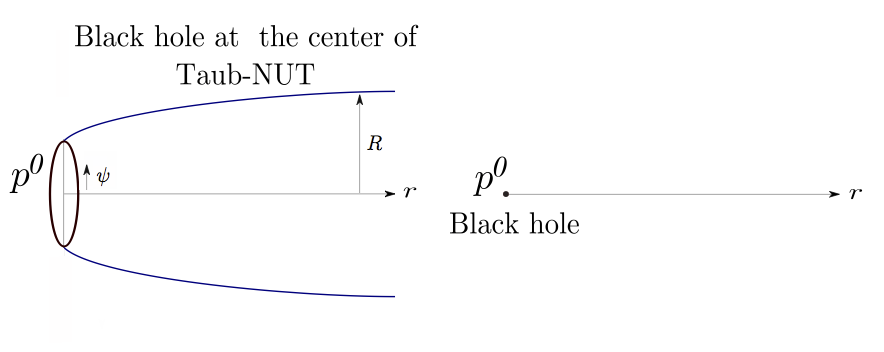
\includegraphics{Taub-NUT.png}
\caption{Dimensional reduction of a five-dimensional black hole (left) at the origin of a Taub-NUT space with Taub-NUT charge $p^{0}$ renders a four-dimensional black hole (right). From a four-dimensional perspective, the Taub-NUT charge is the magnetic charge of the black hole, associated with the graviphoton. This figure is adapted from \cite{Goldstein:2007kx}.}
\end{figure}

We will now review the procedure followed in \cite{Goldstein:2007kx} for a static black hole in five dimensions.

The five-dimensional theory considered contains $n_{v}$ vector fields $\hat{A}^{I}$ and $n_{s}$ real scalars $\hat{X}^{S}$ coupled to gravity and is described by the action\footnote{
In this section, five-dimensional quantities have a hat on top, whereas the four-dimensional ones go without.
}
\begin{equation}\label{goldstein-5D-action}
\begin{split}
\hat{\mathcal{S}} = \frac{1}{16\pi G_{5}} \int d^{5}x \sqrt{|\hat{g}|}
\Big( \hat{R} - \hat{h}_{ST}\partial_{\hat{\mu}}\hat{X}^{S}\partial^{\hat{\mu}}\hat{X}^{T} 
- \hat{f}_{IJ}\hat{F}^{I}_{\hat{\mu}\hat{\nu}} \hat{F}^{J\hat{\mu}\hat{\nu}}\\
- \hat{C}_{IJK} \frac{\epsilon^{\hat{\mu}\hat{\nu}\hat{\alpha}\hat{\beta}\hat{\gamma}}}{\sqrt{|\hat{g}|}} 
\hat{F}^{I}_{\hat{\mu}\hat{\nu}}\hat{F}^{J}_{\hat{\alpha}\hat{\beta}}\hat{A}^{K}_{\hat{\gamma}}
\Big).
\end{split}
\end{equation}

As usual upon dimensional reduction, the different fields are assumed to be independent of the fifth compact direction $\psi$. The standard relations between five- and four-dimensional fields are taken (see e.g.\ \cite{PopeKK})
\begin{equation}\label{KK-Ansatz}
\begin{split}
ds^{2}_{5} &= \omega^{-1}ds^{2}_{4} + \omega^{2}(d\psi + A^{0}_{\mu}dx^{\mu})^{2},\\
\hat{A}^{I} &= A^{I}_{\mu}dx^{\mu} + a^{I}(x^{\mu})(d\psi + A^{0}_{\mu}dx^{\mu}),\\
\hat{X}^{S} &= X^{S}(x^{\mu}).
\end{split}
\end{equation}
All the fields are functions of the non-compact directions $x^{\mu}$. This is shown explicitly for the axions $a^{I}$ to emphasize the a-priori non-constancy of them. We have stressed this, since it will be a point of discussion further on in this chapter.

Using these relations, dimensional reduction is performed along the compact $\psi$-direction such that the five-dimensional action \eqref{goldstein-5D-action} from a four-dimensional perspective reads (see e.g.\ \cite{Goldstein:2007kx})
\begin{equation}\label{goldstein-4D-action}
\mathcal{S} = \frac{1}{16\pi G_{4}} \int d^{4}x \sqrt{|g|}
\left( R - h_{st}\partial_{\mu}\varphi^{s}\partial^{\mu}\varphi^{t} - f_{ij}F^{i}_{\mu\nu}F^{j\mu\nu}
- \frac{1}{2} \tilde{f}_{ij} \frac{ \epsilon^{\mu\nu\alpha\beta}}{\sqrt{|g|}} F^{i}_{\mu\nu} F^{j}_{\alpha\beta}
\right).
\end{equation}
The real scalar fields $\varphi^{s}$ in four dimensions are the set of scalar fields $\{ \omega,a^{I},X^{S} \}$ in five dimensions $(s = 1 \ldots 1 + n_{v}+n_{s})$. Since the theory considered is not assumed to be supersymmetric, there is a-priori no relation between $n_{v}$ and $n_{s}$ and the descended scalar fields generically cannot be recast into complex combinations, unlike e.g.\  \cite{Cardoso:2007vn}. From the four-dimensional perspective, there is one gauge field more than in the five-dimensional theory. This extra gauge field, the graviphoton $A^{0}$, comes from the five-dimensional metric, and the set of four-dimensional gauge field strengths is given by $F^{i} = \{dA^{0},dA^{I}\}$ $(i = 0 \ldots n_{v})$. The exact content of the matrices $h_{st}$, $f_{ij}$ and $\tilde{f}_{ij}$, which depends on the content of the couplings in \eqref{goldstein-5D-action}, can be found in the original work, i.e.\ \cite{Goldstein:2007kx}.

Until now we considered a rather general five-dimensional theory with Chern-Simons terms, which was dimensionally reduced to an effective four-dimensional description of the theory.
Since we are interested in five-dimensional black holes, we must be sure that the dimensionally reduced theory also has black hole solutions. Otherwise, there were nothing to apply the entropy function formalism to. It turns out that it is not trivial that five-dimensional black hole solutions will descend to black holes in four dimensions. However, as discussed above there is a connection between static extremal black holes sitting in a five-dimensional Taub-NUT space with an $AdS_{2} \times S^{2} \times S^{1}$ near horizon symmetry,\footnote{In fact, static spherically symmetric extremal black holes in five dimensions have an $AdS_{2} \times S^{3}$ near horizon geometry.
The 3-sphere $S^{3}$ has locally a direct product structure of $S^{2} \times S^{1}$ and since the equations of motion do not use information about topology, one can as well use an $AdS_{2} \times S^{2} \times S^{1}$ near horizon geometry. It is shown in in \cite{Goldstein:2007kx} that one ultimately recovers $AdS_{2} \times S^{3}$ through a Hopf-fibration of the $S^{1}$ over the $S^{2}$, when the equations of motion are solved.}
and static spherically symmetric extremal black holes with an $AdS_{2} \times S^{2}$ near horizon geometry in four dimensions. 
This relation is used to define an entropy function for the five-dimensional black holes by identifying it with the entropy function for the associated four-dimensional black holes. This can be done, since the four-dimensional theory has no explicit appearance of gauge potentials in the action, as can be seen in \eqref{goldstein-4D-action}. For the four-dimensional black hole solutions then, Sen's formalism is well defined.

We thus consider five-dimensional black holes sitting in a Taub-NUT space with an $AdS_{2} \times S^{2} \times S^{1}$ near horizon geometry, such that the Kaluza-Klein Ansatz for all near horizon fields is specified to be
\begin{equation}\label{goldstein-KK-BH}
\begin{split}
ds_{5}^{2} &= \omega^{-1} \left[ v_{1}\left( -r^{2}dt^{2} + \frac{dr^{2}}{r^{2}} \right) + v_{2} (d\theta^{2} + \sin^{2}\theta d\phi^{2}) \right]
+ \omega^{2} (d\psi + p^{0}\cos\theta d\phi)^{2}, \\
\hat{A}^{I} &= \underbrace{e^{I}rdt + p^{I}\cos\theta d\phi}_\text{$A^{I}$} 
+ a^{I} (d\psi + \underbrace{p^{0}\cos\theta d\phi}_\text{$A^{0}$}), \\
\hat{X}^{S} &= u^{S}.
\end{split}
\end{equation}
Here $S^{2}$ is parametrized as usual, by $\theta = [0\ldots\pi[$ and $\phi = [0\ldots 2\pi[$, whereas $\psi$ has a periodicity of $4\pi$. All the fields are assumed to be constant along the horizon because of the spherical symmetry of the solutions sought after.

Now that we have an explicit relation between five- and four-dimensional black hole solutions, the entropy function for the five-dimensional black hole can be defined by identifying it with the entropy function of the associated four-dimensional black hole. This four-dimensional entropy function is the Legendre transform of the reduced Lagrangian with respect to the four-dimensional electric fields and their conjugate charges. Remember from \eqref{sen:reducedLag-def} on pg.\ \pageref{sen:reducedLag-def} that the reduced Lagrangian is the evaluation of the integral \eqref{goldstein-4D-action} along the horizon of the black hole. Let us make this concrete. The reduced four-dimensional Lagrangian is given by
\begin{equation}\label{GJ-defRL}
\mathcal{F}  = \frac{1}{16\pi G_{4}}\int d\theta\, d\phi \sqrt{|g|} \mathcal{L}
= \frac{1}{16\pi}\left(\frac{4\pi}{G_{5}}\int d\theta\, d\phi  \sqrt{|g|} \mathcal{L}\right),
\end{equation}
where we used that
\begin{equation}
\int d\psi \, G_{4} = G_{5}
\end{equation}
and $\sqrt{|g|} \mathcal{L}$ is the integrand in the action \eqref{goldstein-4D-action}, i.e.\ the dimensionally reduced one.
The physical values of the different fields near the horizon are then determined by their equations of motion\footnote{These are no real equations of motion as discussed in section \ref{sec:senEntropyFunc} on pg.\ \pageref{sec:senEntropyFunc}. Rather they give the values of the on-shell fields at the horizon.}
\begin{gather}\label{goldstein-eom1.1}
\frac{\partial \mathcal{F}}{\partial v_{i}} = \frac{\partial \mathcal{F}}{\partial \omega} = 
\frac{\partial \mathcal{F}}{\partial a^{I}} = \frac{\partial \mathcal{F}}{\partial u^{S}} =  0,\\
\label{goldstein-eom1.2}
\frac{\partial \mathcal{F}}{\partial e^{I}} = Nq^{I},
\end{gather}
where the normalization $N = 4\pi/ G_{5}$ is chosen. The entropy function for the five-dimensional black hole is then defined through
\begin{equation}\label{GJ-entrfuncDef}
\mathcal{E}_{5} \equiv \mathcal{E} = 2\pi(Nq_{I}e^{I} - \mathcal{F}).
\end{equation}
The equations of motion for the near horizon fields are then equivalent to
\begin{equation}\label{goldstein-eom2}
\frac{\partial \mathcal{E}}{\partial v_{i}} = \frac{\partial \mathcal{E}}{\partial \omega} = 
\frac{\partial \mathcal{E}}{\partial a^{I}} = \frac{\partial \mathcal{E}}{\partial u^{S}} = 
\frac{\partial \mathcal{E}}{\partial e^{I}} = 0,
\end{equation}
where it should be emphasized that the charges $q^{I}$ should be considered as fundamental upon partial differentiation, such that extremization does not pick up possible terms through the charges. If this were not the case, \eqref{goldstein-eom1.1}-\eqref{goldstein-eom1.2} and \eqref{goldstein-eom2} would not render equivalent sets of equations.\newline

The reduced Lagrangian, evaluated for the given background \eqref{goldstein-KK-BH}, gives \cite{Goldstein:2007kx}
\begin{multline}\label{goldstein-reducedLag}
\mathcal{F} = \left(
\frac{2\pi}{G_{5}} \right)\Bigg[ v_{1} -v_{2}
- \frac{v_{1}}{v_{2}}\left( \frac{\omega^{3}}{4}(p^{0})^{2}
+ \omega \hat{f}_{IJ}(p^{I} + p^{0}a^{I})(p^{J} + p^{0}a^{J}) \right)\\
+ \frac{v_{2}}{v_{1}} \omega\hat{f}_{IJ} e^{I}e^{J} \Bigg]
+ \left( \frac{24\pi}{G_{5}} \right) \hat{C}_{IJK} \big[ ( p^{I} + \frac{1}{2}p^{0}a^{I}) e^{J}a^{K} \big]
\end{multline}
From \eqref{goldstein-eom1.2} we find for the electric charges
\begin{equation}
q_{I} = \frac{v_{2}}{v_{1}}\omega \hat{f}_{IJ}e^{J} + 6 \hat{C}_{IJK} a^{K}(p^{J} + \frac{1}{2}p^{0}a^{J}).
\end{equation} 
The second term is a contribution originating in the Chern-Simons terms from the original five-dimensional action. We thus see that the Chern-Simons terms manifest themselves, after dimensional reduction, as a shift in the four\hyp{}dimensional charges $q^{I}$. Still, we have to bring the axions $a^{I}$ on-shell by extremizing \eqref{goldstein-reducedLag}. Doing so, one finds
\begin{equation}\label{GJ:eomAxions}
(- \frac{v_{1}}{v_{2}}\omega\hat{f}_{IJ} p^{0} + 6\hat{C}_{IJK}e^{K})(p^{J}+p^{0}a^{J})  = 0.
\end{equation}
This implies that the axions are given by
\begin{equation}
a^{I} = -\frac{p^{I}}{p^{0}},
\end{equation}
such that the charges upon substitution of the on-shell axion values are given by
\begin{equation}\label{GJ:onshellCharge}
q_{I} = \frac{v_{2}}{v_{1}}\omega \hat{f}_{IJ}e^{J} - 3 \hat{C}_{IJK} \frac{p^{J}p^{K}}{p^{0}}.
\end{equation}

We now turn our attention to the entropy of the black hole. Therefore we write down the entropy function \eqref{GJ-entrfuncDef}, with the on-shell axions already substituted,\footnote{
Note that the full entropy function, as defined in \eqref{GJ-entrfuncDef}, contains the \emph{off-shell} axions. Since we are ultimately interested in the entropy function evaluated for \emph{all} fields on-shell, we do not write down the full entropy function.
}
\begin{equation}\label{GJ:entropyFunc}
\mathcal{E} = \frac{4\pi^{2}}{G_{5}}\left(
v_{2} - v_{1} + \frac{v_{2}}{v_{1}}\omega \hat{f}_{IJ} e^{I} e^{J}
+ \frac{v_{1}}{v_{2}} \frac{\omega^{3}}{4} \big( p^{0} \big)^{2}
\right).
\end{equation}

Since we want to calculate the entropy of the black hole, we still need to bring the parameters $v_{1}, v_{2}$ and $\omega$ on-shell. It is fairly simply found that the radii of the metric are equal,
\begin{equation}\label{GJ:eomRadii}
v_{1} = v_{2}.
\end{equation}

Furtermore, the equation of motion for $\omega$ is given by
\begin{equation}
\frac{3}{4}\omega^{2}  \big( p^{0} \big)^{2} - \hat{f}_{IJ} e^{I} e^{J} = 0,
\end{equation}
which can be rewritten by defining the \emph{shifted} charges $\hat{q}_{I}$. These are defined from \eqref{GJ:onshellCharge} by
\begin{equation}\label{GJ:hattedCharge}
\hat{q}_{I} \equiv q_{I} + 3 \hat{C}_{IJK} \frac{p^{J}p^{K}}{p^{0}} = \frac{v_{2}}{v_{1}}\omega \hat{f}_{IJ}e^{J}.
\end{equation}
Using the on-shell values for $v_{1,2}$ and taking $\hat{f}^{IJ}$ to be the inverse of $\hat{f}_{IJ}$, it follows that
\begin{equation}
e^{I} = \omega^{-1} \hat{f}^{IJ} \hat{q}_{J}.
\end{equation}
We then find from its equation of motion that $\omega$ satisfies
\begin{equation}\label{GJ:eomOmega}
\omega^{4} = \frac{4}{3} \big( p^{0} \big)^{-2} \hat{f}^{IJ} \hat{q}_{I} \hat{q}_{J}.
\end{equation}
Substituting \eqref{GJ:eomRadii} and \eqref{GJ:eomOmega} in \eqref{GJ:entropyFunc}, we find the entropy of the five\hyp{}dimensional black hole, namely
\begin{equation}\label{GJ:entropyBH}
S = \frac{4\pi^{2}}{G_{5}} \sqrt{p^{0}\left( \frac{4}{3} \hat{f}^{IJ} \hat{q}_{I} \hat{q}_{J} \right)^{3/2}}.
\end{equation}


%----------------------------------------------
%SECTION
%----------------------------------------------
\section{Intermezzo: Maxwell charge vs.\ Page charge}
\label{sec:intermezzoCharges}

In this section we point out that the presence of Chern-Simons terms in five-dimensional theories leads to different notions of charge, associated with the gauge fields. The entropy function is defined as the Legendre transform with respect to the electric fields, conjugate to some charges. When defining an entropy function in five dimensions in the next section, we will be confronted with the ambiguity in choosing the right charges conjugate to the fields. Therefore we recall how this ambiguity arises in the presence of Chern-Simons terms.  It was summarized in \cite{Marolf:2000cb} that there are at least three different natural choices of charge associated with the Abelian gauge fields. Here, two of them will be discussed, namely Maxwell charge and Page charge. The third one reviewed in \cite{Marolf:2000cb}, brane source charge, was originally discussed in \cite{Bachas:fk}. 

Consider the five-dimensional $N=2$ supergravity action \eqref{eq:actionN2D5}, which implies the following equations of motion for the gauge fields $A^{I}$,
\begin{equation}
G_{IJ}d\star F^{J} + \frac{1}{4} C_{IJK} F^{J} \wedge F^{K} = 0.
\end{equation}
For simplicity, we will discuss the case when there is only one gauge field in the theory, such that its vacuum equation of motion is
\begin{equation}\label{eq:eomGauge5D}
d\star F + \frac{1}{4}F \wedge F = 0.
\end{equation}

\paragraph{Maxwell charge}

The equation of motion \eqref{eq:eomGauge5D} can be rewritten in the form
\begin{equation}
d\star F = \star j^{\mathrm{Maxwell}}, \qquad  \star j^{\mathrm{Maxwell}} \equiv -\frac{1}{4}F \wedge F,
\end{equation}
where the idea is used that any term sourcing the gauge field equations of motion should be interpreted as a Maxwell charge. Of course, when we consider also source terms in \eqref{eq:eomGauge5D}, these should also be added in the Maxwell current.\footnote{
These extra source terms will be what we call in the next paragraph, the Page current.}
One sees that, although the gauge fields considered are Abelian, they do carry charge, as analogous to the non-Abelian gauge fields appearing in Yang-Mills theories. From its definition it is manifest that the current is gauge invariant and conserved, since it is made up out of closed 2-forms. On the other hand, it is not localized, as the charge is carried by the fields themselves. Indeed, integrating $\star F$ over some boundary $\partial V$ of a volume $V$ gives the charge contained in that volume. However, since the charge is smeared out over space-time, it may be impossible to deform the boundary in such a way that the amount of measured charge is unchanged. This means that generically the total amount of Maxwell charge can be measured only at spatial infinity.

\paragraph{Page charge}

 This notion of charge was introduced first by Page \cite{Page:1983pc}. We again slightly rewrite \eqref{eq:eomGauge5D} as
\begin{equation}
d ( \star F + \frac{1}{4} A \wedge F ) = \star j^{\mathrm{Page}},
\end{equation}
where we introduced some localized amount of \emph{Page current}, sourcing the left-hand side in \eqref{eq:eomGauge5D}. Furthermore, this type of charge is conserved as implied by $d^{2} = 0$. Note however, that the Page charge
\begin{equation}\label{def:PageCharge}
q^{\mathrm{Page}} \equiv \int_{V} \star j^{\mathrm{Page}} = \int_{\partial V} (\star F + \frac{1}{4} A \wedge F)
\end{equation}
is gauge dependent under large gauge transformations. Small gauge transformations pose no problem, since a boundary has no boundary. What is meant by this is, that after performing a small gauge transformation $A \rightarrow A + d\lambda$ the Page charge goes as
\begin{equation}
q^{\mathrm{Page}} \rightarrow q^{\mathrm{Page}} + \frac{1}{4} \int_{\partial V} d\big( \lambda \wedge F \big).
\end{equation}
Since $\partial V$ is a boundary, it has no boundary and Stokes' theorem implies that the integral is zero. Hence the Page charge is invariant under small gauge transformations.\\

From their definitions we have a relation between Maxwell and Page charge, i.e.\
\begin{equation}
q^{\mathrm{Maxwell}} = q^{\mathrm{Page}} - \int_{\partial V} A \wedge F,
\end{equation}
which implies that at spatial infinity Maxwell and Page charges are measured to be equal, assuming the vanishing of the gauge fields at infinity.
 
%----------------------------------------------
%SECTION
%----------------------------------------------
\section{Systematic five-dimensional procedure}

In this section we review the approach followed in \cite{Arsiwalla:2008gc}. There it is proposed that it is possible to have a consistent definition of the entropy function in the presence of Chern-Simons terms, without taking recourse to a dimensional reduction. A crucial point will turn out to be the right choice of charges, conjugate to the electric fields. As we reviewed in the previous section, different choices of charge are possible in five dimensions and a-priori it might not be clear, which one should be used in the entropy function formalism. As we will review shortly, the charge defined in \cite{Arsiwalla:2008gc} is suggested to be Page charge. There is a good reason to believe that Page charge is the natural choice of charge, as it is measurable at the horizon as opposed to Maxwell charge. An entropy depending on the latter would need asymptotic information, which is undesirable for a microscopic interpretation of the macroscopic entropy. We find however that there is a small mismatch between the charge defined in \cite{Arsiwalla:2008gc} and the Page charge associated with the theory considered. This mismatch stems from the way in which the charge is defined and is rooted in the explicit appearance of the gauge potentials in the action describing the theory.

It was mentioned in \cite{Arsiwalla:2008gc} that the entropy of a static spherically symmetric extremal black hole computed there, differed from the entropy computed in \cite{Goldstein:2007kx} for the same black hole configuration through dimensional reduction. However, we show that these entropies are in exact agreement. Instead, we do not confirm some of the intermediate results found in the proceedings of the direct five-dimensional approach of \cite{Arsiwalla:2008gc}. Let us now review this in detail, postponing a discussion regarding these issues to the next section.\\

The setting considered in \cite{Arsiwalla:2008gc} is a five-dimensional theory with Chern-Simons terms, more specifically the bosonic sector of $N=2$ supergravity, see section \ref{N2D5Sugra}, pg.\ \pageref{N2D5Sugra}, i.e.\footnote{
The matrix $G_{IJ}$ used here, equals $2\hat{f}_{IJ}$ in \eqref{goldstein-5D-action}. The factor 1 in front of the Chern-Simons terms is chosen to have the same normalization as in \cite{Arsiwalla:2008gc}.
}
\begin{equation}\label{eq:actionN2D5-bis}
\mathcal{S}_{5} = \frac{1}{16\pi G_{5}} \int R\star 1 - G_{IJ}dX^{I}\wedge\star dX^{J} - G_{IJ}F^{I}\wedge\star F^{J}-
C_{IJK}F^{I}\wedge F^{J}\wedge A^{K}.
\end{equation}
The notation here differs slightly from the one in the action \eqref{goldstein-5D-action}, used in the first section of this chapter. We do not use hats on top of the quantities, since we will only work in five dimensions, whereas the hats in \eqref{goldstein-5D-action} were used to make the distinction clear between five-dimensional quantities and the dimensionally reduced four-dimensional ones. Furthermore, the number of real scalar fields and gauge fields is the same, as is the case for the bosonic part of five-dimensional supergravity theories, see section \eqref{N2D5Sugra}, pg.\ \pageref{N2D5Sugra}. The following discussion however does not rely on any supersymmetry arguments, and we could have considered a different number of scalar and gauge fields. Nonetheless we stick with the notation, since it connects better to the original work, i.e.\ \cite{Arsiwalla:2008gc}.

Because we want to compare this direct five-dimensional approach with the formalism through dimensional reduction, we take the same near horizon Ansatz as in section \ref{EF-CS-dimRed}, i.e.\ the one given in \eqref{goldstein-KK-BH}, pg.\ \pageref{goldstein-KK-BH}. We copy it here for convenience,
\begin{equation}\label{arsiwalla-BH}
\begin{split}
ds_{5}^{2} &= \omega^{-1} \left[ v_{1}\left( -r^{2}dt^{2} + \frac{dr^{2}}{r^{2}} \right) + v_{2} (d\theta^{2} + \sin^{2}\theta d\phi^{2}) \right]
+ \omega^{2} (d\psi + p^{0}\cos\theta d\phi)^{2}, \\
A^{I} &= e^{I}rdt + p^{I}\cos\theta d\phi + a^{I} (d\psi + p^{0}\cos\theta d\phi), \\
X^{S} &= u^{S}.
\end{split}
\end{equation}

The Chern-Simons terms in \eqref{eq:actionN2D5-bis} prevent us from applying Sen's formalism straightforwardly. As discussed in section \ref{sec:limSenFormalism} on pg.\ \pageref{sec:limSenFormalism}, the action is not invariant under large gauge transformations. These large gauge transformations are implemented in the Ansatz \eqref{arsiwalla-BH} through \cite{Arsiwalla:2008gc}
\begin{equation}
a^{I} \rightarrow a^{I} + k^{I}.
\end{equation}
To keep track of this gauge ambiguity in the following discussion, the shifted axions $\tilde{a}^{I}$ are introduced through
\begin{equation}
\tilde{a}^{I} \equiv a^{I} + k^{I}.
\end{equation}

The reduced Lagrangian in five dimensions is defined analogously to the definition in four dimensions, i.e.\ by evaluating \eqref{eq:actionN2D5-bis} along the horizon of the black hole. We thus have
\begin{equation}
\mathcal{F} = \frac{1}{16\pi G_{5}} \int_{\mathrm{H}} d\theta\, d\phi \, d\psi \, \sqrt{|g|} \mathcal{L}.
\end{equation}
Computing this reduced Lagrangian for the Ansatz \eqref{arsiwalla-BH}, one finds \cite{Arsiwalla:2008gc}
\begin{multline}\label{arsiwalla-reducedLag}
\mathcal{F} = \left(
\frac{2\pi}{G_{5}} \right)\Bigg[ v_{1} -v_{2}
- \frac{v_{1}}{v_{2}}\left( \frac{\omega^{3}}{4}(p^{0})^{2}
+ \omega \frac{G_{IJ}}{2}(p^{I} + p^{0}\tilde{a}^{I})(p^{J} + p^{0}\tilde{a}^{J}) \right)\\
+ \frac{v_{2}}{v_{1}} \omega\frac{G_{IJ}}{2} e^{I}e^{J} \Bigg]
+ \left( \frac{24\pi}{G_{5}} \right) C_{IJK} \big[ ( p^{I} + \tilde{a}^{I}p^{0}) e^{J}\tilde{a}^{K} \big].
\end{multline}

Let us compare this expression with the one obtained in \eqref{goldstein-reducedLag} through dimensional reduction \cite{Goldstein:2007kx}. There are two differences to be noted. Firstly, as expected, the large gauge ambiguity appears through the shifted axions $\tilde{a}^{I}$ in \eqref{arsiwalla-reducedLag}. The second discrepancy between \eqref{arsiwalla-reducedLag} and \eqref{goldstein-reducedLag} is the factor $1/2$ in the Chern-Simons term of \eqref{goldstein-reducedLag}. As \cite{Arsiwalla:2008gc} suggests, this factor stems from the manner, in which axions are treated in \cite{Goldstein:2007kx}. In the latter, the axions are assumed to have a space-time dependence in the non-compact directions, see \eqref{KK-Ansatz}. Dimensional reduction is then performed, assuming this dependence, and the axions are set to constants only when one arrives at the effectively four-dimensional set-up, see \eqref{goldstein-KK-BH}. We have redone the dimensional reduction of the Chern-Simons term and the factor $1/2$ indeed follows from the space-time dependence of the axions. For the details of this reduction, we refer to appendix \ref{app:DR-CS-GJ}. In the next section we come back to this issue.\newline

The 5D charges $Q_{I}$, conjugate to the electric fields $e^{I}$ are defined through \cite{Arsiwalla:2008gc},
\begin{align}\label{XA:charges}
Q_{I} &\equiv \frac{G_{5}}{4\pi} \frac{\partial \mathcal{F}}{\partial e^{I}} \notag\\
&= \frac{v_{2}}{v_{1}} \omega \frac{G_{IJ}}{2} e^{J} + 6C_{IJK}(p^{J} + \tilde{a}^{J}p^{0})\tilde{a}^{K}.
\end{align}
As correctly concluded in \cite{Arsiwalla:2008gc}, these charges are given by
\begin{equation}\label{XA:charges2}
Q_{I} = \frac{1}{16\pi^{2}} \int_{H} G_{IJ} \star F^{J} + 6 C_{IJK} A^{J} \wedge F^{K} 
\end{equation}
evaluated for the Ansatz \eqref{arsiwalla-BH}.
Following \cite{Arsiwalla:2008gc}, it was suggested that these charges are Page charges. As we saw in the last section, Page charge seems indeed the natural choice of localized charge for supergravity theories, as was also studied in \cite{Hanaki:2007mb}. However, there is a small mismatch between the charges \eqref{XA:charges2} and the Page charges, as defined in \eqref{def:PageCharge}. The discrepancy is due to a mismatch in the factor in front of the second term. In the following it turns out that this term goes to zero at the horizon for the solutions considered here, once the fields are taken on-shell. This means that the discrepancy will have no physical implication here and will not influence the entropy of a static extremal black hole. Nonetheless, it may be of physical importance for a generic black hole solution and we discuss this issue in detail in the next section.

Once the charges are identified, the five-dimensional entropy function is defined as the Legendre transform of $\mathcal{F}$ with respect to these charges, i.e.\
\begin{equation}\label{XA:entrFunct-def}
\mathcal{E} = 2\pi \left( \frac{4\pi}{G_{5}} Q_{I}e^{I} - \mathcal{F} \right),
\end{equation}
such that the equations of motion of the different near horizon fields are given upon extremization of $\mathcal{E}$ with respect to the corresponding fields. Here, it should be stressed again that the charges are considered fundamental and thus independent of the fields, when the entropy function is differentiated. The reason is that extremizing the entropy function would otherwise give equations which are not equivalent to the equations of motion. The latter are defined by extremizing the reduced Lagrangian with respect to the near horizon values of the fields.\newline

The entropy of the black hole can be calculated by bringing the different fields on-shell near the horizon. It was stated in the procedure in \cite{Arsiwalla:2008gc} that,
\begin{equation}\label{XA:eomAxions}
\frac{\partial \mathcal{E}}{\partial a^{I}} = 0 \qquad \Longrightarrow \qquad p^{I} + \tilde{a}^{I} p^{0} = 0.
\end{equation}
This result was also concluded in the procedure followed by \cite{Goldstein:2007kx}, see \eqref{GJ:eomAxions} on pg.\ \pageref{GJ:eomAxions}. Moreover, this implies a vanishing magnetic flux since
\begin{equation}\label{XA:vanishMagFlux}
\int_{S^{2}} F^{I} = 4\pi \big( p^{I} + \tilde{a}^{I} p^{0} \big) = 0,
\end{equation}
where $S^{2}$ is a 2-sphere surrounding a point on the $S^{1}$, parametrized by $\psi$ \cite{Emparan:2004fk}.

It thus seems to be the right equation of motion. However, when calculating the variation of the entropy function with respect to the axions, we find
\begin{equation}\label{XA:realeomAxions}
\frac{\partial \mathcal{E}}{\partial a^{I}} = 
-\frac{v_{1}}{v_{2}} \omega \frac{G_{IJ}}{2} p^{0} \big( p^{J} + \tilde{a}^{J} p^{0} \big)
+ 6 C_{IJK} \big( p^{J} + 2 \tilde{a}^{J} p^{0} \big) e^{K} = 0.
\end{equation}
If this were to imply \eqref{XA:eomAxions}, it also implies the vanishing of $ p^{J} + 2 \tilde{a}^{J} p^{0}$ such that the $p^{J}$ and the $\tilde{a}^{J}$ vanish separately. This seems too big a constraint on the fields and we will see later that the vanishing of the magnetic flux can also be concluded by computing the equations of motion for the $\psi$-component of the gauge field. We believe that the latter are the correct equations of motion and as it turns out, they are not equivalent to extremizing $\mathcal{E}$ with respect to the axions. We will make this point concrete in the next section.

Nonetheless, since the vanishing of $p^{J} + \tilde{a}^{J} p^{0}$ seems to be the correct conclusion, we can use it as a further input for the charges \eqref{XA:charges}, such that they are given by
\begin{equation}
Q_{I} = \frac{v_{2}}{v_{1}} \omega \frac{G_{IJ}}{2} e^{J}.
\end{equation}
These charges are exactly the same as the four-dimensional shifted charges $\hat{q}_{I}$, obtained in \eqref{GJ:hattedCharge}. However, it should be remembered that the charges conjugate to the four-dimensional electric fields were given by the $q_{I}$ in \eqref{GJ:onshellCharge} and not by the $\hat{q}_{I}$, whereas in five dimensions, the conjugate charges are given by $Q_{I} = \hat{q}_{I}$.
Furthermore it should be noted that the Chern-Simons term in the reduced Lagrangian \eqref{arsiwalla-reducedLag} vanishes for the near horizon, when the fields are taken on-shell.

Using these results we calculate the entropy function \eqref{XA:entrFunct-def}, which is then found to be
\begin{equation}\label{XA:entropyFunc}
\mathcal{E} = \frac{4\pi^{2}}{G_{5}}\left(
v_{2} - v_{1} + \frac{v_{2}}{v_{1}}\omega \frac{G_{IJ}}{2} e^{I} e^{J}
+ \frac{v_{1}}{v_{2}} \frac{\omega^{3}}{4} \big( p^{0} \big)^{2}
\right).
\end{equation}
In analogy to the treatment in section \ref{EF-CS-dimRed} it is found that the metric radii are equal,
\begin{equation}
v_{1} = v_{2}
\end{equation}
when their equations of motion are calculated. Furthermore, we find that $\omega$ satisfies
\begin{equation}
\omega^{4} = \frac{4}{3} \big( p^{0} \big)^{-2} 2G^{IJ} Q_{I} Q_{J}.
\end{equation}
Evaluating the entropy function for the on-shell values implied by these relations renders the entropy of the black hole, namely
\begin{equation}\label{XA:entropy5D}
S = \frac{4\pi^{2}}{G_{5}} \sqrt{p^{0} \left( \frac{4}{3} 2G^{IJ} Q_{I} Q_{J} \right)^{3/2}}.
\end{equation}
This result is exactly the same as the entropy found through dimensional reduction in \eqref{GJ:entropyBH}, since $2G^{IJ} = \hat{f}^{IJ}$.

%----------------------------------------------
%SECTION
%----------------------------------------------
\section{Analysis}

In this last section we compare the two procedures presented above. As shown, both formalisms---dimensional reduction and direct five-dimensional approach---give the same entropy for the five-dimensional black holes considered. In \cite{Arsiwalla:2008gc} it was concluded that the two approaches resulted in different entropies and it was argued that the direct five-dimensional approach gave the correct result, since their entropy matched the one found in \cite{Larsen:2006xm}, computed via a five-dimensional attractor mechanism for BPS black holes. The entropy \eqref{GJ:entropyBH} however, calculated through a dimensional reduction, equals both the entropies in \cite{Arsiwalla:2008gc} and \cite{Larsen:2006xm} if the same coupling content in the theory is considered. Nonetheless, there seem to be some minor problems with the direct five-dimensional approach. First of all, the charges defined there are not in exact agreement with the Page charges in the theory. The reason is that extremization was done with respect to the field strengths, which for a theory with Chern-Simons terms does not result in the equations of motion of the gauge fields. Secondly, differentiating the entropy function with respect to the axions does not give the right equations of motion, as they are defined in Lagrangian mechanics. It turns out that this inequivalence is due to the Kaluza-Klein Ansatz.\newline

In the five-dimensional procedure the charges were defined in \eqref{XA:charges}, such that they were given by \eqref{XA:charges2},
\begin{equation}\label{XA:charges2bis}
Q_{I} \equiv \frac{G_{5}}{4\pi} \frac{\partial \mathcal{F}}{\partial e^{I}}
= \frac{1}{16\pi^{2}} \int_{\mathrm{H}} G_{IJ} \star F^{J} + 6 C_{IJK} A^{J} \wedge F^{K}.
\end{equation}
These charges are not the Page charges, since the latter ones are defined through the equations of motion, which follow from the action \eqref{eq:actionN2D5-bis}. These equations of motion are given by
\begin{equation}
d \big( G_{IJ} \star F^{J} + \frac{3}{2} C_{IJK} A^{J} \wedge F^{K} \big) = \star j^{\mathrm{Page}}, 
\end{equation}
such that the Page charge equals (see \eqref{def:PageCharge})
\begin{equation}\label{XA:PageCharges}
Q_{I}^{\mathrm{Page}} = \frac{1}{16\pi^{2}} \int_{\mathrm{H}} G_{IJ} \star F^{J} + \frac{3}{2} C_{IJK} A^{J} \wedge F^{K}. 
\end{equation}
The discrepancy in the factor in front of the second term, which stems from the Chern-Simons term, is due to the fact that in the definition of the charges \eqref{XA:charges2}, the reduced Lagrangian was differentiated with respect to a field strength component. In a theory where there appear no gauge fields explicitly in the action, the gauge field equations of motion can indeed be found by considering the gauge field strengths as fundamental, rather than the gauge fields themselves. What is meant by this, is that for such a theory, the equations obtained by
$
d \big( \delta \mathcal{S} / \delta F \big) = 0$ and $\delta \mathcal{S} / \delta A = 0
$
render the same equations of motion.\footnote{Actually, one should explicitly add the Bianchi-identity $dF = 0$ to the equations of motion if $F$ is taken to be fundamental. This is needed, since if $A$ were to be taken fundamental, this identity would follow directly from the closure of an exact form.
} This can be understood as follows. Consider an action where the gauge potentials appear only through their associated field strengths. Differentiating the action then gives ($F = dA$),
\begin{equation}
\delta \mathcal{S}[dA] = \frac{\delta \mathcal{S}}{\delta(dA)} \delta(dA)
\sim d\frac{\delta \mathcal{S}}{\delta F} \delta A,
\end{equation}
where we used integration by parts in the last step.
This is the reason why in the original work of Sen, the near horizon equations of motion for the gauge fields were given by \eqref{eq:eomNHGaugeSen}, where the Lagrangian was varied with respect to the electric fields. However, when there are gauge fields appearing explicitly in the Lagrangian, one should check first if the equations obtained by extremizing with respect to the gauge field strengths, renders the same equations as the ones obtained where the action was extremized with respect to the gauge fields. This is not the case for the theory considered here, and the discrepancy in factors between \eqref{XA:charges2bis} and \eqref{XA:PageCharges} is due to the non-equivalence of these equations of motion. 
We thus see that the charges \eqref{XA:charges} are not Page charges and in fact they seem to be even non-conserved quantities. This is suggested because in the presence of Chern-Simons terms the equation
\begin{equation}\label{conservedCharge1}
Q_{I} = N \frac{\partial \mathcal{F}}{\partial e^{I}}
\end{equation}
with $Q_{I}$ a set of conserved charges, does not make any sense since it is based on the observation that for an action with no explicit appearance of gauge potentials
\begin{equation}
\frac{\delta \mathcal{S}}{\delta A} \sim d \frac{\delta \mathcal{S}}{\delta F} = \star j_{I},
\end{equation}
where $j_{I}$ is some localized current in the black hole. It is the integration of this equation along the near horizon of a spherical symmetric extremal black hole, which would give us \eqref{conservedCharge1}.

The noted discrepancy will turn out to be irrelevant, when calculating the entropy of the static black hole we consider here. This is so, because the equations \eqref{XA:eomAxions} imply that the second term in the Page charge is zero. Since the difference between the two charges is due to the second term, the charges \eqref{XA:charges2bis} equal the Page charges, once the equations of motion are taken into account. It is because of this ``on-shell equality'' of the charges that there is no discrepancy on the level of the entropy, since the latter is the evaluation of the entropy function for all the near horizon values of the fields on-shell. Nonetheless, when considering the entropy function \eqref{XA:entrFunct-def}, all fields are still off-shell such that using different charges gives non-equivalent results.

To conclude this comment on the choice of charge we argue why Page charge seems the right quantity to use in a five-dimensional entropy function formalism. 
Remember that the entropy function in four dimensions encodes the attractor mechanism, as the entropy turns out to be determined by local information alone. Indeed, since the Maxwell current in four dimensions is localized in the black hole, the associated charges can be measured at the horizon. If the entropy function in five dimensions wants to encode an attractor mechanism too, it seems natural to have it depending on Page charge whenever Chern-Simons term do play a role for the background. This is so because the associated Page current is divergenceless outside the black hole, as opposed to the Maxwell current in the presence of Chern-Simons terms (see section \ref{sec:intermezzoCharges} on pg.\ \pageref{sec:intermezzoCharges}). As such, Page charge, although defined at spatial infinity, is measurable at the black hole horizon. Because of this local property, macroscopic entropy in terms of Page charge has the possibility to be given a statistical interpretation.\newline

We now focus a bit more on the result that the magnetic flux vanishes, i.e.\
\begin{equation}\label{XA:eomAxionsBis}
p^{I} + \tilde{a}^{I} p^{0} = 0.
\end{equation}
This result was derived in \cite{Arsiwalla:2008gc} by extremizing the entropy function, or equivalently the reduced Lagrangian, with respect to the axions $a^{I}$, see \eqref{XA:eomAxions}. However, extremizing the reduced Lagrangian with respect to the axions gives \eqref{XA:realeomAxions}, which was a too strong constraint on the fields, since this implied both the vanishing $p^{I}$ and $\tilde{a}^{I} p^{0}$. We show that the equations \eqref{XA:eomAxionsBis} are in fact the equations of motion of $A^{I}_{\psi}$. Indeed, it follows from the action \eqref{eq:actionN2D5-bis} that the gauge fields satisfy
\begin{equation}
\partial_{\mu} \left( \sqrt{|g|} \,G_{IJ} F^{\mu\nu J} \right) + \frac{3}{8}
C_{IJK} F^{J}_{\mu\tau} F^{K}_{\rho\sigma} \epsilon^{\mu\tau\rho\sigma\nu} = 0.
\end{equation}
Evaluating the $\psi$-component, i.e.\ $\nu = \psi$, for the near horizon Ansatz \eqref{arsiwalla-BH} gives the following expression,
\begin{equation}
(- \frac{v_{1}}{v_{2}} \omega G_{IJ} p^{0} + 3 C_{IJK} e^{K}) (p^{J} + a^{J} p^{0} ) \sin\theta  = 0,
\end{equation}
which indeed implies \eqref{XA:eomAxionsBis}. Since in the Ansatz \eqref{arsiwalla-BH} $A^{I}_{\psi}$ is $a^{I}$, one could wonder why we do not find the right equations of motion when the reduced Lagrangian is extremized with respect to the $a^{I}$. The reason lies in the fact that the axions also appear in the other components of the gauge fields due to the Kaluza-Klein Ansatz \eqref{arsiwalla-BH}. When the reduced Lagrangian, or for that matter, the entropy function is extremized, extra terms because of these other components are picked up.

As we mentioned before, it was concluded in \cite{Arsiwalla:2008gc} that the entropies \eqref{GJ:entropyBH} and \eqref{XA:entropy5D} do not match. It was already shown in this chapter, that the entropies are the same. However, we for the moment consider the discrepancy mentioned in \cite{Arsiwalla:2008gc}, since we want to elaborate somewhat more on their conclusions regarding this mismatch. There it was suggested that the apparent discrepancy in entropies was due to the way in which the axions were treated in \cite{Goldstein:2007kx}. In the latter the axions are assumed to be space-time dependent when dimensionally reducing the five-dimensional theory and are only set to constants in the near horizon Ansatz of the effective four-dimensional description. This would lead to an erroneous shift in the charges, due to a factor of $1/2$ coming from the dimensional reduction of the Chern-Simons terms (see appendix \ref{app:axions(x)}, where we have redone this reduction. The factor $1/2$ can be seen in the second term, coming from the original Chern-Simons term, in eq.\ \eqref{eq:axions(x)}). The entropy function would pick up this factor $1/2$, implying a wrong entropy of the black hole. It was proposed in \cite{Arsiwalla:2008gc} that the axions should be treated as constants in the five-dimensional theory before performing a dimensional reduction. We do not confirm this reasoning, since we believe the axions are space-time dependent---at least in the non-compact directions---in the full five-dimensional theory. Dimensional reduction of the black hole solution is performed for the whole space-time, not only for the near horizon geometry, so that at this stage the axions should be taken non-constant. Also, assuming less symmetry in a problem should at most make things more difficult, but not lead to wrong answers when considering the symmetry at a later stage in the process of solving the problem. Furthermore, we have done a dimensional reduction of the Chern-Simons term, considering the axions space-time dependent, see appendix \ref{app:axions}, and the factor 1/2 indeed disappears as can be seen in eq. \eqref{eq:axions}. Imagine now that \eqref{eq:axions} were to be used as the contribution coming from the Chern-Simons terms in the reduced Lagrangian \eqref{goldstein-reducedLag}, instead of \eqref{eq:axions(x)}. In that case we would not find a vanishing magnetic flux \eqref{GJ:eomAxions}. This suggests that the axions should not be put to constants in five dimensions. Having said this, we emphasize again that the entropies do match. We believed however that the question regarding the possible (non-)\linebreak[0]constancy of the axions was worth discussing, since we may conclude that the approach using dimensional reduction is consistent. 

That the entropies computed in both procedures turn out to be the same is with hindsight not too difficult to understand. Once the axions are taken on-shell, the Chern-Simons terms do not play a role in the entropy functions \eqref{GJ:entropyFunc} and \eqref{XA:entropyFunc}, which equal each other. In the procedure via dimensional reduction, this disappearance of the Chern-Simons terms is a subtle cancellation between the on-shell charges and the on-shell Chern-Simons term in the reduced Lagrangian, where the factor 1/2 is crucial. In the direct approach, the cancellation is a direct consequence of the vanishing of the magnetic flux. Since the Chern-Simons terms vanish explicitly in five dimensions, the entropy function formalism is well-defined once the axions are on-shell. We believe it is a test of consistency of the procedure via dimensional reduction, that it equals the entropy calculated in five dimensions, since in four dimensions the Chern-Simons terms are not put trivially to zero, once the axions are on-shell. Rather they disappear through the above mentioned cancellation.\newline

To conclude this analysis, we comment on the already discussed issue of large gauge transformations. In \cite{Arsiwalla:2008gc}, the fact that theories containing Chern-Simons terms are not invariant under large gauge transformations was identified as the source of the problem in applying Sen's entropy function formalism. However, we believe that this non-invariance of the action is not as problematic as it may seem. It is true that Sen's original formalism was developed on the assumption of gauge invariance of the considered theories. However, actions containing Chern-Simons terms are invariant under small gauge transformation and this seems to be sufficient. In classical electrodynamics the issue of small and large gauge transformations also pops up. Consider the interaction term that couples a current $j$ to a gauge field $A$, i.e.\ \begin{equation}\int \star j \wedge A. \end{equation}
It is well known that demanding global $U(1)$ invariance of the action implies a conserved current, the argument being
\begin{equation}
\int \star j \wedge A \rightarrow \int \star j \wedge (A + d\lambda) = \int \star j \wedge A - \int d \star j \wedge \lambda.
\end{equation}
As the second term should be zero, we have a conserved current $d \star j = 0$ for small gauge transformations $\Lambda = d\lambda$. This argument breaks down when the gauge transformations are large, since these are not exact forms. Hence, it seems that only small gauge transformations are considered when discussing the gauge invariance of a theory.\newline

\noindent
Some of the issues regarding a direct five-dimensional approach we discussed above were suggested by studying a spherically symmetric extremal black hole with an $AdS_{2} \times S^{3}$ near horizon geometry. Including this in the main text would lead to a repetition of what is said in the last two sections. Nonetheless, as it was of inspiration to some conclusions drawn in these sections, we have put the results in the appendix. They can be found in appendix \ref{inspirationDirect5D}.

\newpage
\thispagestyle{empty}
%----------------------------------------------
%-----------------
%CHAPTER
%-----------------
%----------------------------------------------
\chapter{Discussion and outlook}

In this thesis we compared two possible definitions of an entropy function formalism in theories of gravity coupled to a number of scalar and gauge fields in five dimensions in the presence of gauge Chern-Simons terms. One of the hurdles to be taken in extending the formalism is due to the explicit appearance of the gauge potentials in the Chern-Simons terms. We have investigated two proposals, i.e.\ through dimensional reduction and a systematic five dimensional procedure, for the case of a static spherically symmetric extremal black hole. Doing so, we have demonstrated and analyzed the differences between these procedures.

The first approach is consistent since it identifies the entropy function in five dimensions with the entropy function in four dimensions, which is well defined for the four-dimensional black holes, connected to the five-dimensional ones. A disadvantage of the procedure using dimensional reduction is, that it is only applicable to five-dimensional black holes that can be related to four-dimensional black hole solutions. A question towards the future could be, how this approach can be extended to five-dimensional black holes, not residing in an asymptotic Taub-NUT space.

When trying to define an entropy function directly in five dimensions analogous to its definition in four dimensions, we encountered some problems. First of all, because of the different notions of charge in theories with Chern-Simons terms, there is an ambiguity which quantity is the correct one to use in an entropy function formalism. We argued that this should be the Page charge as it is localized and hence allows for a formalism that implies the attractor mechanism at work for the black hole. However, we have seen that the Page charge is in general not a conjugate quantity to the electric field, because the gauge fields appear explicitly in the action. Therefore, how to consistently define an entropy function as a Legendre transform in five dimensions remains unclear to us, and we believe it certainly is an interesting question to be answered.






%--------------------------------------------------------
%Appendices
%--------------------------------------------------------

\begin{appendices}

%Head style appendix
%------------------------------------
\renewcommand{\chaptermark}[1]{%
\markboth{Appendix%
\ \thechapter.%
\ #1}{}}

\renewcommand{\sectionmark}[1]{%
\markright{
\thesection%
\ #1}{}}

\fancyhead{} % clear all header fields
\fancyhead[RO,LE]{\thepage}
\fancyhead[RE]{\leftmark}
\fancyhead[LO]{\rightmark}
\fancyfoot{} % clear all footer fields
\renewcommand{\headrulewidth}{0.4pt}
%------------------------------------


%----------------------------------------------
%-----------------
%APPENDIX
%-----------------
%----------------------------------------------
\chapter{Conventions and notation}

%----------------------------------------------
%SECTION
%----------------------------------------------
In this text, we mostly use the convention
\begin{equation}
c = \hbar = k_{\mathrm{B}} = G_{\mathrm{N}} =1,
\end{equation}
however sometimes restoring a constant, especially Newton's constant $G_{\mathrm{N}}$.
The space-time metric has a Lorentzian signature $(-,+,+,+)$ in four dimensions and $(-,+,+,+,+)$ in five dimensions.


%----------------------------------------------
%SECTION
%----------------------------------------------
\section{Levi-Civita symbol}\label{App:LC-symbol}

We define the Levi-Civita symbol $\epsilon$ in a $m$-dimensional Lorentzian manifold to take the following values in each coordinate system,
\begin{equation}\label{LC-symbol}
\epsilon_{\mu_{1}\mu_{2}\cdots\mu_{m}} \equiv \begin{cases}
+1 & \text{for every even permutation of $01\dots(m-1)$,} \\
-1 & \text{for every odd permutation of $01\dots(m-1)$,} \\
0 & \text{otherwise.}
\end{cases}
\end{equation}

Although this symbol does not seem to have any particular transformation behavior under GCT -it should take constant values-, we will see now that it is in fact a tensor density. Note that for each $(m \times m)$-matrix $M$ we have the identity
\begin{equation}
\epsilon_{\mu'_{1}\mu'_{2}\cdots\mu'_{m}} \det M =
\epsilon_{\mu_{1}\mu_{2}\cdots\mu_{m}} M^{\mu_{1}}_{\quad \mu'_{1}}M^{\mu_{2}}_{\quad \mu'_{2}}\cdots M^{\mu_{m}}_{\quad \mu'_{m}}
\end{equation}
which we can evaluate for the special case where the matrix $M$ is a GCT $M^{\mu}_{\:\:\: \mu'} = \partial x^{\mu} / \partial x^{\mu'}$, so that we have
\begin{equation}
\epsilon_{\mu'_{1}\mu'_{2}\cdots\mu'_{m}} = J \epsilon_{\mu_{1}\mu_{2}\cdots\mu_{m}}
\frac{\partial x^{\mu_{1}}}{\partial x^{\mu'_{1}}} \frac{\partial x^{\mu_{2}}}{\partial x^{\mu'_{2}}}\cdots\frac{\partial x^{\mu_{m}}}{\partial x^{\mu'_{m}}}
\end{equation}
where the Jacobian $J$ is given by the determinant of $\partial x^{\mu'} / \partial x^{\mu}$. We thus see that the Levi-Civita symbol is a tensor density of weight 1. Since the determinant of a metric on the manifold is a tensor density of weight $-2$, $\sqrt{|g|}\epsilon_{\mu_{1}\mu_{2}\cdots\mu_{m}}$ is a covariant tensor of rank $m$. The Levi-Civita symbol with indices up is defined to be
\begin{equation}
\epsilon^{\mu_{1}\mu_{2}\cdots\mu_{m}} \equiv - \epsilon_{\mu_{1}\mu_{2}\cdots\mu_{m}}
\end{equation}
in every coordinate system. Here the minus sign is present because we consider one time-like direction. Since $\sqrt{|g|}\epsilon_{\mu_{1}\mu_{2}\cdots\mu_{m}}$ is a completely covariant tensor of rank $m$, we find that
\begin{equation}
g^{\mu_{1}\nu_{1}}g^{\mu_{2}\nu_{2}}\cdots g^{\mu_{m}\nu_{m}}\sqrt{|g|}\epsilon_{\mu_{1}\mu_{2}\cdots\mu_{m}}
=\frac{1}{\sqrt{|g|}}\epsilon^{\mu_{1}\mu_{2}\cdots\mu_{m}}
\end{equation}
is a completely contravariant tensor of rank $m$.\newline

From this and the covariant components of the Hodge dual \eqref{def:covCompHodge}, we find that the contravariant components of the Hodge dual are given by
\begin{equation}
(\star \omega)^{\mu_{1} \cdots \mu_{q}} = \frac{1}{p!} \frac{1}{\sqrt{|g|}} \epsilon^{\mu_{1} \cdots \mu_{q} \rho_{1} \cdots \rho_{p}} \omega_{\rho_{1} \cdots \rho_{p}}.
\end{equation}


%----------------------------------------------
%SECTION
%----------------------------------------------
\section{More on differential forms}\label{app:expl-calc}

The invariant volume element on an $m$-manifold is given by $\star 1$, since
\begin{align}
\star 1& = \frac{1}{m!}(\star 1)_{\mu_{1}\cdots\mu_{m}}dx^{\mu_{1}}\wedge \ldots \wedge dx^{\mu_{m}} \notag\\
& = - \frac{1}{m!}\sqrt{|g|} \epsilon_{\mu_{1}\cdots\mu_{m}}\epsilon^{\mu_{1}\cdots\mu_{m}}d^{m}x \notag\\
& = \sqrt{|g|} d^{m}x.
\end{align}

Furthermore, we express the exterior product of a $p$-form $\omega$ with its Hodge dual in a local coordinate system. Take $q = m-p$, then
\begin{align}
\omega \wedge \star\omega
&= \frac{1}{p!q!}\omega_{\mu_{1}\cdots\mu_{p}}(\star\omega)_{\nu_{1}\cdots\nu_{q}}dx^{\mu_{1}}\wedge \ldots \wedge dx^{\mu_{p}}\wedge dx^{\nu_{1}}\wedge \ldots \wedge dx^{\nu_{q}} \notag\\
&= -(-)^{pq} \left(\frac{1}{p!}\right)^{2} \frac{1}{q!} \omega_{\mu_{1}\cdots\mu_{p}} \omega^{\rho_{1}\cdots\rho_{p}}
\epsilon_{\nu_{1}\cdots\nu_{q}\rho_{1}\cdots\rho_{p}}\epsilon^{\nu_{1}\cdots\nu_{q}\mu_{1}\cdots\mu_{p}}
\sqrt{|g|}d^{m}x \notag\\
&= (-)^{pq}\frac{1}{p!}\omega_{\mu_{1}\cdots\mu_{p}} \omega^{\mu_{1}\cdots\mu_{p}}\sqrt{|g|}d^{m}x.
\end{align}

We also show how the exterior differential of the Hodge dual of a $p$-form, corresponds to our usual notion of a divergence.
\begin{align}
d \star \omega 
&= \frac{1}{q!} \partial_{\mu} (\star \omega)_{\mu_{1} \cdots \mu_{q}} dx^{\mu} \wedge
dx^{\mu_{1}} \wedge \ldots \wedge dx^{\mu_{q}} \notag\\
&= \frac{1}{p!q!} \partial_{\mu} \big( \sqrt{|g|} \omega^{\nu_{1} \cdots \nu_{p}} \big)
\epsilon_{\mu_{1} \cdots \mu_{q} \nu_{1} \cdots \nu_{p}} \epsilon^{\mu \mu_{1} \cdots \mu_{q}} [- d^{(q+1)}x] \notag\\
&= \frac{(-)^{q+1}}{(p-1)!} \partial_{\mu} \big( \sqrt{|g|} \omega^{\nu_{1} \cdots \nu_{p}} \big)
\delta^{\mu}_{[\nu_{1}} \epsilon_{\nu_{2} \cdots \nu_{p} ]} [- d^{(q+1)}x] \notag\\
&= (-)^{q+1} \partial_{\mu} \big( \sqrt{|g|} \omega^{\mu \nu_{2} \cdots \nu_{p}} \big) [- d^{(q+1)}x]
\end{align}

\newpage
\thispagestyle{empty}

%----------------------------------------------
%-----------------
%APPENDIX
%-----------------
%----------------------------------------------
\chapter{Some explicit calculations}


%----------------------------------------------
%SECTION
%----------------------------------------------
\section{Dimensional reduction of Chern-Simons term in \eqref{goldstein-5D-action}}
\label{app:DR-CS-GJ}

Consider the five-dimensional Chern-Simons term in \eqref{goldstein-5D-action},
\begin{equation}\label{app:5D-CS}
\hat{C}_{IJK}\epsilon^{\hat{\mu}\hat{\nu}\hat{\alpha}\hat{\beta}\hat{\delta}}
\hat{A}^{I}_{\hat{\delta}} \hat{F}^{J}_{\hat{\alpha}\hat{\beta}} \hat{F}^{K}_{\hat{\mu}\hat{\nu}},
\qquad \hat{\mu} = (\mu,y),
\end{equation}
where $y$ is the compact fifth direction, along which the reduction will be performed. The Kaluza-Klein Ansatz is given by
\begin{equation}
\hat{A}^{I} = A^{I}_{\mu} dx^{\mu} + a^{I}(x^{\mu})(dy + A^{0}_{\mu} dx^{\mu}),
\end{equation}
such that the relation between non-zero 5D and 4D field strengths is given by,
\begin{gather}
\hat{F}^{I}_{\mu\nu} \equiv (d\hat{A}^{I})_{\mu\nu}
= F^{I}_{\mu\nu} + a^{I}F^{0}_{\mu\nu} + (\partial_{\mu} a^{I}) A^{0}_{\nu} - (\partial_{\nu} a^{I}) A^{0}_{\mu}, \label{FKK-1}\\
\hat{F}^{I}_{\nu y} = \partial_{\nu}a^{I}.\label{FKK-2}
\end{gather}
Separating the compact and non-compact directions in the last index of the Levi-Civita symbol in \eqref{app:5D-CS}, we find
\begin{equation}
\hat{C}_{IJK}\left( \epsilon^{\hat{\mu}\hat{\nu}\hat{\alpha}\hat{\beta}y}
\hat{A}^{I}_{y} \hat{F}^{J}_{\hat{\alpha}\hat{\beta}} \hat{F}^{K}_{\hat{\mu}\hat{\nu}}
+ \epsilon^{\hat{\mu}\hat{\nu}\hat{\alpha}\hat{\beta}\rho}
\hat{A}^{I}_{\rho} \hat{F}^{J}_{\hat{\alpha}\hat{\beta}} \hat{F}^{K}_{\hat{\mu}\hat{\nu}}
\right).
\end{equation}
Because of total anti-symmetry of the Levi-Civita symbol, the field strength indices in the first term cannot be in the fifth dimension. The same reasoning implies that there is exactly one of the field strength indices in the second term that is in the fifth direction. Furthermore, since the field strenghts are anti-symmetric in the space-time indices, and symmetric in the upper $(I,J)$ indices, there are four equal contributions in this term, such that after rearranging indices we find
\begin{equation}\label{general-CS5D}
\hat{C}_{IJK} \epsilon^{\mu\nu\alpha\beta} \left(
\hat{A}^{I}_{y} \hat{F}^{J}_{\mu\nu} \hat{F}^{K}_{\alpha\beta}
+ 4 \hat{A}^{I}_{\mu} \hat{F}^{J}_{\nu y} \hat{F}^{K}_{\alpha\beta}
\right)
\end{equation}
where we used the identification
\begin{equation}
\epsilon^{\mu\nu\alpha\beta y} = \epsilon^{\mu\nu\alpha\beta}.
\end{equation}

\subsection{Case 1: space-time dependent axions}
\label{app:axions(x)}

If the axions $a^{I}(x^{\mu})$ have a space-time dependence the $F^{I}_{\nu y}$ are non-vanishing and we find, using \eqref{FKK-1} and \eqref{FKK-2}, that \eqref{general-CS5D} equals
\begin{align}
3\hat{C}_{IJK} \epsilon^{\mu\nu\alpha\beta} \hat{A}^{I}_{y}\hat{F}^{J}_{\mu\nu} \hat{F}^{K}_{\alpha\beta}
&\begin{aligned}[t]=
3\hat{C}_{IJK}\epsilon^{\mu\nu\alpha\beta} \Big[
a^{I}&  \big(F^{J}_{\mu\nu} + a^{J}F^{0}_{\mu\nu} + 
(\partial_{\mu} a^{J}) A^{0}_{\nu} - (\partial_{\nu} a^{J}) A^{0}_{\mu}\big) \\
 &\big(F^{K}_{\alpha\beta} + a^{K}F^{0}_{\alpha\beta} + 
(\partial_{\alpha} a^{K}) A^{0}_{\beta} - (\partial_{\beta} a^{J}) A^{0}_{\alpha}\big)
\Big]
\end{aligned}\notag \\
&\begin{aligned}[t]=
3\hat{C}_{IJK} \epsilon^{\mu\nu\alpha\beta} a^{I} \Big[
&F^{J}_{\mu\nu} F^{K}_{\alpha\beta} + 2 a^{K}F^{J}_{\mu\nu} F^{0}_{\alpha\beta} + a^{J}a^{K} F^{0}_{\mu\nu}F^{0}_{\alpha\beta} \\
&+ \underbrace{4 F^{J}_{\mu\nu}(\partial_{\alpha}a^{K}) A^{0}_{\beta}}_\text{\ding{192}}
+ \underbrace{4 (\partial_{\mu}a^{J})(\partial_{\alpha}a^{K}) A^{0}_{\nu}A^{0}_{\beta}}_\text{$\rightarrow 0$}\\
 &- \underbrace{4 a^{J}(\partial_{\beta} a^{K})F^{0}_{\mu\nu}A^{0}_{\alpha}}_\text{\ding{193}}
\Big]
\end{aligned}\label{app:CSred1}
\end{align}
In the above expression, the last term of the second line is symmetric in e.g.\ $\nu$ and $\beta$, such that upon contraction with the Levi-Civita symbol, this term vanishes. Furthermore, calculating \ding{192} gives
\begin{align*}
4\hat{C}_{IJK}\epsilon^{\mu\nu\alpha\beta} a^{I} F^{J}_{\mu\nu}(\partial_{\alpha}a^{K}) A^{0}_{\beta} 
&=
2\hat{C}_{IJK}\epsilon^{\mu\nu\alpha\beta} \partial_{\alpha}(a^{I} a^{K}) F^{J}_{\mu\nu}A^{0}_{\beta}\\
&\begin{aligned}[t]
\stackrel{\text{PI}}{=}
2\hat{C}_{IJK}\epsilon^{\mu\nu\alpha\beta} \Big[
\partial_{\alpha}(&a^{I} a^{K}F^{J}_{\mu\nu}A^{0}_{\beta}) - a^{I}a^{K}\underbrace{\partial_{\alpha}F^{J}_{\mu\nu}}_\text{$\rightarrow 0$}A^{0}_{\beta}\\
&- a^{I}a^{K}F^{J}_{\mu\nu}\partial_{\alpha}A^{0}_{\beta}
\Big]
\end{aligned} \\
&=
\hat{C}_{IJK}\epsilon^{\mu\nu\alpha\beta} \Big[
\underbrace{2\partial_{\alpha}(a^{I}a^{K}F_{\mu\nu}A^{0}_{\beta})}_\text{\ding{182}} - a^{I}a^{K}F_{\mu\nu}F^{0}_{\alpha\beta}
\Big] 
\end{align*} 
The second term in the second line is zero upon contraction with the Levi-Civita symbol, since $F$ is a closed 2-form. Now since \ding{182} is, upon contraction with $d^{4}x\, \epsilon^{\mu\nu\alpha\beta}$, an exact differential form, we can invoke Stokes' theorem (see theorem \ref{stokes}, pg.\ \pageref{stokes}) upon integration. Since we assume that the gauge fields fall off to zero at infinity, this contribution will be zero in the action, and we do forget about it. The evaluation of \ding{193} in \eqref{app:CSred1} is analogous. Substituting these results in \eqref{app:CSred1}, we find
\begin{equation}\label{app:dimRedCSax}
3\hat{C}_{IJK} \epsilon^{\mu\nu\alpha\beta}\Big(
a^{I} F^{J}_{\mu\nu} F^{K}_{\alpha\beta} + a^{I} a^{J} F^{K}_{\mu\nu} F^{0}_{\alpha\beta} +
\frac{1}{3} a^{I} a^{J} a^{K} F^{0}_{\mu\nu} F^{0}_{\alpha\beta}
\Big),
\end{equation}
which is the dimensionally reduced Chern-Simons term of \eqref{app:5D-CS} when the axions are assumed to depend on the non-compact dimensions.\newline

We now calculate the contribution of the Chern-Simons term in the reduced Lagrangian \eqref{GJ-defRL}, i.e.\ we need to evaluate \eqref{app:dimRedCSax} for the near horizon Ansatz \eqref{goldstein-KK-BH}. The only non-vanishing field strength components are,
\begin{equation}\label{app:AnsatzCS}
F^{I}_{rt} = e^{I},\qquad F^{I}_{\theta\phi} = - p^{I}\sin\theta, \qquad F^{0}_{\theta\phi} = -p^{0}\sin\theta.
\end{equation}
Then, substituting these Ans\"atze in \eqref{app:dimRedCSax} and integrating along the horizon, yields
\begin{align}
\mathcal{F}_{\mathrm{CS}} &= \frac{1}{4 G_{5}} \int d\theta \, d\phi \Big[
3\hat{C}_{IJK} \big(
8 a^{I}e^{J}p^{K}\sin\theta + 4 a^{I}a^{J}e^{K}p^{0}\sin\theta
\big) \Big] \notag \\
\label{eq:axions(x)}
&= \frac{24\pi}{G_{5}}\hat{C}_{IJK}\big(
a^{I}e^{J}p^{K} + \frac{1}{2}a^{I}a^{J}e^{K}p^{0}
\big),
\end{align}
which is the last term in \eqref{goldstein-reducedLag}.
%--------------------------------------------------------

\subsection{Case 2: space-time independent axions}\label{app:DR-CS-GJ-12}
\label{app:axions}

When the axions are taken to be constants, the second term in \eqref{general-CS5D} is zero, since $\hat{F}_{\nu y}$ vanishes, as can be seen in \eqref{FKK-2}. \eqref{general-CS5D} then equals
\begin{align}
\hat{C}_{IJK} \epsilon^{\mu\nu\alpha\beta} \hat{A}^{I}_{y}\hat{F}^{J}_{\mu\nu} \hat{F}^{K}_{\alpha\beta}
&= \hat{C}_{IJK} \epsilon^{\mu\nu\alpha\beta}
a^{I}(F^{J}_{\mu\nu} + a^{J}F^{0}_{\mu\nu})(F^{K}_{\alpha\beta} + a^{K}F^{0}_{\alpha\beta}) \notag\\
&= \hat{C}_{IJK} \epsilon^{\mu\nu\alpha\beta}
\big(
a^{I}F^{J}_{\mu\nu}F^{K}_{\alpha\beta} + 2a^{I}a^{J}F^{K}_{\mu\nu}F^{0}_{\mu\nu}
+ a^{I}a^{J}a^{K}F^{0}_{\mu\nu}F^{0}_{\alpha\beta}
\big)
\end{align}

Again evaluating its contribution to the reduced Lagrangian with the Ansatz \eqref{app:AnsatzCS} gives
\begin{align}
\mathcal{F}_{\mathrm{CS}} &= \frac{1}{4 G_{5}} \int d\theta\, d\phi \Big[
\hat{C}_{IJK}\big(
8 a^{I}e^{J}p^{K}\sin\theta + 8 a^{I}a^{J}e^{K}p^{0} \sin\theta
\big) \Big]\notag \\
\label{eq:axions}
&= \frac{8\pi}{G_{5}}\hat{C}_{IJK}\big( a^{I}e^{J}p^{K} + a^{I}a^{J}e^{K}p^{0} \big).
\end{align}


\newpage
\thispagestyle{empty}
%----------------------------------------------
%-----------------
%APPENDIX
%-----------------
%----------------------------------------------
\chapter{Another direct five-dimensional procedure}
\label{inspirationDirect5D}

Consider the bosonic sector of $N=2$ five-dimensional supergravity
\begin{equation}\label{action:5Dsugra}
\mathcal{S}=\int R\star 1 - G_{IJ}dX^{I}\wedge\star dX^{J} - G_{IJ}F^{I}\wedge\star F^{J}-\frac{1}{3!}
C_{IJK}F^{I}\wedge F^{J}\wedge A^{K}
\end{equation}
where the vector part can be expanded in a local coordinate basis as
\begin{equation}\label{action:5Dsugra-vector}
\mathcal{S}_{\mathrm{vector}} = \int d^{5}x\sqrt{g}\left(\frac{1}{2}G_{IJ}F^{\mu\nu I}F^{J}_{\mu\nu}-\frac{1}{3!}
\frac{1}{4}C_{IJK}F^{I}_{\mu\nu}F^{J}_{\rho\sigma}A^{K}_{\tau}\frac{\epsilon^{\mu\nu\rho\sigma\tau}}{\sqrt{g}}\right)
\end{equation}
We consider spherically symmetric extremal black hole solutions with an\linebreak $SO(2,1)\times SO(4)$
invariant near horizon geometry. As Ansatz the following near horizon fields are taken
\begin{align}
& ds^{2} = v_{1} \left( -r^{2}dt^{2} + \frac{dr^{2}}{r^{2}} \right) + v_{2} \, d\Omega_{3} \notag\\
& X^{I} = u^{I}, \qquad A^{I} = e^{I} r dt - \frac{p^{I}}{4\pi}\cos\theta d\phi + a^{I}d\psi \notag\\
& F^{I}_{rt} = e^{I},\qquad F^{I}_{\theta\phi}=\frac{p^{I}}{4\pi}\sin\theta
\label{AnsatzStatic5D}
\end{align}where $v_{1}$, $v_{2}$, ${u^{I}}$, ${e^{I}}$ and $p^{I}$ are constants. For the 3-sphere the parametrization is given by \cite{Gauntlett:fk}
\begin{align}
d\Omega_{3} = \frac{1}{4} ( d\theta^{2} + d\phi^{2} &+ d\psi^{2} +2\cos\theta \, d\phi\, d\psi ) , \\
&\theta \in [0,\pi[, \, \phi \in [0, 2\pi[, \, \psi \in [0, 4\pi[. \notag
\end{align}
The equations of motion for the gauge fields $A^{I}_{\mu}$ for the action \eqref{action:5Dsugra}
are given by the two equivalent set of equations
\begin{gather}
\frac{1}{\sqrt{g}}\partial_{\mu}\left(\sqrt{g} \,G_{IJ}F^{\mu\nu J}\right)+\frac{1}{16\sqrt{g}}
C_{IJK}F^{J}_{\mu\tau}F^{K}_{\rho\sigma}\epsilon^{\mu\tau\rho\sigma\nu}=0\label{eq:Gauge5D1}
\\
\frac{1}{\sqrt{g}}\partial_{\mu}\left(\sqrt{g} \,G_{IJ}F^{\mu\nu J}+\frac{1}{8}
C_{IJK}A^{J}_{\tau}F^{K}_{\rho\sigma}\epsilon^{\mu\tau\rho\sigma\nu}\right)=0\label{eq:Gauge5D2}
.
\end{gather}

The equations \eqref{eq:Gauge5D2} together with the Bianchi identities can be rewritten as
\begin{equation}\label{eq:eom+bianchi5D}
\partial_{\mu}\left(\frac{\delta \tilde{\mathcal{S}}}{\delta F^{I}_{\mu\nu}}\right)=0,\qquad \partial_{[\mu}F^{I}_{\rho\sigma]}=0
\end{equation}
where we defined the action $\tilde{\mathcal{S}}$ by \eqref{action:5Dsugra} with the Chern-Simons term multiplied with a factor $3/2$. Since the Chern-Simons term does not depend on the scalar fields or the metric\footnote{The Chern-Simons is a topological term and thus independent of the metric.} the equations of motion for these fields can be obtained both from $\mathcal{S}$ or $\tilde{\mathcal{S}}$. Let the reduced action $\tilde{\mathcal{F}}$ be the expression obtained by evaluating $\tilde{\mathcal{S}}$ for the near horizon geometry \eqref{AnsatzStatic5D} over the angular coordinates \cite{Sen:2005kx}
\begin{equation}\label{reducedLagrangianTilde}
\tilde{\mathcal{F}} \equiv \int d\theta\, d\phi\, d\psi\, \sqrt{g}\tilde{\mathcal{L}}.
\end{equation}The field equations for the scalar and metric fields in the near horizon limit are then given by extremization of $\tilde{\mathcal{F}}$ with respect to the $v_{i}$ and $u^{I}$.

The non-trivial contributions in \eqref{eq:eom+bianchi5D} are given by
\begin{equation}\label{eq:eom+bianchi5D-nontrivial}
\partial_{r}\left(\frac{\delta \tilde{\mathcal{S}}}{\delta F^{I}_{rt}}\right)=0,\qquad \partial_{r}F^{I}_{\theta\phi}=0.
\end{equation}
together with the equation of motion for $A_{\psi}$, which in general is not automatically satisfied by the the Ansatz given in \eqref{AnsatzStatic5D} such that it should be imposed as a further constraint on the near horizon fields.
Analogously to \cite{Sen:2005kx} it follows from \eqref{eq:eom+bianchi5D-nontrivial} that the integrals
\begin{equation}
\int d\theta\, d\phi\, d\psi\, \frac{\delta\tilde{\mathcal{S}}}{\delta F^{I}_{rt}}=c_{1}^{I},\qquad
\int d\theta\, d\phi\, F^{I}_{\theta\phi}=c_{2}^{I}
\end{equation}
are constants in the radial direction. Evaluating these expressions at the horizon and asymptotic infinity we find that the $p^{I}$ are magnetic charges and
\begin{equation}\label{Page-charge-5D}
\frac{\partial \tilde{\mathcal{F}}}{\partial e^{I}} = q^{I}_{\mathrm{Page}}
\end{equation}
where the $q^{I}_{\mathrm{Page}}$ are the Page charges. These equations then determine the near horizon electric fields.\\

Let us first calculate the reduced Lagrangian $\mathcal{F}$ within this set-up. As mentioned above we need to evaluate \eqref{reducedLagrangianTilde} for the near horizon Ansatz \eqref{AnsatzStatic5D}. Doing so we find
\begin{equation}\label{redLagTildeEval}
\tilde{\mathcal{F}} = 4\pi^{2} \sqrt{v_{2}} (v_{2} - 3v_{1}) + 2 \frac{v_{2}^{3/2}}{v_{1}} \pi^{2} G_{IJ} e^{I}e^{J} -
2G_{IJ} \frac{v_{1}}{\sqrt{v_{2}}} p^{I}p^{J} - 2 \pi C_{IJK} e^{I} p^{J} a^{K}.
\end{equation}
The first two terms are coming from the Ricci-scalar, the third and the fourth are the gauge kinetic terms and the last one is the CS-term.

Now that we found the reduced Lagrangian we find with the help of \eqref{Page-charge-5D} the five dimensional Page charges
\begin{equation}\label{Page-5D-staticBH}
q^{I}_{\mathrm{Page}} = 4 \frac{v_{2}^{3/2}}{v_{1}} \pi^{2} G_{IJ} e^{J} - 2\pi C_{IJK} p^{J} a^{K}.
\end{equation}

Let us now take a closer look at the equations captured in \eqref{eq:Gauge5D1}. We therefore first compute the contravariant field strength $F^{\mu\nu I}$, for which the only non-zero components are given by
\begin{equation}
F^{rt\, I}=\frac{e^{I}}{v^{2}_{1}},  \qquad  F^{\theta\phi I} =\frac{4 p^{I}}{\pi v^2_{2}\sin\theta}, \qquad
F^{\theta\psi I} = - \frac{4 p^{J}\cos\theta}{\pi v_{2}^{2} \sin\theta}.
\end{equation}
The equation of motion for the $\psi$-component of the gauge field $A^{I}$ yields the constraint
\begin{equation}
\partial_{\mu} \left( \sqrt{g} G_{IJ} F^{\mu\psi J} \right) + \frac{1}{2}  C_{IJK}F^{J}_{rt}F^{K}_{\theta\phi}=0,
\end{equation}
which means that the near horizon fields need to satisfy
\begin{equation}\label{eom:psi-gauge-1}
p^{J} \sin\theta \left( \frac{v_{1} G_{IJ}}{2\pi \sqrt{v_{2}}} + \frac{1}{8 \pi}C_{IJK} e^{K} \right) = 0.
\end{equation}
This implies vanishing magnetic charges for the static black holes we consider here and it means also that the CS-term does not play a role for the near horizon once the gauge fields are taken on-shell. One might be tempted to obtain the equations of motion \eqref{eom:psi-gauge-1} for the near horizon $\psi$-component of the gauge field, $a^{I}$, directly and equally well by extremizing the reduced Lagrangian \eqref{redLagTildeEval} with respect to this field. However, doing so one finds a different equation
\begin{equation}\label{eom:psi-gauge-2}
\frac{\partial \tilde{\mathcal{F}}}{\partial a^{I}} = 2 \pi C_{IJK} e^{J} p^{K} = 0.
\end{equation} 
Although one would arrive at the same conclusion for the setting considered, namely a vanishing magnetic flux, it is nonetheless important to note the difference between the two equations. The correct one is given by \eqref{eom:psi-gauge-1}, so what went wrong in the second procedure? The problem lies in the fact that the kinetic term for the gauge fields is made up out of field strengths. For our Ansatz, the field strengths do not have non-vanishing covariant near horizon $\psi$-components $F_{\mu\psi}$, which means that the contributions $F_{\mu\psi}F^{\mu\psi}$ in the reduced Lagrangian are zero, although there are non-vanishing contravariant components $F^{\mu\psi}$. So in the computation of \eqref{redLagTildeEval} the information about $A_{\psi}$ is lost. The problem is in fact rooted in the constancy of the $a^{I}$ in the Ansatz, since in that case the existence of these fields are unimportant if we work with the 2-forms $F$. And indeed, as we said before, these 2-forms are exactly the fields taken to be fundamental in the kinetic term of the action \eqref{action:5Dsugra}. This is the reason why we do not find the first term of \eqref{eom:psi-gauge-1} in \eqref{eom:psi-gauge-2}.

Using the result of vanishing magnetic fluxes we find that the second term in the Page charges \eqref{Page-5D-staticBH} vanishes and the charges considered are in fact Maxwell charges.

%----------------------------------------------
%-----------------
%APPENDIX
%-----------------
%----------------------------------------------
\chapter{Nederlandse samenvatting}
\selectlanguage{dutch}

\section{Een beetje achtergrond}

In de zoektocht naar de beschrijving van alle fysische fenomenen binnen een ``theorie van alles'' blijkt de unificatie van de algemene relativiteitstheorie en kwantummechanica een moeilijk op te lossen probleem te zijn. De eerste van deze theorie\"en werd in het eerste kwart van de 20ste eeuw ontwikkeld door \linebreak[3]Albert Einstein in een poging de zwaartekracht en de speciale relativiteitstheorie te unificeren. Deze unificatie leidde tot een geometrische theorie waarin ons universum beschreven wordt door een vier-dimensionale ruimte, welke door de aanwezigheid van massa en energie gekromd wordt. Hierbij geldt het motto: ``hoe sterker ruimte-tijd ergens gekromd is, hoe meer we er de zwaartekracht gewaar worden''. De relativiteitstheorie voorspelt dan dat wanneer we voldoende massa verzamelen in een bepaald deel van de ruimte, de zwaartekracht zo sterk is dat alles wat te dicht in de buurt van de massa komt, voor altijd achter een \emph{horizon} verdwijnt. Dit geldt ook voor het snelste aller signalen, licht, en bijgevolg kunnen we niets waarnemen van wat er zich achter de horizon voordoet, vandaar het \emph{zwarte gat}. Aangezien niets kan ontsnappen uit zwarte gaten, vertonen deze volgens de relativiteitstheorie geen thermodynamisch gedrag daar dat een vorm van straling, uitgezonden door het zwarte gat, veronderstelt. Men besluit dan dat zwarte gaten geen macroscopische entropie hebben en dat het mogelijk is de entropie in ons universum te verlagen door bijvoorbeeld een heet metaal achter de horizon te laten verdwijnen. Dit is in tegenspraak met de tweede wet van de thermodynamica, welke zegt dat de totale entropie in elk fysisch proces groter wordt. Echter, wanneer men kwantummechanische deeltjes in de buurt van een zwart gat beschouwt, blijkt deze toch niet zo zwart te zijn als voorspeld door de relativiteitstheorie. Stephen Hawking toonde immers aan dat zwarte gaten een temperatuur hebben en berekende dat hun macroscopische entropie evenredig is met de oppervlakte van hun horizon, een zuiver geometrische grootheid, waarbij het numerieke verband gegeven wordt door de Bekenstein-Hawking formule. Het schijnt dus noodzakelijk te zijn om kwantummechanica en algemene relativiteit gezamenlijk te beschouwen, opdat zwarte gaten thermodynamische eigenschappen toegeschreven kunnen worden. In de klassieke thermodynamica wordt een macroscopische entropie van een gas mechanisch verklaard vanuit een microscopische beschouwing van het mengsel van deeltjes, waaruit het gas bestaat. Dit veronderstelt een statistische behandeling van het probleem en het levert de zogenaamde microscopische entropie, die in getal gelijk is aan de macroscopische. Wanneer men de macroscopische entropie van een zwart gat microscopisch poogt te verklaren, behoeft dit een microscopische en dus kwantummechanische behandeling van het zwarte gat zelf. Omdat zwarte gaten enkel bestaan binnen het kader van de algemene relativiteitstheorie kan zo een behandeling enkel voltrokken worden in een consistente theorie van kwantumgravitatie.
Het resultaat van een statistische berekening van de entropie van een zwart gat kan vergeleken worden met de macroscopische Hawking entropie, en zo kunnen zwarte gaten een cruciale bron van inspiratie zijn in de zoektocht naar een ge\"unificeerde theorie van zwaartekracht en kwantummechanica.

Supersnaartheorie is een kandidaat voor zo een theorie en bij lage energie\"en herleidt deze tot supergravitatie. Het bosonische gebied van een supergravitatietheorie beschrijft de zwaartekracht gekoppeld aan een aantal scalaire en vectorvelden. In dit geval hangt de oppervlakte van de horizon van een zwart gat af van de waarden die de scalaire velden aannemen op deze horizon. Wanneer deze waarden afhangen van de randvoorwaarden, t.t.z.\ van de asymptotische waarden, zal de entropie zoals berekend door de Bekenstein-Hawking formule niet volledig bepaald worden door informatie die het zwarte gat zelf karakteriseert. Dit verbiedt ons vervolgens om de macroscopische entropie microscopisch te interpreteren, omdat een statistische beschrijving enkel af kan hangen van in het zwarte gat gelokaliseerde informatie over microtoestanden, behorende bij de macroscopische beschrijving. Het blijkt echter dat voor een bepaald type van zwarte gaten, de \emph{extremale} zwarte gaten, er een mechanisme bestaat dat ervoor zorgt dat de scalaire velden ter hoogte van de horizon niet afhangen van de asymptotische randvoorwaarden en daar waarden aannemen die enkel afhangen van de ladingen die het zwarte gat karakteriseren. Dit mechanisme wordt het \emph{attractor mechanisme} genoemd en is cruciaal voor een microscopische interpretatie van een macroscopische entropie. Een manier om het attractor mechanisme te begrijpen is via de zwarte gat potentiaal, wat een effectieve potentiaal is voor de scalairen die hen naar hun kritieke punten toe drijft, wanneer zij de horizon naderen.

Een andere mogelijkheid om dit mechanisme voor extremale zwarte gaten te verklaren wordt ons aangereikt in de vorm van het entropiefunctie formalisme. In dit formalisme wordt een functie, de \emph{entropiefunctie}, gedefinieerd op de horizon als de Legendre transformatie ten opzichte van de elektrische velden van de Lagrangiaan, ge\"integreerd over de horizon. Deze functie heeft twee praktische eigenschappen. De eerste is dat het extremum van de entropiefunctie gegeven wordt voor waarden van de verschillende velden die ook de bewegingsvergelijkingen van deze velden oplossen, ter hoogte van de horizon. Op deze manier kunnen we d.m.v.\ een variatieprincipe de fysische waarden van de verschillende velden op de horizon vinden. De tweede eigenschap is dat de entropiefunctie in zijn extremum gelijk is aan de entropie van het beschouwde zwarte gat. Daar de waarde in het extremum volledig bepaald is door de ladingen van het zwarte gat, is ook hier de entropie onafhankelijk van asymptotische randinformatie.

Dit formalisme was oorspronkelijk geformuleerd voor theorie\"en waar de vectorvelden enkel via hun corresponderende veldsterktes in de actie verschijnen. Het bosonische gebied van vijf-dimensionale supergravitatie bevat echter Chern-Simons termen, welke de vectorvelden expliciet bevatten. De vraag laat zich dan stellen op welke manier we het entropiefunctie formalisme kunnen uitbreiden tot deze theorie\"en.

\section{Inhoud van de thesis}

In deze thesis bekijken we twee voorstellen die het entropiefunctie formalisme trachten uit te breiden tot vijf-dimensionale theorie\"en van gravitatie, gekoppeld aan een aantal scalaire en vectorvelden, wanneer er Chern-Simons termen voorkomen in de actie. Een eerste methode die beschreven wordt, maakt gebruik van dimensionale reductie. Hierbij worden vijf-dimensionale zwarte gaten in een Taub-NUT ruimte geplaatst. De geometrie van deze ruimte bezit \'e\'en compacte richting---een cirkel---zodat men d.m.v.\ een dimensionale reductie langsheen deze richting een effectieve beschrijving van een vier-dimensionaal zwart gat bekomt. Deze laatste wordt beschreven door een theorie waarvoor de entropiefunctie goed gedefinieerd is en de entropiefunctie in vijf dimensies wordt dan ge\"identificeerd met die in vier dimensies.
Naast deze methode bestaat er een procedure die de entropiefunctie rechtstreeks in vijf dimensies definieert. Hierbij blijkt de keuze van de lading, geassocieerd met het vectorveld, van cruciaal belang te zijn. In theorie\"en met Chern-Simons termen zijn er verschillende behouden ladingen en het blijkt dat \emph{Page-lading} de grootheid is, die gebruikt moet worden voor de entropiefunctie.

In de thesis worden deze twee procedures vergeleken en tonen we dat ze op bepaalde punten verschillen. We beargumenteren ook waarom Page-lading de juiste keuze is voor een entropiefunctie in vijf dimensies.



\end{appendices}
\selectlanguage{english}


%--------------------------------------------------------
%Bibliography
%--------------------------------------------------------
\clearpage
\phantomsection
\addcontentsline{toc}{chapter}{Bibliography}

%Head style Bibliography
%---------------------------------
\renewcommand{\chaptermark}[1]{%
\markboth{\chaptername%
\ \thechapter.%
\ #1}{}}

\renewcommand{\sectionmark}[1]{%
\markright{
\thesection%
\ #1}{}}

\fancyhead{} % clear all header fields
\fancyhead[RO,LE]{\thepage}
\fancyhead[RE]{\nouppercase{\leftmark}}
\fancyhead[LO]{\nouppercase{\rightmark}}
\fancyfoot{} % clear all footer fields
\renewcommand{\headrulewidth}{0.4pt}

%%%%%%%%%%%%%%%%%%%%%%%%%%%
\begin{comment}
\renewcommand{\chaptermark}[1]{%
\markboth{\chaptername%
\ \thechapter.%
\ #1}{}}

\lhead{\slshape \nouppercase{\leftmark}}
\rhead{\thepage}

\fancyfoot{}
%%%%%%%%%%%%%%%%%%%%%%%%%%%
\end{comment}
%---------------------------------

\bibliographystyle{/Users/hendrik/Thesis/Writing/Bibdesk/JHEP}
\bibliography{/Users/hendrik/Thesis/Writing/Bibdesk/References}

\end{document}  